% ----- CONFIGURAÇÕES ----- %
\documentclass[12pt]{article}
\usepackage{graphicx} % imagens
\usepackage{lmodern} % versão vetorial das fontes internas do LaTeX (evita "Font shape not available" em tamanhos customizados como o título da capa)
\usepackage[brazilian]{babel} % idioma
\usepackage{pdflscape}
\usepackage{amsmath} % equações
\numberwithin{equation}{section} % numeração de equação numero-da-secao.numero-da-equacao
\usepackage{caption} % legenda em imagens e tabelas
\captionsetup{justification=centering} % legendas e fontes sempre centralizadas, com uma ou várias linhas
\usepackage{subcaption} % legenda em subimagens e subtabelas
\newcommand{\source}[1]{\caption*{Fonte: {#1}} } % para adicionar fonte de imagens e tabelas
\usepackage{enumitem} % criação de listas
\usepackage{cite} % para citar seções, imagens...
\usepackage[hidelinks]{hyperref} % para ter itens (citação de seções, sumário...) clicáveis
\usepackage{indentfirst} % espaçamento do primeiro parágrafo
\setlength{\parindent}{1.25cm} % recuo de primeira linha de parágrafo (ABNT NBR 14724)
\setcounter{section}{-1} % começa as seções em 0
\usepackage{booktabs}
% --- ABNT --- %
% definindo fonte
\usepackage{fontspec}
\setmainfont{Times New Roman}
% tamanho da folha e margens
\usepackage[a4paper, left=3cm, top=3cm, right=2cm, bottom=2cm, headheight=15pt]{geometry}
% definindo tamanho para items e subitems
\usepackage{titlesec}
\titleformat{\section}{\normalfont\fontsize{16}{19.2}\bfseries}{\makebox[25pt][l]{\thesection}}{0pt}{}
\titleformat{\subsection}{\normalfont\fontsize{16}{19.2}\bfseries}{\makebox[25pt][l]{\thesubsection}}{0pt}{}
% para configurar alinhamento e espaçamento
\usepackage{setspace}
\usepackage{ragged2e}
\titlespacing*{\section}{0cm}{12pt}{12pt}
\titlespacing*{\subsection}{0cm}{12pt}{12pt}
\usepackage[alf,abnt-emphasize=bf]{abntex2cite} % bibliografia e citação no padrão ABNT
% --- numeração de página (ABNT NBR 14724): conta desde a capa, mas só aparece a partir da introdução --- %
\usepackage{fancyhdr}
\pagestyle{fancy}
\fancyhf{}
\fancyhead[R]{\thepage}
\renewcommand{\headrulewidth}{0pt}
\pagestyle{empty} % elementos pré-textuais (capa, resumo, abstract, listas, sumário) não exibem número
% --- pacotes extras: tabelas, listas, texto e cores mais avançados (ver README.md, seção 6) --- %
\usepackage{array}      % colunas de tabela com largura fixa e quebra de linha (p{}, m{})
\usepackage{tabularx}   % colunas de tabela que se ajustam automaticamente à largura da página
\usepackage{multirow}   % mesclar células verticalmente em tabelas
\usepackage{longtable}  % tabelas que quebram automaticamente entre páginas
\usepackage{xcolor}     % texto colorido / destacado
\usepackage[normalem]{ulem} % texto sublinhado (\uline) e tachado (\sout)
\usepackage{wrapfig}    % texto correndo ao redor de uma imagem
\usepackage{amssymb}    % símbolos matemáticos extras
\usepackage{listings}   % blocos de código-fonte formatados
\usepackage{float}
\usepackage{pgfplots} % graficos desenhados no proprio LaTeX (Figura de receita na Secao de mercado)
\pgfplotsset{compat=1.18}
\usetikzlibrary{babel} % evita conflito entre TikZ e os atalhos do babel em portugues
\usepackage[section]{placeins} % figuras e tabelas não atravessam o início de uma nova seção; \FloatBarrier fixa o limite dentro dela

\lstset{ % estilo padrão dos blocos de código (ver README.md, seção 6)
    basicstyle=\ttfamily\small,
    backgroundcolor=\color{gray!10},
    frame=single,
    breaklines=true,
    numbers=left,
    numberstyle=\tiny\color{gray},
    showstringspaces=false
}

\begin{document}
% ---- Renomeando títulos do sistema para português ---- %
\renewcommand*\contentsname{Sumário}
\renewcommand{\listfigurename}{Lista de Ilustrações}
\renewcommand{\listtablename}{Lista de Tabelas}
\renewcommand{\refname}{}
\onehalfspace % espaçamento entrelinhas 1.5
\justifying % alinhamento justificado
\graphicspath{{./imagens/}} % pasta com imagens
% ----- CAPA (ABNT NBR 14724): instituicao, autores, titulo e subtitulo, local, ano ----- %
\begin{titlepage}
    \begin{center}
        Escola Politécnica da Universidade de São Paulo\\
        Departamento de Engenharia de Produção\\
        PRO3474 \textendash{} Projeto do Produto e Processo

        \vspace{1.2cm}
        \includegraphics[width=0.4\textwidth]{Poli.png}

        \vspace{1.2cm}
        Danilo Giangiardi Pereira da Silva\\
        Lucas Henrique Loli\\
        Gabriel Margon Pasolini\\
        Mateus Ono Nishikito\\
        D'Alessandro J. M. Torres Huallpacuna

        \vspace*{\fill}
        {\fontsize{16}{20}\selectfont\textbf{AUTOATENDIMENTO NO VAREJO DE MODA:}}\\[4pt]
        {\fontsize{14}{18}\selectfont sistema antifurto com pagamento pelo aplicativo e liberação pelo próprio cliente}

        \vspace*{\fill}
        São Paulo\\
        2026
    \end{center}
\end{titlepage}

% ----- FOLHA DE ROSTO (ABNT NBR 14724): autores, titulo, natureza do trabalho, professor, local, ano.
% Fica fora de titlepage para ser contada como pagina 1; a capa nao e contada. ----- %
\thispagestyle{empty} % primeira folha contada (ABNT), sem numero impresso
    \begin{center}
        \begin{tabular}{l r}
            Danilo Giangiardi Pereira da Silva & 14565768 \\
            Lucas Henrique Loli & 14591052 \\
            Gabriel Margon Pasolini & 14754272 \\
            Mateus Ono Nishikito & 14597750 \\
            D'Alessandro J. M. Torres Huallpacuna & 18402015
        \end{tabular}

        \vspace*{\fill}
        {\fontsize{16}{20}\selectfont\textbf{AUTOATENDIMENTO NO VAREJO DE MODA:}}\\[4pt]
        {\fontsize{14}{18}\selectfont sistema antifurto com pagamento pelo aplicativo e liberação pelo próprio cliente}
    \end{center}

    \vspace{1.5cm}
    \hfill
    \begin{minipage}{0.5\textwidth}
        \singlespacing
        \justifying
        Relatório apresentado à disciplina PRO3474 \textendash{} Projeto do Produto e Processo, do Departamento de Engenharia de Produção da Escola Politécnica da Universidade de São Paulo, em parceria com a Riachuelo.

        \vspace{0.6cm}
        \raggedright
        Professor: Prof. Dr. Eduardo de Senzi Zancul
    \end{minipage}

    \vspace*{\fill}
    \begin{center}
        São Paulo\\
        2026
    \end{center}

\newpage\begin{center}
    \textbf{RESUMO}
\end{center}

\noindent Em parceria com a Riachuelo, a equipe desenvolveu o conceito de uma etiqueta antifurto que o próprio cliente libera depois de pagar pelo aplicativo, para reduzir as filas no varejo de moda. A definição do mercado delimitou como segmento-alvo as redes de moda \textit{mass market} que já utilizam self-checkout, e a expansão das lojas conceito da Riachuelo prevista para 2026 foi identificada como o mercado obtível no curto prazo. A pesquisa com consumidores combinou um survey com 142 respostas e onze entrevistas semiestruturadas. A clusterização exploratória identificou quatro grupos: dependentes de atendimento (39\%), autônomos digitais (21\%), frustrados com disponibilidade (9\%) e pragmáticos equilibrados (31\%). Apenas 24\% dos respondentes endossaram a compra sem checagem manual na saída, com aceitação total entre os autônomos digitais e rejeição quase unânime entre os dependentes de atendimento. Os achados foram traduzidos em oito necessidades, sete desejos e cinco demandas, e sete dessas vozes foram desdobradas em requisitos técnicos por meio da casa da qualidade, com benchmarking de Renner, C\&A e Zara, no qual a liberação da peça condicionada ao pagamento, o tempo de pagamento e a clareza do fluxo no aplicativo concentraram cerca de 71\% da importância técnica. A equipe também elaborou o esquema à mão livre de um dispositivo de 98 por 82 por 26 mm, com retenção por embreagem de esferas e liberação autorizada pelo celular. A equipe concluiu que a solução tende a gerar valor quando preserva a opção de atendimento humano.

\vspace{1em}
\noindent\textbf{Palavras-chave:} varejo de moda; etiqueta antifurto; autoatendimento.

\newpage\begin{center}
    \textbf{ABSTRACT}
\end{center}

\noindent In partnership with Riachuelo, the team developed the concept of an anti-theft tag that customers release themselves after paying through the store app, with the goal of reducing checkout queues in fashion retail. The market definition set the target segment as mass-market fashion chains that already use self-checkout, and the expansion of Riachuelo's concept stores planned for 2026 was identified as the short-term obtainable market. Consumer research combined a survey with 142 responses and eleven semi-structured interviews. Exploratory clustering of the data identified four groups: service-dependent (39\%), digital self-reliant (21\%), availability-frustrated (9\%) and balanced pragmatists (31\%). Only 24\% of respondents endorsed a purchase process without a manual check at the exit, with full acceptance among the digital self-reliant and near-unanimous rejection among the service-dependent. The findings were translated into eight needs, seven wants and five demands, and seven of these customer voices were deployed into technical requirements through QFD, in which payment-conditioned release, payment time and the clarity of the app flow accounted for about 65\% of the technical importance. Finally, the team drew a freehand sketch of a 98 by 82 by 26 mm device, with a ball-clutch retention mechanism and release authorized by the customer's phone. The results indicate that the solution tends to create value when it preserves the option of human assistance.

\vspace{1em}
\noindent\textbf{Keywords:} fashion retail; anti-theft tag; self-checkout.

\newpage\listoffigures
\newpage\listoftables
\newpage\tableofcontents
\newpage\pagestyle{fancy}\section{INTRODUÇÃO} \label{sec:intro}
\textit{[Texto de exemplo --- substituir pelo conteúdo real desta seção.]} \cite{exemploArtigo}

\textit{[Texto de exemplo --- substituir pelo conteúdo real desta seção.]} \cite{exemploLivro}

\textit{[Texto de exemplo --- substituir pelo conteúdo real desta seção.]} \cite{exemploWeb}
\newpage\section{TITULO DA SECAO}\label{sec:diagnostico}
Além de citar referência bibliográfica com \cite{exemploArtigo}, você pode referenciar seções do relatório \autoref{sec:proposta} e \autoref{subsec:diagnostico}, figuras \autoref{fig:diagnostico-varias-imagens} e \autoref{fig:diagnostico-poli3}, tabelas \autoref{tab:diagnostico-exemplo} e equações \autoref{eq:diagnostico-relatividade}.

Exemplo de tabela:
\begin{table}[h!]
    \centering
    \caption{Tabela de exemplo}
    \begin{tabular}{cccc}
        \toprule
        \textbf{Item} & \textbf{Caracteristica 1} & \textbf{Caracteristica 2} & \textbf{Caracterista 3}\\
        \midrule
        x1 & y1 & z1 & w1\\
        x2 & y2 & z2 & w2\\
        \bottomrule
    \end{tabular}
    \label{tab:diagnostico-exemplo}
\end{table}

Exemplo de imagem:
\begin{figure}[h!]
    \centering
    \caption{Imagem de exemplo}
    \includegraphics[width=0.5\textwidth]{imagens/Poli.png}
    \label{fig:diagnostico-poli}
    \source{\cite{exemploLivro}}
\end{figure}
Exemplo de equação:
\begin{equation}
    E = mc^2
    \label{eq:diagnostico-relatividade}
\end{equation}
Onde, \begin{itemize}
    \item $E$ é energia
    \item $m$ é massa
    \item $c=3\cdot10^3$ é a velocidade da luz no vácuo
\end{itemize}
\newpage Exemplo de multiplas imagens:
\begin{figure}[h!]
    \caption{Exemplo com varias imagens}
    \begin{subfigure}{0.5\textwidth}
        \includegraphics[width=0.9\textwidth]{imagens/Poli.png}
        \caption{Primeira imagem}
        \label{fig:diagnostico-poli1}
    \end{subfigure}%
    \begin{subfigure}{0.5\textwidth}
        \includegraphics[width=0.9\textwidth]{imagens/Poli.png}
        \caption{Segunda imagem}
        \label{fig:diagnostico-poli2}
    \end{subfigure}
    \begin{subfigure}{0.5\textwidth}
        \includegraphics[width=0.9\textwidth]{imagens/Poli.png}
        \caption{Terceira imagem}
        \label{fig:diagnostico-poli3}
    \end{subfigure}
    \label{fig:diagnostico-varias-imagens}
    \source{Autor}
\end{figure}
\subsection{Titulo da Subsecao}\label{subsec:diagnostico}
\textit{[Texto de exemplo --- substituir pelo conteúdo real desta subseção.]}

\noindent\textbf{\textit{Titulo da subsubsecao 1}}

\textit{[Texto de exemplo --- substituir pelo conteúdo real desta subseção.]}

\newpage\section{TITULO DA SECAO}\label{sec:metodologia}
\textit{[Texto de exemplo --- substituir pelo conteúdo real desta seção.]}
\subsection{Titulo da Subsecao}\label{subsec:metodologia}
\textit{[Texto de exemplo --- substituir pelo conteúdo real desta subseção.]}

\noindent\textbf{\textit{Titulo da subsubsecao 2}}

\textit{[Texto de exemplo --- substituir pelo conteúdo real desta subseção.]}

\newpage\section{TITULO DA SECAO}\label{sec:proposta}
\textit{[Texto de exemplo --- substituir pelo conteúdo real desta seção.]}

\subsection{Titulo da Subsecao}\label{subsec:proposta}
\textit{[Texto de exemplo --- substituir pelo conteúdo real desta subseção.]}

\noindent\textbf{\textit{Titulo da subsubsecao 3}}

\textit{[Texto de exemplo --- substituir pelo conteúdo real desta subseção.]}

\newpage\section{TITULO DA SECAO}\label{sec:resultados}
\textit{[Texto de exemplo --- substituir pelo conteúdo real desta seção.]}

\subsection{Titulo da Subsecao}\label{subsec:resultados}
\textit{[Texto de exemplo --- substituir pelo conteúdo real desta subseção.]}

\noindent\textbf{\textit{Titulo da subsubsecao 4}}

\textit{[Texto de exemplo --- substituir pelo conteúdo real desta subseção.]}

\newpage% =============================================================================
% Clientes e usuarios do projeto (projeto Riachuelo, PRO3474).
%
% Consolida a definicao dos clientes do projeto e a segmentacao dos
% consumidores investigados. O mercado e o segmento-alvo B2B estao na secao
% anterior (definicao_mercado.tex); ciclo de vida tera secao propria.
% Os arquivos 5-Refinar_ciclo_de_vida.tex e 6-segmentacao_quatro_grupos.tex
% permanecem na pasta, fora do documento.tex, para reaproveitamento.
%
% Labels preservados (referenciados por outras secoes):
%   subsec:segmentacao_clientes_usuarios, subsec:clientes_lacunas,
%   subsubsec:segmentacao_hipoteses
% =============================================================================

\section{CLIENTES E USUÁRIOS DO PROJETO}
\label{sec:clientes_usuarios}

\subsection{Cliente, usuário e outros atores}
\label{subsec:conceitos_cliente_usuario}

O projeto deverá operar em dois níveis, que a análise precisa manter separados. No primeiro, a solução de trava antifurto conectada ao aplicativo será vendida em modelo B2B à Riachuelo, a organização que decidirá adquirir e implantar o sistema. No segundo, dentro da loja, a mesma solução servirá à jornada de compra do consumidor, que escolhe, paga e leva a peça de roupa. Por esse motivo, cada análise deste relatório indica a qual dos dois níveis se refere.

Para distinguir os atores envolvidos, a equipe adotou a classificação de \citeonline{rozenfeld2006gestao}. No nível da jornada de compra, os clientes externos são os consumidores que compram roupa na loja, externos à Riachuelo e incluídos no escopo de uso da solução. Os clientes internos são as áreas da Riachuelo que operam o sistema ou decidem sobre ele sem comprar roupa na loja. O termo usuário, por sua vez, designa quem manuseia o produto físico e o aplicativo no dia a dia. Neste projeto, tanto o consumidor quanto parte do cliente interno serão usuários, cada um em um ponto diferente da jornada, o que distingue o caso de um produto de consumo típico, em que cliente e usuário costumam ser a mesma pessoa.

A mesma classificação separa comprador e consumidor. Em geral, quem paga pela peça também a veste, mas um adulto pode comprar roupa infantil para uma criança e, nesse caso, quem interage com o aplicativo não é quem usa a peça. Como essa distinção ainda não havia sido investigada em campo, ela ficou registrada como pergunta em aberto (Seção~\ref{subsec:clientes_lacunas}). Por fim, Rozenfeld et al. também preveem o cliente intermediário, papel típico dos canais de distribuição entre fabricante e consumidor final. A equipe não identificou ator equivalente neste projeto, já que a Riachuelo opera a própria loja onde a solução funcionará, e por isso a categoria não foi aplicada.

\subsection{Cliente externo: o varejista}
\label{subsec:cliente_externo}

No nível B2B, o cliente externo corresponde às empresas do varejo de roupas que adotarem o sistema, pois serão elas que decidirão a aquisição e pagarão pela solução. A Riachuelo serve de referência para o desenvolvimento, e outros varejistas com necessidades semelhantes poderão adotar o mesmo sistema.

\subsection{Usuários externos: os consumidores da loja}
\label{subsec:usuarios_externos}

Os consumidores deverão usar o aplicativo para identificar a peça pelo código associado à etiqueta, realizar ou confirmar o pagamento e retirar a peça após a confirmação. Serão, portanto, usuários e clientes externos ao mesmo tempo, já que decidem a compra e manuseiam o produto em seguida.

\subsection{Clientes internos: operação e gestão da Riachuelo}
\label{subsec:clientes_internos}

Duas frentes da Riachuelo deverão interagir com a solução sem comprar roupa na loja. A operação reúne vendas, estoque, reposição, caixa e segurança, funções que tocam a loja no dia a dia e que manuseiam, monitoram ou sofrem o impacto direto de qualquer mudança no processo físico, efeito que não aparece na voz do consumidor. A gestão, por sua vez, reúne a média e a alta gerência, que avaliarão a solução por indicadores, resultado operacional, retorno econômico, risco e impacto estratégico. Em um modelo B2B, é esse grupo que aprova a compra da solução, decisão da qual quem usa o produto na loja não participa.

Nesta etapa, a equipe não investigou nenhuma das duas frentes, porque ainda não tinha acesso estruturado à operação interna para conduzir entrevistas ou surveys consistentes com esses grupos. Ambas permaneceram registradas como atores relevantes, a investigar quando esse acesso existir.

\subsection{Consumidores investigados: Cliente Premium e Cliente Popular}
\label{subsec:segmentacao_clientes_usuarios}

O esforço de campo desta etapa concentrou-se em dois grupos de consumidores, definidos pelo formato da loja frequentada. O Cliente Premium corresponde ao consumidor de lojas ou formatos voltados a público de maior poder aquisitivo e interage com a jornada completa em estudo: escolhe o produto, paga e, caso a solução avance, sairá da loja sem passar pelo caixa. O Cliente Popular corresponde ao consumidor do varejo de massa, também usuário final da jornada. A observação de campo apontou, entre os dois, expectativas diferentes de autonomia, atendimento e tecnologia, com um padrão de compra mais assistido pelo vendedor no Cliente Popular, inclusive na oferta de crédito. O que já havia sido observado em campo e o que ainda era hipótese a testar está resumido na Tabela~\ref{tab:segmentacao_grupos}.

\begin{table}[htbp]
    \centering
    \caption{Cliente Premium e Cliente Popular: observações e hipóteses}
    \label{tab:segmentacao_grupos}
    \footnotesize
    \renewcommand{\arraystretch}{1.4}
    \begin{tabularx}{\textwidth}{@{}
        >{\RaggedRight\arraybackslash}p{3.1cm}
        >{\RaggedRight\arraybackslash}X
        >{\RaggedRight\arraybackslash}X
        >{\centering\arraybackslash}p{1.9cm}@{}}
        \toprule
        \textbf{Dimensão} & \textbf{Cliente Premium} & \textbf{Cliente Popular} & \textbf{Base} \\
        \midrule
        Papel do vendedor
            & Menor influência sobre a decisão de cartão de crédito
            & Maior influência sobre a decisão de cartão de crédito
            & Campo \\
        \addlinespace
        Autoatendimento
            & Maior preferência declarada
            & Menor preferência declarada
            & Campo \\
        \addlinespace
        Dependência do vendedor
            & Pode estar diminuindo, com valorização crescente de autonomia
            & Padrão ainda não medido, pode seguir tendência semelhante em outro ritmo
            & Hipótese \\
        \addlinespace
        Lógica de exposição de produto
            & Não caracterizada nesta etapa
            & Prefere ver muitas peças expostas (lógica de abundância)
            & Campo \\
        \bottomrule
    \end{tabularx}
    \source{Elaborado pelos autores (2026).}
\end{table}

Já nessa observação inicial, a preferência entre autonomia e atendimento assistido pareceu variar conforme o momento da jornada e o grupo de consumidor. Por isso, a equipe evitou tratar a autonomia como vantagem automática, o que poderia levar a uma solução que retira o suporte no momento em que o cliente ainda precisa dele.

\subsection{Hipóteses de pesquisa}
\label{subsec:clientes_lacunas}
\label{subsubsec:segmentacao_hipoteses}

As hipóteses a seguir orientaram a pesquisa com Cliente Premium e Cliente Popular. Elas serviram como pontos de partida da investigação, sujeitos a confirmação, refutação ou ajuste, e a definição do problema do projeto ficou reservada a uma etapa posterior.

\begin{itemize}
    \item H1: no Cliente Premium, a dependência do vendedor para a decisão de compra está diminuindo, com valorização crescente de autonomia durante a jornada.
    \item H2: o mesmo movimento pode ocorrer no Cliente Popular, em velocidade ou intensidade diferente.
    \item H3: a fricção mais relevante da jornada de compra pode incluir disponibilidade de produto, dificuldade de encontrar itens na loja ou integração entre canal físico e digital, além de fila e pagamento.
    \item H4: os dois grupos valorizam atendimento humano em momentos distintos da jornada, como a escolha e a prova de roupa em contraste com o pagamento, e essa valorização muda ao longo do percurso de compra.
\end{itemize}

Além das hipóteses, dois pontos permaneceram em aberto por falta de dado de campo. O primeiro era saber se comprador e consumidor coincidem na maioria dos casos investigados ou se situações como a compra de roupa infantil por um adulto aparecem com frequência relevante. O segundo era saber se a segmentação entre Cliente Premium e Cliente Popular captura as diferenças que mais importam para o produto ou se outras dimensões, como a familiaridade com tecnologia, explicam melhor o comportamento observado. Os resultados referentes às hipóteses e a esses dois pontos estão discutidos na Seção~\ref{sec:sintese}.

\newpage% =============================================================================
% Pesquisa com clientes e usuarios: entrevistas individuais e survey
% (projeto Riachuelo, PRO3474).
%
% Substitui 6b-planejamento_entrevistas_individuais.tex. Mudancas principais:
%   - remove a definicao formal do problema (tres elementos); a definicao do
%     problema tera secao propria, apos a analise de mercado, em etapa futura
%     do relatorio.
%   - o roteiro completo das entrevistas passa para o Anexo A
%     (3-pos/3-anexo-roteiro-entrevistas.tex); o corpo desta secao discute o
%     racional metodologico, nao as perguntas uma a uma.
%   - inclui uma discussao do survey quantitativo, com placeholders de
%     imagem para os prints do formulario (a inserir pelo autor).
%
% Gaps sinalizados no texto (nao preenchidos com conteudo inventado):
%   - a divergencia entre a segmentacao estrutural (Premium/Popular) e
%     eventuais clusters comportamentais obtidos por outras analises
%     quantitativas do projeto ainda nao foi avaliada.
%   - nenhuma imagem do formulario de survey foi incluida: os prints ainda
%     serao capturados pelo autor (ver placeholders na Seção~\ref{subsec:survey}).
% =============================================================================

\section{Planejamento de pesquisa}
\label{sec:pesquisa_clientes_usuarios}

A caracterização de clientes e usuários da Seção~\ref{sec:clientes_usuarios} deixou perguntas em aberto sobre comportamento, necessidades e diferenças entre Cliente Premium e Cliente Popular. Esta seção documenta duas frentes de pesquisa conduzidas para reduzir essas lacunas: entrevistas individuais semiestruturadas e um survey quantitativo. As duas frentes investigam as mesmas hipóteses (Seção~\ref{subsec:clientes_lacunas}) por caminhos diferentes e complementares.

\subsection{Entrevistas individuais semiestruturadas}
\label{subsec:entrevistas}

A equipe optou por entrevistas individuais, em vez de outros formatos qualitativos, por quatro razões.

\begin{enumerate}
    \item As fricções de compra tocam em restrição de orçamento, dependência do vendedor e insegurança sobre a própria capacidade de decidir sozinho. Um entrevistado tende a suavizar esses temas diante de outras pessoas.
    \item A reconstrução detalhada de uma jornada de compra exige que o entrevistador volte a um ponto do relato quantas vezes for necessário, o que depende de tempo dedicado a uma única pessoa.
    \item Contradições entre o que a pessoa diz preferir e o que relata ter feito na prática constituem um dos principais tipos de dado que esta pesquisa busca capturar. O entrevistador confronta essas contradições com mais clareza numa conversa a sós.
    \item A comparação entre Cliente Premium e Cliente Popular fica mais limpa quando cada entrevista segue o mesmo roteiro de forma independente, sem a influência da composição de um grupo específico sobre o que emerge na conversa.
\end{enumerate}

As entrevistas buscam entender o comportamento real do consumidor na loja física: como ele busca, escolhe, experimenta e paga por um produto, e onde aparecem fricção, dependência de atendimento e desconfiança. A investigação parte da experiência do entrevistado, não de uma solução já em estudo, e permite que necessidades ainda não identificadas pelo projeto apareçam de forma espontânea.

A seleção de entrevistados usou a mesma segmentação estrutural da Seção~\ref{subsec:segmentacao_clientes_usuarios}: Cliente Premium, recrutado a partir de lojas ou formatos voltados a público de maior poder aquisitivo, e Cliente Popular, recrutado a partir do varejo de massa. O critério de classificação é o formato da loja frequentada. A equipe planejou de 8 a 12 entrevistas, com paradas para análise a cada 4 ou 5 entrevistas; se os temas relatados começarem a se repetir sem produzir informação nova, o número final pode ser menor. Cada entrevista durou entre 20 e 30 minutos, com participantes que compraram roupa em loja física nos últimos três meses.

O roteiro percorre, nesta ordem, a reconstrução de uma jornada de compra recente, a busca e a disponibilidade de produto, a autonomia em relação ao vendedor, a fila e o pagamento, a confiança em processos sem checagem humana, e um espaço aberto para necessidades não previstas. Ao final, de forma condicional, o roteiro apresenta uma hipótese de solução em estudo pela equipe, para testar percepção de valor, barreiras e objeções, sem assumir que ela resolve o problema do consumidor. O Anexo~\ref{anexo:roteiro_entrevistas} documenta o instrumento completo, com todas as perguntas na ordem em que são feitas.


\subsection{Survey quantitativo}
\label{subsec:survey}

O survey complementa as entrevistas com alcance maior: mede a frequência e a relevância declarada de cada fricção numa amostra maior de consumidores, e permite comparar Cliente Premium e Cliente Popular por meio de afirmações padronizadas. O objetivo desta etapa é caracterizar os dois grupos, nenhuma afirmação do instrumento pergunta diretamente se o consumidor gostaria da trava antifurto conectada ao aplicativo.

O instrumento usa afirmações avaliadas em escala de concordância (1, discordo totalmente, a 5, concordo totalmente) e perguntas de frequência (nunca, raramente, às vezes, frequentemente, sempre). Cada afirmação está amarrada a uma hipótese específica da Seção~\ref{subsec:clientes_lacunas}, sem perguntas incluídas por curiosidade. Para maiores detalhes, disponibilizamos o link para avaliação: \url{https://forms.gle/Qv1ENMtbyjQpuH798}

A primeira pergunta do survey identifica a unidade da Riachuelo que o respondente frequenta com maior frequência. A equipe classifica cada unidade informada como Premium ou Popular a partir de um mapeamento prévio (perfil de shopping ou região, ticket médio da loja), feito antes da aplicação. O respondente não se autodeclara premium ou popular; a classificação entra na análise depois da coleta.

\begin{figure}[H]
    \centering
    \caption{Pergunta de qualificação do survey}
    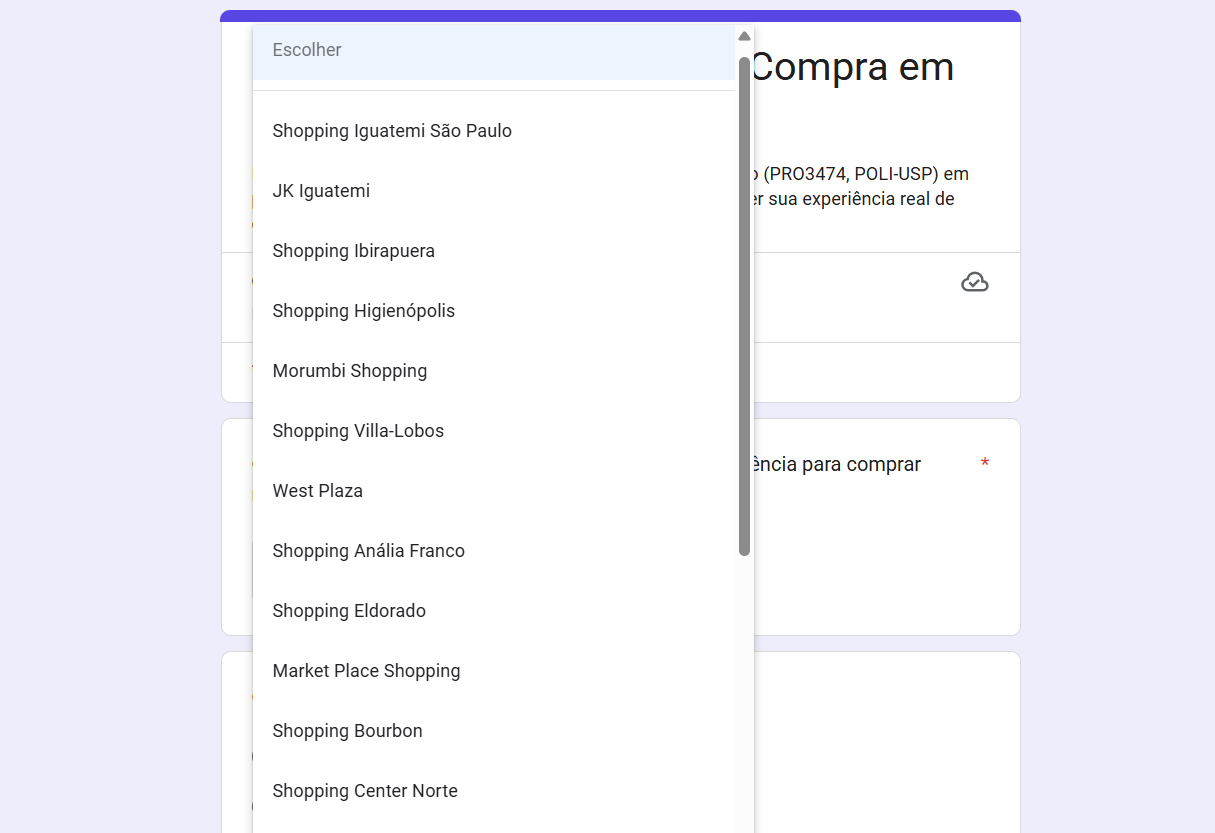
\includegraphics[width=0.5\textwidth]{imagens/pesquisa/shoppings.png}
    \label{fig:survey-qualificacao}
    \source{Autoria própria}
\end{figure}

\textbf{Aspectos investigados:} o instrumento cobre cinco dimensões, cada uma amarrada a uma das hipóteses da Seção~\ref{subsec:clientes_lacunas}: disponibilidade e facilidade de encontrar produtos; atendimento e autonomia, segmentados por momento da jornada (escolha, prova, pagamento); fila e tempo de pagamento; confiança em tecnologia e uso de canais digitais; e segurança e confiança no processo de saída da loja.

\begin{figure}[H]
    \centering
    \caption{Exemplo de bloco de afirmações em escala de concordância}
    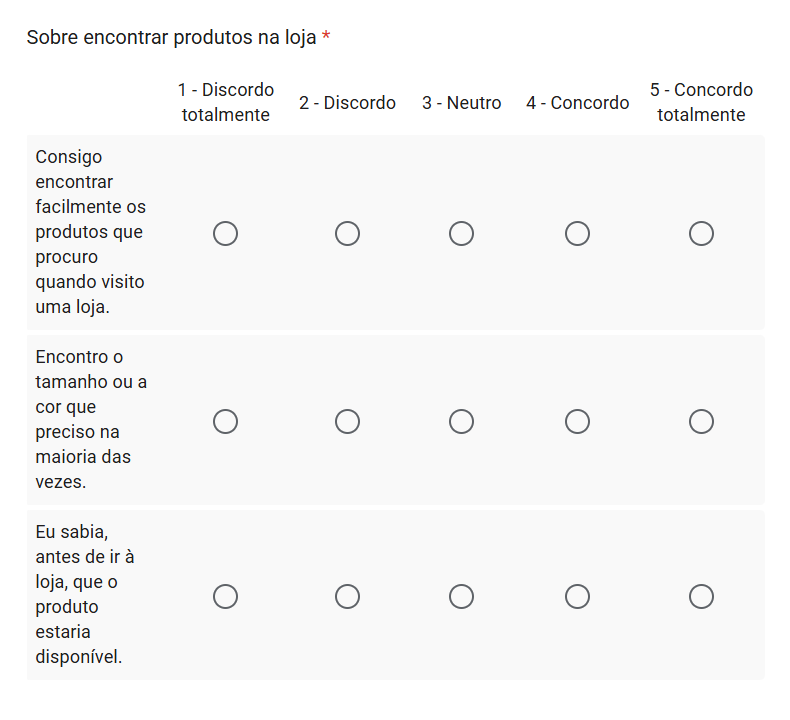
\includegraphics[width=0.5\textwidth]{imagens/pesquisa/likert.png}
    \label{fig:survey-bloco-concordancia}
    \source{Autoria própria}
\end{figure}

\begin{figure}[H]
    \centering
    \caption{Exemplo de pergunta de frequência}
    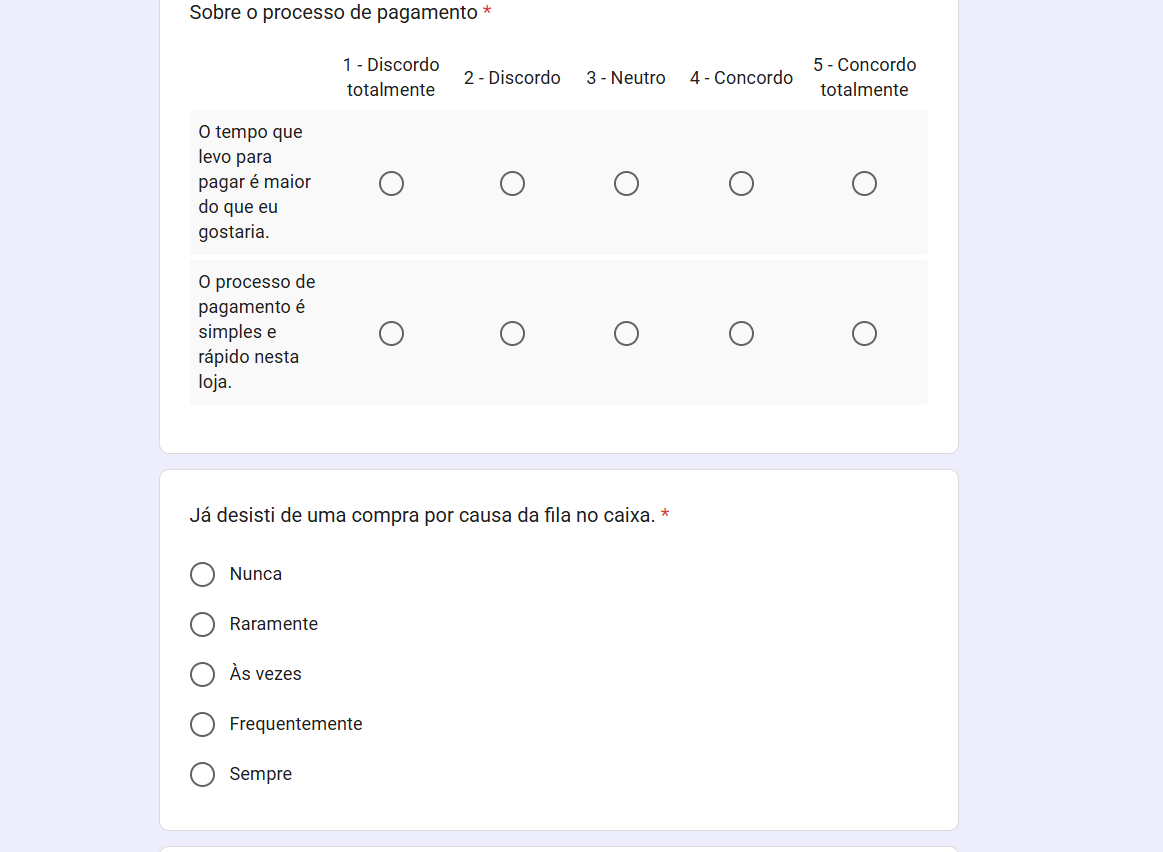
\includegraphics[width=0.5\textwidth]{imagens/pesquisa/desistencia.png}
    \label{fig:survey-pergunta-frequencia}
    \source{Autoria própria}
\end{figure}

O survey mede quantas pessoas relatam cada fricção e com que intensidade. As entrevistas explicam por que essas fricções ocorrem e em que contexto. Nenhuma das duas frentes isolada responde às duas perguntas ao mesmo tempo, e por isso a equipe as conduz em paralelo.

A classificação por unidade frequentada assume que cada loja tem um perfil predominante único. Isso falha em dois casos: um respondente frequenta mais de uma unidade com perfis diferentes, ou uma unidade tem público misto, como uma loja de rua em bairro de alta renda. O instrumento também depende de autorrelato, sujeito aos mesmos vieses de qualquer survey de autopercepção: um respondente pode subestimar comportamentos que julga socialmente indesejáveis, como depender do vendedor para decidir uma compra.

\newpage% Fragmento para incorporação ao relatório principal do projeto PRO3474.
% Pacotes pressupostos no preâmbulo do documento que incorporar este arquivo:
%   inputenc (utf8), fontenc (T1), graphicx, longtable, booktabs, array, geometry (margens compatíveis com tabelas largas).
% Figuras referenciadas em figures/ (caminho relativo a este arquivo).

\section{Análise dos clientes}

\subsection{Fontes e abordagem metodológica}

Esta análise teve como objetivo responder a três perguntas: quem são os clientes observados na experiência de compra em loja física da Riachuelo, como esses clientes podem ser agrupados a partir de comportamentos e contextos relevantes para a jornada de compra, e o que esses clientes procuram, valorizam ou enfrentam ao longo dessa jornada. A tradução desses achados em necessidades, desejos e demandas preliminares, apresentada na Seção~\ref{sec:ndd}, foi tratada como etapa posterior, e não como ponto de partida da leitura dos dados.

Foram utilizadas duas fontes primárias, complementadas por dois documentos de apoio. A primeira fonte foi um survey estruturado, intitulado \emph{Pesquisa de Experiência de Compra em Loja}, aplicado junto a consumidores e exportado em 142 respostas válidas. O instrumento teve seis páginas e 25 campos, combinando itens de escala Likert de 1 a 5 com itens de frequência (de \emph{Nunca} a \emph{Sempre}), organizados em cinco blocos temáticos: disponibilidade e facilidade de encontrar produtos; atendimento e autonomia; filas, pagamento e tempo na loja; confiança em tecnologia e canais digitais; segurança e confiança na compra. O item central para a hipótese de solução em estudo foi \emph{Confiaria em um processo de compra que não exigisse checagem manual na saída, desde que o pagamento já estivesse confirmado}. Um problema no registro do formulário fez com que os 142 carimbos de data e hora do arquivo exportado aparecessem concentrados num intervalo de poucos minutos, embora a coleta tenha ocorrido ao longo de uma semana. Essa falha não compromete o conteúdo das respostas e não motivou a exclusão de nenhum registro: todas as 142 respostas foram usadas na análise.

A segunda fonte foi um conjunto de onze entrevistas individuais semiestruturadas, conduzidas com um roteiro dividido em blocos temáticos: abertura e contexto, reconstrução de uma jornada de compra recente, busca e disponibilidade de produto, autonomia e atendimento do vendedor, fila e pagamento, confiança e segurança, necessidades não previstas, e, apenas ao final, exploração da hipótese de solução em estudo. O roteiro foi desenhado para que o entrevistado descrevesse experiências concretas em vez de opiniões abstratas, e para que a etiqueta de segurança inteligente só fosse mencionada depois de o entrevistado relatar livremente sua jornada de compra, suas fontes de fricção e suas preferências de atendimento. Essa ordem foi respeitada na leitura dos resultados: os achados sobre caracterização e agrupamento de clientes, apresentados nas Seções~\ref{sec:caracterizacao} e \ref{sec:clusters}, não partem da solução em estudo.

Como documentos de apoio, foi consultado o roteiro de entrevista na íntegra, para confirmar a intenção de cada bloco de perguntas, e uma nota anterior sobre o desenho do survey, que descreve os cinco perfis comportamentais usados para orientar a construção do instrumento e a composição da amostra de entrevistados: autônomo digital, pragmático equilibrado, dependente de atendimento, cético tradicional e frustrado com disponibilidade. Esses cinco perfis foram tratados nesta análise como hipóteses de partida, não como resultado. Ao longo do texto, a análise mostra em que medida esses perfis se confirmam nos dados, onde se fundem, e onde um comportamento relatado não se encaixa bem em nenhum deles.

A abordagem analítica partiu dos dados brutos do survey, sem carregar os rótulos de perfil originais em nenhuma etapa de agrupamento. As perguntas foram recodificadas para escalas numéricas de 0 a 100 e combinadas em dimensões comportamentais (detalhadas na Seção~\ref{sec:quantitativa}). Sobre essas dimensões foram testados agrupamentos por \emph{k-means} e por clusterização hierárquica (Ward), comparando diferentes números de grupos pelo coeficiente de silhueta. As onze entrevistas foram lidas na íntegra, tema a tema, e as falas mais reveladoras foram organizadas por padrão de comportamento. Os rótulos de perfil originais só voltam a aparecer na Seção~\ref{sec:integracao}, para comparar o resultado emergente com o ponto de partida do projeto.

Uma limitação transversal a toda a análise deve ser registrada desde já. A amostra de 142 respostas de survey e 11 entrevistas é pequena, e os materiais disponíveis não documentam como os respondentes e entrevistados foram recrutados ou selecionados. Isso impede avaliar se a amostra é razoavelmente aleatória, concentrada por conveniência, ou enviesada por algum canal específico de recrutamento. As proporções, correlações e agrupamentos discutidos neste documento devem ser lidos como padrões observados nesta amostra específica, e não como estimativas validadas para o conjunto de clientes da Riachuelo. Onde a evidência permitir apenas uma leitura qualitativa, isso é indicado explicitamente no texto.

\subsection{Caracterização dos clientes}
\label{sec:caracterizacao}

\subsubsection{Perfil sociodemográfico e de frequência de compra}

A amostra do survey concentrou-se na faixa de 25 a 34 anos (32\% dos respondentes), seguida por 35 a 44 e 45 a 54 anos (17\% cada). O gênero predominante foi feminino (53\%), seguido de masculino (42\%), com uma pequena parcela não binária ou que preferiu não informar. A frequência de compra em loja física dividiu-se entre \emph{mensalmente} (44\%) e \emph{algumas vezes ao ano} (43\%), com uma minoria comprando mais de uma vez por mês (13\%). A amostra distribuiu-se por vinte shoppings e regiões diferentes de São Paulo e Campinas, sem concentração forte em nenhum, o que limita qualquer leitura por loja específica (Figura~\ref{fig:perfil_demografico}).

\begin{figure}[htbp]
    \centering
    \textbf{Perfil demográfico}
    \caption{Perfil demográfico (faixa etária) e frequência de compra em loja física da amostra do survey (n = 142).}
    \label{fig:perfil_demografico}
\end{figure}

As onze entrevistas cobriram uma faixa etária mais ampla no relato, de jovens como Thiago e Luana a aposentados como Nivaldo e Robério, e uma variedade de papéis de compra (para si, para o cônjuge, para os filhos, para o próprio negócio) que o survey não capturou diretamente, mas que ajudou a interpretar o que estava por trás das respostas de escala.

Como será mostrado na Seção~\ref{sec:quantitativa}, a idade apresentou associação apenas moderada com o comportamento observado, e outras variáveis demográficas, como gênero e loja frequentada, explicaram uma fração ainda menor da variação entre respondentes. Por esse motivo, esta análise não reduziu a caracterização dos clientes a variáveis sociodemográficas: os comportamentos relatados a seguir mostraram maior poder explicativo.

\subsubsection{Papel da compra: para si e para terceiros}

A maioria dos episódios relatados nas entrevistas envolveu compra para o próprio entrevistado. Uma entrevista, a de Wagner, descreveu uma jornada estruturalmente distinta: comprar roupa para os três filhos, sem eles presentes. Nesse caso, a incerteza não recaiu sobre o que comprar (cor, modelo), e sim sobre uma variável que o comprador não podia verificar sozinho, o corpo de outra pessoa: \emph{"Foi bem tentando adivinhar, sinceramente. Eu tirei uma foto da etiqueta de uma calça dele em casa antes de sair, mas mesmo assim eu fico inseguro porque cada marca tem um tamanho diferente"} (Entrevista 10). O survey não tem nenhum item que identifique para quem a peça está sendo comprada, o que impede estimar, a partir dos dados quantitativos, que fração da amostra vive uma situação semelhante à de Wagner.

\subsubsection{Companhia na compra e contexto emocional}

As entrevistas revelaram uma variação relevante no papel da companhia durante a compra, distinta simplesmente de ir sozinho ou acompanhado. Para Marisa e Robério, ir acompanhado (da filha, da esposa) funcionou como um recurso de apoio à decisão: \emph{"Ela que me ajuda a escolher, porque sozinho eu me perco um pouco"} (Entrevista 3). Para Camila, a companhia de uma amiga fez parte do caráter de lazer da visita, sem relação com dependência de decisão: a compra funcionou como \emph{"um passeio"}, não como tarefa. Essa distinção é relevante porque um mesmo comportamento superficial (comprar acompanhado) correspondeu a motivações diferentes: apoio à decisão em um caso, experiência social recreativa em outro. O survey não permite separar essas duas motivações, já que não perguntou sobre companhia na compra.

\subsubsection{Autonomia como preferência variável por etapa da jornada, não como traço fixo}

Um padrão recorrente nas entrevistas foi a coexistência, na mesma pessoa, de preferência por resolver uma etapa da jornada sozinha e de dependência de ajuda em outra etapa, sem que isso fosse relatado como contradição pelo próprio entrevistado. Camila descreveu essa divisão de forma direta: \emph{"A parte de escolher e experimentar, com certeza. Gosto de fazer isso no meu ritmo, sem ninguém em cima"}, e, na mesma entrevista, sobre o que uma vendedora resolve que ela não resolveria sozinha: \emph{"Achar tamanho que sumiu da araque, isso sim eu peço ajuda"} (Entrevista 8). O mesmo padrão apareceu, com variações, em quase todas as entrevistas: a autonomia desejada concentrou-se na escolha e na experimentação, e cedeu lugar à dependência de ajuda especificamente quando o produto procurado não estava visível ou disponível na araque. Esse achado qualitativo sugere que autonomia, tal como o survey a mede (um único conjunto de itens agregados em uma dimensão, ver Seção~\ref{sec:quantitativa}), pode não corresponder a um traço estável do cliente, e sim a uma preferência que varia por etapa da jornada. Essa é uma interpretação construída a partir das entrevistas, não uma medição direta, já que o survey não testou autonomia separadamente por etapa.

\subsubsection{Busca de produto e confiança em canais digitais}

A dificuldade de localizar produtos dentro da loja apareceu com frequência distinta entre entrevistados, mas de forma quase universal em algum grau. Marisa relatou: \emph{"Demais. Principalmente pra mim mesma, que eu uso um tamanho que sempre falta. Isso é bem frequente, viu"} (Entrevista 1). Três entrevistados (Joyce, Felipe e Renata) relataram, de forma independente, ter perdido confiança na informação de estoque exibida por site ou aplicativo depois de uma experiência de divergência entre o que viram online e o que encontraram na loja: \emph{"Porque já aconteceu de eu ver uma coisa disponível no site e chegar lá e não achar, aí acabei desconfiando, sabe. Prefiro ir olhar com meus próprios olho"} (Joyce, Entrevista 2). Esse padrão qualitativo é relevante porque uma parcela da amostra parte de uma credibilidade já corroída em relação a canais digitais de disponibilidade, e não de uma expectativa neutra, o que a leitura puramente quantitativa do item correspondente do survey (Seção~\ref{sec:quantitativa}) não captura sozinha.

\subsubsection{Sensibilidade a fila e a provador}

A definição de problema vigente no projeto trata o intervalo entre decidir comprar e conseguir sair da loja como o núcleo da fricção observada. As entrevistas confirmaram esse intervalo como fonte real de fricção para parte dos entrevistados, mas também apontaram um contraponto que a formulação atual do problema não cobre: para quem valorizou atendimento, a fricção mais citada não foi a fila do caixa, e sim a fila do provador ou a espera por um vendedor disponível. Marisa descreveu o provador como algo recorrente, não excepcional: \emph{"Acho que o provador é uma coisa que pesa bastante, viu. Poucas cabine, fila grande, isso atrapalha demais, principalmente em dia de promoção"} (Entrevista 1). Esse achado qualitativo devolve à definição de problema um contraponto específico de escopo: a fricção entre decidir comprar e sair da loja pode incluir etapas anteriores ao caixa, como prova e disponibilidade de cabine, que a formulação centrada no destravamento pós-pagamento não cobre diretamente.
\subsection{Identificação dos grupos de clientes}
\label{sec:clusters}

\subsubsection{Da hipótese de cinco perfis a uma tipologia de quatro grupos}

O survey foi originalmente desenhado a partir de cinco perfis hipotéticos: consumidoras com menor autonomia e maior insegurança tecnológica, consumidores orientados à eficiência, consumidoras orientadas à experiência e conveniência, pessoas comprando para terceiros (sobretudo filhos), e um grupo residual de respondentes diversos. Esses cinco perfis orientaram o desenho do instrumento e a composição da amostra de entrevistados, e foram tratados nesta análise como hipóteses de partida a verificar, não como categorias obrigatórias de segmentação.

A verificação partiu da estrutura de correlação entre cinco dimensões comportamentais construídas a partir dos itens do survey: autonomia (preferência por resolver e pagar sozinho, com os itens de dependência de vendedor invertidos), confiança em tecnologia, pré-pesquisa digital (consulta a site ou aplicativo antes de ir à loja), sensibilidade à fila, e dor de disponibilidade (dificuldade de encontrar tamanho ou cor, desconhecimento prévio de estoque, saídas sem comprar). A Figura~\ref{fig:correlacao} mostra que quatro dessas cinco dimensões, autonomia, confiança em tecnologia, pré-pesquisa digital e sensibilidade à fila, se correlacionaram fortemente entre si (0,77 a 0,92): nesta amostra, quem se mostrou mais autônomo também confiou mais em tecnologia, pesquisou mais antes de ir à loja e se incomodou mais com fila. A dor de disponibilidade, em contraste, mostrou-se quase independente das outras quatro (correlações entre $-0,22$ e $0,15$).

\begin{figure}[htbp]
    \centering
    \textbf{Correlação}
    \caption{Correlação entre as cinco dimensões comportamentais construídas a partir do survey (n = 142).}
    \label{fig:correlacao}
\end{figure}

Esse é um dado observado, não uma interpretação: as correlações medidas nesta amostra reduzem o espaço de diferenciação real a duas dimensões, e não cinco. A explicação para a alta correlação entre as quatro primeiras dimensões permanece como hipótese em aberto: pode refletir um traço de disposição coerente, no qual pessoas com rotina mais apertada tendem a ser, ao mesmo tempo, mais adeptas de tecnologia, mais autônomas e mais impacientes com fila, ou pode refletir, ao menos em parte, um viés de resposta comum em survey de autorrelato, no qual respondentes tendem a concordar ou discordar de forma consistente ao longo de itens redigidos de forma parecida, independentemente do conteúdo específico de cada um. Os dados atuais não permitem separar as duas explicações. As entrevistas trazem ao menos um contraexemplo direto a uma fusão automática entre autonomia e confiança em tecnologia: Nivaldo descreveu-se como autônomo na escolha do produto, mas desconfiado do pagamento por celular (Entrevista 5), o que reforça que a fusão observada no survey deve ser lida como um padrão desta amostra, não como lei geral de comportamento do consumidor.

A partir dessa constatação, os agrupamentos foram construídos sobre duas dimensões não redundantes: um índice combinado de autonomia, confiança em tecnologia, pré-pesquisa digital e sensibilidade à fila, chamado nesta análise de orientação autonomia-tecnologia-eficiência, e a dor de disponibilidade, mantida separada por ser quase independente da primeira. Foram testados \emph{k-means} e clusterização hierárquica (Ward) para números de grupo entre 2 e 7, comparando o coeficiente de silhueta de cada solução. Os dois métodos convergiram para os mesmos números e tamanhos de grupo. O melhor equilíbrio entre coesão dos grupos e interpretabilidade, sem grupo residual muito pequeno, apareceu em quatro grupos (silhueta de 0,55; uma solução com cinco grupos melhorou marginalmente a silhueta ao custo de isolar um grupo de apenas nove respondentes, tratado como ruído estatístico e não como um quinto agrupamento).

Essa clusterização formal deve ser lida pelo que é: uma técnica exploratória aplicada a 142 respostas de survey, com itens de escala de variação adequada para sustentá-la, e não o critério final e definitivo dos agrupamentos de clientes da Riachuelo. A Seção~\ref{sec:integracao} cruza os quatro grupos identificados com o material qualitativo das entrevistas, e ajusta a interpretação onde a evidência qualitativa exige nuance que a clusterização quantitativa, isoladamente, não captura.

\begin{figure}[htbp]
    \centering
    \includegraphics[width=0.8\textwidth]{imagens/Poli.png}
    \caption{Distribuição dos respondentes nos dois eixos usados para a clusterização exploratória: orientação autonomia-tecnologia-eficiência e dor de disponibilidade (n = 142).}
    \label{fig:clusters_scatter}
\end{figure}

\begin{figure}[htbp]
    \centering
    \includegraphics[width=0.8\textwidth]{imagens/Poli.png}
    \caption{Tamanho dos quatro agrupamentos exploratórios identificados (n = 142).}
    \label{fig:tamanho_clusters}
\end{figure}

Os quatro grupos que emergiram não reproduziram exatamente os cinco perfis originais do survey. Três deles tiveram tamanho relativamente próximo a três dos perfis originais, o que sugere que o instrumento os capturou razoavelmente bem. O quarto perfil original, cético tradicional, não apareceu como grupo separado: seus 13 respondentes esperados parecem ter se fundido ao grupo de menor autonomia, junto com o antigo perfil dependente de atendimento (39 mais 13 igual a 52, próximo aos 55 respondentes observados nesse grupo). Esse resultado foi tratado como achado, não como erro de método, e é discutido na Seção~\ref{sec:cluster_aberto} e retomado na síntese (Seção~\ref{sec:sintese}).

As Figuras~\ref{fig:confianca_cluster} e \ref{fig:desistencia_cluster} comparam os quatro grupos nos dois itens mais decisivos da análise: a reação ao conceito de desbloqueio sem checagem manual, e a frequência com que os respondentes já desistiram de uma compra por causa de fila. Ambas mostram um padrão qualitativamente diferente entre grupos, e não apenas de intensidade diferente, o que orientou a construção das fichas de cada cluster a seguir.

\begin{figure}[htbp]
    \centering
    \includegraphics[width=0.8\textwidth]{imagens/Poli.png}
    \caption{Distribuição de respostas ao item de confiança em processo de compra sem checagem manual na saída, por agrupamento (n = 142).}
    \label{fig:confianca_cluster}
\end{figure}

\begin{figure}[htbp]
    \centering
    \includegraphics[width=0.8\textwidth]{imagens/Poli.png}
    \caption{Frequência com que os respondentes já desistiram de uma compra por causa da fila, por agrupamento (n = 142).}
    \label{fig:desistencia_cluster}
\end{figure}

\subsubsection{Cluster 1: dependentes de atendimento}

Este foi o maior dos quatro grupos, com 55 de 142 respondentes (39\%). Apresentou a menor pontuação de orientação autonomia-tecnologia-eficiência dos quatro grupos (média de 30,1 em uma escala de 0 a 100) e a maior importância atribuída ao vendedor na hora de experimentar a peça, com concordância unânime nesse item. O comportamento observado combinou baixa sensibilidade a fila (76\% raramente e 22\% nunca desistiram de comprar por causa de fila) com baixa confiança em pagar por celular (73\% discordam ou discordam totalmente) e baixo conhecimento prévio de disponibilidade do produto antes de ir à loja. O contexto típico de compra, segundo as entrevistas associadas a este padrão, envolveu a presença desejada de um vendedor tanto para confirmar a escolha quanto para localizar tamanhos fora da araque. A fricção mais frequente relatada não foi a fila do caixa, e sim a ausência ou demora de um vendedor no momento de escolha e prova. A reação ao conceito de desbloqueio sem checagem manual foi de rejeição quase unânime (96\% discordam ou discordam totalmente, com uma pequena fração neutra e nenhuma concordância).

Este grupo foi, ao mesmo tempo, o mais homogêneo nas duas dimensões usadas para a clusterização e o mais heterogêneo em termos de motivação qualitativa. As entrevistas sugerem que ele reúne ao menos duas motivações distintas por trás de um comportamento de escala semelhante: pessoas que valorizam a companhia e a opinião de um vendedor como parte positiva da experiência, como Marisa, para quem ir à loja funciona como \emph{"um respiro"}, e pessoas que relatam desconfiança de tecnologia e de mudança em si, como Robério, para quem a hipótese de solução \emph{"deixa bem inseguro"} (Entrevista 3). O survey não distingue essas duas motivações; as entrevistas sim. Marisa, sobre o que a faria confiar em um processo sem checagem: \emph{"Confiaria mais se soubesse que tem alguém pra me ajudar caso desse algum problema. Sozinha eu fico insegura"} (Entrevista 1).

\subsubsection{Cluster 2: autônomos digitais}

Este grupo reuniu 30 de 142 respondentes (21\%) e apresentou a maior pontuação de orientação autonomia-tecnologia-eficiência dos quatro grupos (média de 80,8) e a menor importância atribuída ao vendedor na prova (97\% discordam ou discordam totalmente desse item, com 3\% neutro). Foi, simultaneamente, o grupo mais autônomo e o mais incomodado com fila: a totalidade já desistiu de comprar por causa de fila em algum grau, e 17\% relataram isso como algo frequente, a maior taxa entre os quatro grupos. Concentrou a faixa etária mais jovem da amostra (76\% com menos de 35 anos). O contexto típico envolveu uma rotina de tempo apertado, uso corrente de autoatendimento, pagamento por aproximação e pix fora da loja, e busca por velocidade e controle sobre o próprio processo de compra. A fricção mais frequente relatada foi especificamente o tempo perdido em fila, não a dificuldade de achar produto nem a falta de ajuda. A reação ao conceito de desbloqueio sem checagem manual foi a única com aceitação majoritária entre os quatro grupos (100\% concordam ou concordam totalmente, sem nenhuma resposta neutra ou negativa).

Este foi o grupo com maior consistência entre discurso e comportamento relatado: quem afirmou preferir autonomia também foi quem, nas entrevistas correspondentes, efetivamente resolveu a compra sozinho. Thiago, sobre a hipótese de solução: \emph{"Achei sensacional, sinceramente. Resolve exatamente o que eu mais odeio, que é fila"} (Entrevista 6). Felipe, no mesmo sentido, propôs por iniciativa própria estender a ideia para \emph{"avisar estoque em tempo real"} (Entrevista 4), o que indica que, para este grupo, a hipótese de solução foi entendida como potencial ponto de partida para uma integração digital mais ampla, e não apenas como um mecanismo de destravamento.

\subsubsection{Cluster 3: frustrados com disponibilidade}

Este foi o menor dos quatro grupos, com 13 de 142 respondentes (9\%), e o único cujo tamanho coincidiu quase exatamente com o do perfil equivalente na hipótese original de cinco perfis (também 13). Apresentou a maior dor de disponibilidade dos quatro grupos, por larga margem (média de 78,8 em 100, contra 46,5 a 54,5 nos demais grupos), com orientação autonomia-tecnologia-eficiência em nível intermediário-alto (60,6), nem o mais dependente nem o mais autônomo. A totalidade dos respondentes deste grupo relatou sair da loja frequentemente sem comprar por não encontrar o que procurava, e a totalidade discordou de encontrar o tamanho ou a cor que precisava. Foi também o grupo com maior concordância de que saber, pelo aplicativo, se um produto está disponível na loja mudaria sua decisão de se deslocar até ela. A fricção mais frequente relatada foi, de forma consistente, não encontrar tamanho, cor ou modelo, e não fila ou falta de vendedor. A reação ao conceito de desbloqueio sem checagem manual foi de neutralidade praticamente unânime, um padrão distinto dos outros três grupos, nenhum dos quais concentrou-se de forma tão uniforme em um único ponto da escala.

Essa neutralidade unânime é, em si, um dado que exige cautela interpretativa: pode refletir indiferença genuína a um conceito que não tem relação clara com a dor relatada por este grupo, ou pode refletir uma avaliação de fato indiferente. As entrevistas favorecem a primeira leitura. Wagner, comprando para os filhos sem eles presentes, associou-se a este padrão de resposta: \emph{"Achei ok, mas sinceramente não é isso que resolveria meu maior problema, que é acertar o tamanho"}, e, quando perguntado o que a hipótese de solução resolve: \emph{"Resolve uma coisa que nem era meu problema principal. Meu problema é tamanho, isso aqui resolve fila e pagamento"} (Entrevista 10).

\subsubsection{Cluster 4: pragmáticos equilibrados}

Este grupo reuniu 44 de 142 respondentes (31\%), o segundo maior dos quatro, e ocupou posição intermediária em ambas as dimensões usadas para a clusterização: nem alta nem baixa orientação autonomia-tecnologia-eficiência (53,8) e nem alta nem baixa dor de disponibilidade (49,7). O comportamento observado combinou baixa sensibilidade a fila (82\% raramente, 16\% às vezes e 2\% frequentemente desistiram por fila) com posição majoritariamente neutra em praticamente todos os itens de atitude do survey, sem discordância ou concordância forte em nenhum. A reação ao conceito de desbloqueio sem checagem manual foi majoritariamente neutra (91\%), com uma pequena inclinação à concordância (9\%, entre concordo e concordo totalmente) e nenhuma discordância registrada, uma leve tendência à aceitação, não à rejeição.

Por ser o grupo residual das duas dimensões usadas para clusterizar, este é provavelmente o mais heterogêneo internamente em termos de motivação real, e a etiqueta pragmático equilibrado descreve a posição estatística do grupo, não necessariamente uma identidade comportamental compartilhada por todos os 44 respondentes. Vale tratá-lo, nesta etapa, como o que resta depois de isolar os três padrões mais nítidos, não como um perfil positivo e coeso por si. Camila, sobre a hipótese de solução, ilustrou bem essa posição intermediária: \emph{"Achei legal a ideia, principalmente pra quando eu já sei o que quero e não preciso ficar na fila. Mas confesso que não é meu maior problema hoje"} (Entrevista 8), nem rejeição nem entusiasmo.

\subsubsection{Uma pergunta em aberto sobre o quinto perfil original}
\label{sec:cluster_aberto}

A base original foi desenhada com cinco perfis, mas a clusterização convergiu para quatro grupos nítidos. O perfil ausente, cético tradicional, parece ter se fundido ao grupo de menor autonomia (Cluster 1). Duas hipóteses concorrentes explicam essa fusão, e os dados atuais não permitem decidir entre elas. A primeira é que dependência de atendimento e ceticismo tecnológico sejam, de fato, a mesma coisa nesta população: quem depende de vendedor também desconfia de tecnologia, sem que isso represente duas motivações distintas. A segunda é que sejam motivações diferentes, uma de preferência social positiva por interação humana e outra de aversão a risco e mudança, que o instrumento de survey não tem itens específicos para separar, mas que as entrevistas sugerem existirem lado a lado dentro do mesmo cluster, como a diferença entre Marisa, para quem a loja é companhia e cuidado pessoal, e Robério, para quem qualquer novidade tecnológica gera insegurança. Essa questão é retomada na síntese final (Seção~\ref{sec:sintese}).

\subsection{Análise dos resultados da pesquisa quantitativa}
\label{sec:quantitativa}

\subsubsection{O item decisivo: confiança em processo sem checagem manual}

A distribuição de respostas ao item central para a hipótese de solução concentrou-se em discordância e neutralidade: 39\% neutros, 31\% discordam e 6\% discordam totalmente, uma maioria de 76\% que não endossou a ideia. Apenas 24\% concordaram ou concordaram totalmente (Figura~\ref{fig:confianca_geral}). A distribuição não foi bimodal, isto é, não formou dois grupos opostos e nítidos: foi assimétrica, puxada para o lado cético, com uma cauda de concordância bem menor.

\begin{figure}[htbp]
    \centering
    \includegraphics[width=0.8\textwidth]{imagens/Poli.png}
    \caption{Distribuição de respostas ao item de confiança em processo de compra sem checagem manual na saída, desde que o pagamento já esteja confirmado (n = 142).}
    \label{fig:confianca_geral}
\end{figure}

Isso sugere que, nesta amostra, o conceito de dispensar checagem manual não partiu de uma aceitação ampla: encontrou um núcleo relativamente pequeno de interesse claro, os 24\% que concordaram, e uma massa grande que nem rejeitou nem abraçou a ideia. Como mostrado na seção anterior, essa neutralidade não se distribuiu igualmente entre os quatro agrupamentos identificados, e concentrou-se em grupos específicos por motivos qualitativamente diferentes entre si, um caso em que a média geral da amostra esconde mais do que revela.

Neutralidade em um item de escala admite mais de uma leitura: pode indicar indiferença genuína, mas também pode indicar que a pergunta não fez sentido para quem respondeu, por exemplo alguém cuja dor não tem relação com checagem de saída, ou insegurança em avaliar um conceito abstrato sem uma experiência concreta para ancorar a resposta. As entrevistas ajudaram a distinguir essas leituras, e sugerem que, para vários entrevistados, a neutralidade do survey provavelmente escondeu \emph{"isso não resolve o meu problema"}, e não \emph{"não tenho opinião"}.

\subsubsection{Sensibilidade à fila: diferença por agrupamento, não por frequência de compra}

A frequência de compra declarada (algumas vezes ao ano, mensalmente, mais de uma vez por mês) não se associou de forma clara com dor de disponibilidade nem com a orientação autonomia-tecnologia-eficiência: as médias entre grupos de frequência de compra variaram menos de 8 pontos em 100, sem gradiente consistente. Comprar mais, nesta amostra, não tornou a pessoa mais nem menos autônoma, nem mais nem menos incomodada com falta de produto. Quem realmente diferiu foi o agrupamento comportamental: a fração de respondentes que já desistiu de uma compra frequentemente por causa de fila variou de 0\% a 17\% conforme o grupo, e a fração que nunca desistiu variou de 0\% a 22\%.

Essa constatação sugere que a relação entre o cliente e a fila não foi função de quanto ele compra, mas de um padrão comportamental mais amplo, o mesmo eixo de orientação autonomia-tecnologia-eficiência discutido na Seção~\ref{sec:clusters}. Essa leitura contraria a suposição de que a fila representa uma fricção universal e uniforme entre os clientes: os dados sugerem algo mais específico, fila incomodou intensamente, mas principalmente um segmento identificável da amostra, não a amostra como um todo. Vale registrar que frequência de compra é uma medida autodeclarada que não distingue ida à loja de compra efetiva: alguém que visita a loja com frequência para navegar, como o comportamento relatado por Luana, pode responder mensalmente mesmo comprando raramente.

\subsubsection{Disponibilidade de tamanho e cor: um problema concentrado, não disperso}

Olhando a amostra inteira, a maioria das respostas ao item sobre encontrar o tamanho ou a cor desejada se concentrou em torno de neutro, o que poderia sugerir um problema brando e disperso. Ao segmentar por agrupamento comportamental, no entanto, emergiu um grupo pequeno (13 de 142, 9\% da amostra) no qual a totalidade dos respondentes discordou ou discordou totalmente desse item, e a totalidade relatou sair da loja frequentemente sem comprar por não encontrar o que procurava, o oposto do padrão do restante da amostra. A leitura de que disponibilidade não é um problema generalizado mudou quando o dado foi desagregado: o problema existiu, mas concentrado com intensidade alta em um subgrupo específico, e quase ausente no resto da amostra, um padrão que a média geral escondeu e que a segmentação revelou. Com apenas 13 respondentes, esse subgrupo é pequeno demais para generalizações de proporção populacional, mesmo dentro dos limites já postos pelo tamanho e pela representatividade incerta da amostra. Seu valor aqui é qualitativo: mostrar que o padrão existiu e foi internamente consistente, não estimar que fração real de clientes da Riachuelo ele representa.

\subsubsection{Orientação autonomia-tecnologia-eficiência por faixa etária}

Houve uma tendência de queda na orientação autonomia-tecnologia-eficiência conforme a idade aumentou, de uma média de 62 (em escala de 0 a 100) entre 18 e 24 anos até valores entre 40 e 45 a partir dos 45 anos, mas a diferença entre faixas adjacentes foi pequena diante da dispersão dentro de cada faixa (Figura~\ref{fig:idade}). Existe, portanto, uma associação, mas fraca e gradual, e não um corte nítido entre jovem autônomo e idoso dependente. A dispersão dentro de cada faixa etária foi grande o bastante para que um respondente de 60 anos pontuasse mais alto em autonomia e tecnologia do que um de 25, e as entrevistas confirmaram isso com casos concretos: Nivaldo, aposentado, relatou testar autoatendimento sem problema, enquanto Débora, mais jovem, relatou depender fortemente de uma vendedora específica. Usar idade como preditor único de orientação a autonomia, a partir deste gráfico isoladamente, forçaria uma generalização que os próprios dados não sustentam: a idade parece contribuir para essa orientação, mas não a determina.

\begin{figure}[htbp]
    \centering
    \includegraphics[width=0.8\textwidth]{imagens/Poli.png}
    \caption{Orientação autonomia-tecnologia-eficiência por faixa etária (n = 142).}
    \label{fig:idade}
\end{figure}

\subsubsection{Qualidade e limitações da base quantitativa}

Alguns itens do survey apresentaram pouca variação e, por isso, pouca utilidade para diferenciar respondentes: consigo encontrar facilmente os produtos que procuro (82\% neutro), encontro o tamanho ou a cor que preciso (87\% neutro), um vendedor te aborda com que frequência (92\% às vezes), já me senti desconfortável com verificação na saída (99\% nunca ou raramente). Esses itens foram mantidos na base, mas pesaram pouco nas dimensões construídas. Os itens com melhor variação, e por isso mais informativos, foram os cinco itens do bloco de autonomia e atendimento, os três itens de confiança em tecnologia, e o item decisivo de aceitação do desbloqueio sem checagem manual, sobre os quais a análise de clusters se apoiou.
\subsection{Análise das entrevistas qualitativas}
\label{sec:qualitativa}

Esta seção aprofunda padrões que o survey, por sua natureza fechada, não capturou sozinho. A leitura das onze entrevistas foi conduzida tema a tema, e não entrevista a entrevista, para permitir comparação direta entre relatos.

\subsubsection{Contradição entre autonomia na prova e dependência na busca}

Como já indicado na Seção~\ref{sec:caracterizacao}, vários entrevistados relataram, na mesma conversa, preferir resolver sozinhos uma etapa da jornada e depender fortemente de ajuda em outra, sem tratar isso como contradição. Esse achado qualitativo é relevante porque sugere que autonomia não é uma preferência de traço único, como o survey a trata ao reduzi-la a um único conjunto de itens agregados, e sim uma preferência que varia conforme a etapa da jornada, especificamente cedendo lugar à dependência de ajuda quando o produto procurado não está visível ou disponível.

\subsubsection{Perder contato com quem ajuda pesa mais que falha técnica, para quem já depende de ajuda}

Uma das perguntas finais do roteiro pediu que o entrevistado escolhesse entre dois receios: a tecnologia falhar, ou perder contato com alguém que ajuda quando precisa. A resposta divergiu de forma consistente com o padrão comportamental do entrevistado, e não pareceu uma preocupação universal. Marisa respondeu: \emph{"Perder o contato com quem ajuda, com certeza. Pra mim isso é mais importante que a tecnologia funcionar direitinho"} (Entrevista 1). Wagner respondeu de forma equivalente: \emph{"Perder contato com quem ajuda, porque é dessa ajuda que eu mais preciso, mais do que da tecnologia em si"} (Entrevista 10). Thiago, no extremo oposto de autonomia, sequer tratou isso como dilema, e não mencionou a possibilidade de precisar de ajuda ao reagir à hipótese de solução. Isso indica que a resistência à ideia de destravamento remoto, onde apareceu, não foi necessariamente resistência à tecnologia em si (falha técnica), e sim resistência a perder um vínculo de suporte que a pessoa já usa e valoriza hoje.

\subsubsection{Risco reputacional: o medo de ser mal interpretado}

Uma nuance apareceu de forma explícita em apenas uma entrevista, mas merece registro por descrever um tipo de preocupação distinto de falha técnica. Marisa relatou: \emph{"Fico pensando, e se der algum erro e a etiqueta não destravar, ou pior, destravar errado e eu ser acusada de estar levando sem pagar? Isso me preocupa mais do que me anima, sinceramente"} (Entrevista 1). Essa fala descreveu um risco reputacional e social, o de ser vista como estivesse furtando, distinto do risco técnico de o sistema não funcionar e do risco financeiro de ser cobrada de forma incorreta, mencionado por Robério em relação a autoatendimento de supermercado (Entrevista 3). Os três tipos de risco parecem coexistir nas entrevistas, sem que os dados atuais indiquem qual pesa mais para o conjunto da amostra: o survey não tem item específico para risco reputacional, uma lacuna a registrar como hipótese em aberto, não uma conclusão a forçar.

\subsubsection{O vendedor como pessoa nomeada, não como função genérica}

Em duas entrevistas, a relação com o vendedor não foi descrita como atendimento genérico, e sim como relação pessoal com alguém específico, ao ponto de a entrevistada nomeá-la. Débora, sobre a vendedora que a atende há dois anos: \emph{"Ela filtra as opção pra mim, eu tenho pouco tempo, então isso é essencial, evita eu perder tempo vendo coisa que não combina"}, e, sobre a hipótese de solução: \emph{"Fico com um pé atrás, viu, porque isso parece tirar justamente a parte que eu mais valorizo, que é a pessoa envolvida no processo"} (Entrevista 9). Renata descreveu uma relação equivalente com sua consultora fixa, e distinguiu explicitamente entre usar uma solução mais autônoma \emph{"pra uma reposição rápida"} (aceitável) e usar em uma compra que envolve escolha completa com a consultora (não substituível, Entrevista 7). Esse padrão, vendedor como relação individual não intercambiável, é qualitativamente diferente da dependência de atendimento genérica medida pelo survey, e ajuda a explicar por que o Cluster 1 (dependentes de atendimento) reuniu tanto motivação de conforto e insegurança, como em Marisa e Robério, quanto motivação de relação de confiança construída ao longo do tempo, como em Débora e Renata.

\subsubsection{Uma entrevistada fora da curva}

Luana, estudante de moda que entra em lojas quase toda semana mas compra a cada dois ou três meses, não se encaixou com conforto em nenhum dos quatro agrupamentos descritos na Seção~\ref{sec:clusters}. Apresentou alta autonomia, quase nunca buscando vendedor, mas não por eficiência ou pressa, e sim por preferência de observar sozinha, sem meta de compra definida. Sua reação à hipótese de solução foi reveladora dessa diferença: \emph{"Não resolve nada do que eu mencionei, resolve um problema que eu acho que é mais de outro tipo de cliente, não o meu caso"} (Entrevista 11). Luana foi também a única entrevistada a levantar uma preocupação de dados e privacidade em relação à etiqueta inteligente, \emph{"penso em quanto dado estão coletando sobre isso"}, tema que nenhum outro entrevistado mencionou e que o survey não investigou diretamente. Esse é um sinal isolado, não um padrão, mas um sinal que a análise não deveria descartar apenas por aparecer uma única vez.

\subsection{Integração entre evidências quantitativas e qualitativas}
\label{sec:integracao}

Os quatro agrupamentos identificados na Seção~\ref{sec:clusters} encontraram correspondência razoável nas entrevistas, mas a correspondência não foi perfeita, e as diferenças foram informativas.

O Cluster 1 (dependentes de atendimento) correspondeu a Marisa, Robério, Débora e, parcialmente, Renata. O survey mostrou rejeição quase unânime ao conceito de desbloqueio sem checagem neste grupo; as entrevistas explicaram o porquê, com nuance que o survey não capturou: Robério rejeitou por desconfiança de tecnologia e mudança, Marisa rejeitou por medo de ficar sem suporte caso algo desse errado, e Débora rejeitou porque a proposta reduziria o papel da pessoa que ela mais valoriza no processo. Três motivos distintos produziram a mesma resposta de escala, exatamente o tipo de heterogeneidade já sinalizado na Seção~\ref{sec:cluster_aberto}.

O Cluster 2 (autônomos digitais) correspondeu a Thiago e Felipe de forma mais direta: o survey mostrou aceitação total e a maior taxa de desistência por fila entre os quatro grupos; as entrevistas mostraram os mesmos dois entrevistados relatando episódios concretos de desistência por fila (Black Friday, hora de almoço) e reação entusiasmada ao conceito, sem ressalva relevante. Foi o cluster onde discurso, comportamento relatado e reação ao conceito mais convergiram.

O Cluster 3 (frustrados com disponibilidade) correspondeu a Wagner e, parcialmente, a Nivaldo. O survey isolou um grupo pequeno e nitidamente definido por dificuldade de achar tamanho ou cor; Wagner confirmou esse padrão de forma direta, com uma causa específica, comprar para os filhos sem eles presentes, que o survey não captura como variável mas que produziu o mesmo padrão de resposta. Nivaldo se aproximou parcialmente deste grupo, já que sua queixa central também foi disponibilidade (tamanhos maiores), embora tivesse sido originalmente associado ao perfil de eficiência, não ao de disponibilidade. Esse é um exemplo direto de um perfil original sendo contrariado pelo comportamento relatado.

O Cluster 4 (pragmáticos equilibrados) correspondeu a Camila e, parcialmente, a Joyce. O grupo residual do survey, com posição intermediária em tudo, encontrou em Camila uma ilustração razoável: reação morna ao conceito, sem fricção aguda relatada, fila tolerada fora de datas especiais. Joyce se encaixou apenas parcialmente, sendo mais eficiente e apressada do que a média deste cluster sugeriria, o que é coerente com o próprio survey mostrar este grupo como o mais heterogêneo internamente.

Duas coisas apareceram nas entrevistas sem equivalente claro na estrutura de quatro grupos do survey, e vale destacá-las em vez de forçar seu encaixe: a relação nomeada com um vendedor específico (Débora, Renata), qualitativamente distinta de concordar com o item sobre importância do vendedor, e o perfil de baixa frequência e alta autonomia por desinteresse, não por eficiência (Luana), que não se explicou bem por nenhuma combinação das duas dimensões usadas na clusterização. Ambas ficam registradas como limite do que a segmentação quantitativa, isoladamente, conseguiu capturar.
\subsection{Necessidades, desejos e demandas dos clientes}
\label{sec:ndd}

\subsubsection{Nota metodológica}

Esta seção traduziu os achados das Seções~\ref{sec:caracterizacao} a \ref{sec:integracao} em formulações de necessidade, desejo e demanda, seguindo a distinção clássica de Kotler entre necessidade (estado em que se percebe alguma privação), desejo (necessidade humana moldada pela cultura e por características individuais, que pode ser representada por diferentes bens capazes de satisfazê-la) e demanda (desejo associado a um contexto concreto de comportamento, disposição de compra ou expectativa explicitamente manifestada). Operacionalmente, esta análise tratou como necessidade uma condição ou resultado que o cliente valorizou como relevante para realizar a jornada de compra de forma adequada; como desejo uma preferência ou expectativa cuja ausência não impede a compra nem gera uma falha fundamental na experiência; e como demanda uma necessidade ou desejo associado a um comportamento recorrente, um contexto concreto de compra ou uma expectativa explicitamente manifestada pelo entrevistado. A classificação evitou um erro comum: tratar como demanda um item apenas porque a fala que o sustenta foi emocionalmente intensa. Intensidade de fala não equivale a demanda; o critério usado foi a presença de um comportamento concreto e recorrente por trás da fala, não o tom em que ela foi dita.

Cada item a seguir foi formulado na perspectiva do resultado desejado pelo cliente, independentemente da hipótese de solução em estudo, e não foi tratado como requisito de produto. Itens semelhantes, mas associados a contextos, comportamentos ou benefícios distintos, foram mantidos separados, sem consolidação prematura. A matriz da Seção~\ref{sec:matriz} reúne todos os itens com sua rastreabilidade às evidências.

\subsubsection{Necessidades identificadas}

\textbf{N01. Ter apoio humano disponível para confirmar decisões de compra e auxiliar na experimentação da peça.} Associada principalmente ao Cluster 1 (dependentes de atendimento, 39\% da amostra) e, com menor intensidade, ao Cluster 4. Evidência quantitativa: concordância unânime com a importância do vendedor na prova e 96\% de rejeição ao item de confiança em processo sem checagem, ambos no Cluster 1. Evidência qualitativa: Marisa (Entrevista 1) descreveu a loja como um momento em que confia menos no próprio julgamento sem uma opinião externa; Robério (Entrevista 3) relatou que, sem vendedor disponível, provavelmente sairia sem comprar. Contexto: momento de escolha e experimentação da peça. Interpretação: para este grupo, a presença de um vendedor não funciona apenas como recurso instrumental para achar tamanho, mas como parte do valor da experiência ou da confiança na própria decisão. Contradição: dentro do mesmo cluster coexistem motivações distintas, uma de sociabilidade positiva e outra de aversão a risco e mudança (Seção~\ref{sec:cluster_aberto}), o que a formulação única desta necessidade não distingue. Limitação: o survey mede importância do vendedor com um único item, insuficiente para separar essas duas motivações.

\textbf{N02. Ter garantia de que existe apoio disponível caso algo dê errado em um processo de compra menos assistido.} Associada ao Cluster 1. Evidência quantitativa: 96\% de rejeição ao item de confiança em processo sem checagem manual no Cluster 1. Evidência qualitativa: quando confrontados com a escolha entre tecnologia falhar e perder contato com quem ajuda, Marisa, Robério e Wagner priorizaram o segundo receio (Entrevistas 1, 3 e 10); Marisa declarou diretamente que perder esse contato \emph{"é mais importante que a tecnologia funcionar direitinho"}. Contexto: qualquer processo de compra com menor mediação humana. Interpretação: a resistência a processos menos assistidos, onde presente, parece relacionar-se menos ao funcionamento técnico da solução e mais ao risco de ficar sem a quem recorrer. Contradição: Thiago (Entrevista 6), do Cluster 2, não tratou essa escolha como dilema relevante, o que reforça que esta necessidade não é transversal à amostra. Limitação: a pergunta que originou essa evidência foi feita apenas na etapa final da entrevista, depois de o conceito de solução já ter sido apresentado, o que pode ter induzido a resposta.

\textbf{N03. Encontrar o tamanho, a cor ou o modelo procurado dentro de um esforço razoável.} Associada principalmente ao Cluster 3 (frustrados com disponibilidade, 9\% da amostra), presente em menor grau nos demais clusters. Evidência quantitativa: no Cluster 3, totalidade dos respondentes discorda de encontrar o tamanho ou a cor que precisa, e totalidade relata sair da loja frequentemente sem comprar por esse motivo. Evidência qualitativa: Marisa (Entrevista 1) relatou que essa dificuldade é \emph{"bem frequente"} para o próprio tamanho; Nivaldo (Entrevista 5) atribuiu a mesma dificuldade à própria estatura acima da média. Contexto: busca de produto dentro da loja, antes de qualquer decisão de compra. Interpretação: esta necessidade é intensa e concentrada em um subgrupo pequeno e nitidamente definido, e quase ausente no restante da amostra, um padrão que a média geral do survey esconde. Contradição: nenhuma identificada além da concentração já descrita. Limitação: com apenas 13 respondentes no Cluster 3, o valor desta evidência é qualitativo, não uma estimativa de proporção populacional.

\textbf{N04. Obter ajuda para localizar uma peça que não está exposta ou disponível na araca de venda.} Transversal, mais forte nos Clusters 1 e 3. Evidência quantitativa: item de importância do vendedor concentrado em concordância no Cluster 1; correlação entre dor de disponibilidade e busca de ajuda relatada nas entrevistas. Evidência qualitativa: Marisa (Entrevista 1), Camila (Entrevista 8) e Nivaldo (Entrevista 5) relataram recorrer a um vendedor especificamente para verificar estoque quando o item não estava na araca. Contexto: ocorre depois de uma busca inicial sem sucesso pelo próprio cliente. Interpretação: esta necessidade é distinta de N01, já que não envolve apoio à decisão, e sim acesso a um estoque que o cliente sozinho não alcança. Contradição: nenhuma identificada. Limitação: o survey não distingue estoque em araca de estoque em depósito, o que limita a precisão desta leitura.

\textbf{N05. Confiar que a informação de estoque exibida em canais digitais corresponde à realidade da loja física.} Transversal, evidência concentrada nas entrevistas. Evidência quantitativa: não medida diretamente pelo survey, uma lacuna do instrumento. Evidência qualitativa: Joyce (Entrevista 2), Felipe (Entrevista 4) e Renata (Entrevista 7) relataram, de forma independente, ter perdido confiança na informação de estoque de site ou aplicativo após uma divergência entre o que viram online e o que encontraram na loja. Contexto: pesquisa prévia à visita à loja. Interpretação: uma parte da amostra parte de uma credibilidade já corroída em relação a canais digitais de disponibilidade, e não de uma expectativa neutra, o que qualquer solução futura que dependa de exibir disponibilidade pelo aplicativo precisaria reconstruir. Contradição: nenhuma identificada. Limitação: evidência qualitativa isolada, sem contraparte quantitativa; não é possível estimar sua prevalência na base de clientes.

\textbf{N06. Concluir a compra sem risco de ser mal interpretado ou constrangido por uma falha ou checagem no momento da saída.} Transversal, mais saliente no Cluster 1. Evidência quantitativa: o item de desconforto com verificação na saída apresentou pouca variação na amostra (99\% nunca ou raramente), o que limita sua capacidade de diferenciar respondentes, mas não descarta a preocupação em si. Evidência qualitativa: Marisa (Entrevista 1) relatou temer ser \emph{"acusada de estar levando sem pagar"} em caso de falha; Joyce (Entrevista 2) descreveu incômodo com a checagem de nota na saída, \emph{"parece que estão desconfiando de mim"}. Contexto: momento de saída da loja. Interpretação: este é um risco reputacional e social, distinto de falha técnica ou erro de cobrança, que o survey não mediu com item específico. Contradição: nenhuma identificada. Limitação: evidência qualitativa concentrada em duas entrevistas; permanece como hipótese sobre sua prevalência real na base de clientes.

\textbf{N07. Comprar corretamente para terceiros sem poder verificar o ajuste no corpo da pessoa.} Contexto específico, associado parcialmente ao Cluster 3. Evidência quantitativa: o survey não identifica para quem a peça está sendo comprada, uma lacuna do instrumento. Evidência qualitativa: toda a Entrevista 10 (Wagner) descreveu essa insegurança de forma consistente, incluindo a estratégia de fotografar etiquetas em casa antes de sair e levar duas opções de tamanho para garantir. Contexto: compra de roupas infantis ou para outro adulto, sem a pessoa presente. Interpretação: esta necessidade tem natureza diferente da dificuldade geral de encontrar tamanho (N03), já que a incerteza recai sobre uma variável que o comprador não controla, o corpo de terceiros, e não sobre a disponibilidade do produto. Contradição: nenhuma identificada. Limitação: evidência de uma única entrevista; não é possível estimar, com os dados atuais, que fração da amostra vive situação semelhante.

\textbf{N08. Preservar a opção de contar com atendimento humano mesmo quando existem alternativas de autoatendimento.} Associada ao Cluster 1 e a parte do Cluster 4, presente inclusive entre entrevistados com alta confiança em tecnologia. Evidência quantitativa: rejeição concentrada ao item de confiança sem checagem no Cluster 1, ainda que outros itens de confiança em tecnologia deste grupo não sejam uniformemente baixos. Evidência qualitativa: Renata (Entrevista 7), que relatou confiar tecnicamente em pagamento por celular, afirmou preferir que uma solução mais autônoma fosse \emph{"opcional, que não substituísse a possibilidade de ter uma pessoa por perto"}; Débora (Entrevista 9) pediu que a vendedora permanecesse envolvida \emph{"nem que fosse ela confirmando pelo sistema dela que está tudo certo"}. Interpretação: esta necessidade distingue-se de N01 e N02 por não depender de baixa confiança em tecnologia, e sim de uma preferência por manter a opção de atendimento, mesmo entre quem já demonstra autonomia tecnológica em outros contextos. Contradição: aparente, já que Renata e Débora pontuam relativamente alto em confiança tecnológica mas ainda assim priorizam esta necessidade, o que indica que autonomia tecnológica e preferência por manter atendimento humano não são mutuamente excludentes nesta amostra. Limitação: evidência concentrada em duas entrevistas específicas, ambas de clientes com relação nomeada com uma vendedora (Seção~\ref{sec:qualitativa}).

\subsubsection{Desejos identificados}

\textbf{D01. Escolher e experimentar produtos sem abordagem insistente de vendedores.} Associada aos Clusters 2 e 4, presente também no Cluster 1 em situações específicas. Evidência quantitativa: baixa importância atribuída ao vendedor na prova no Cluster 2 (97\% discordam ou discordam totalmente). Evidência qualitativa: Thiago (Entrevista 6), Felipe (Entrevista 4), Camila (Entrevista 8), Luana (Entrevista 11) e Nivaldo (Entrevista 5) relataram desconforto com vendedores insistentes durante a exploração da loja. Contexto: momento de busca e exploração, antes da decisão de compra. Interpretação: a ausência desse desejo não impediu nenhuma compra relatada, mas sua presença piorou a experiência quando violada, o que o qualifica como desejo, e não necessidade. Contradição: Nivaldo, do Cluster 1, também relatou esse desejo, ainda que valorize apoio em outras etapas, o que reforça a leitura de autonomia variável por etapa da jornada (Seção~\ref{sec:caracterizacao}). Limitação: o survey não mede diretamente frequência ou insistência de abordagem, apenas a frequência declarada de abordagem em geral.

\textbf{D02. Obter uma segunda opinião confiável sobre caimento em compras de maior formalidade ou valor.} Contextual, associada a Felipe (Cluster 2) e Renata (Cluster 4, fronteira). Evidência qualitativa: Felipe (Entrevista 4) relatou pedir opinião para roupas sociais, mas resolver sozinho itens básicos; Renata (Entrevista 7) relatou intensificar o uso da consultora para peças de valor mais alto. Contexto: compra de peças formais ou de maior valor. Interpretação: este desejo é condicional ao tipo de peça, não constante, o que o distingue de N01, associada a um padrão comportamental estável. Contradição: nenhuma identificada, mas o padrão é relevante porque mostra que mesmo clientes de alta autonomia podem desejar apoio pontual. Limitação: evidência de apenas duas entrevistas; o survey não segmenta a importância do vendedor por tipo de peça.

\textbf{D03. Ter confirmação clara e imediata de que o pagamento foi processado corretamente.} Transversal. Evidência qualitativa: Joyce (Entrevista 2) pediu \emph{"algum aviso, tipo pode sair, tá tudo certo"}; Nivaldo (Entrevista 5) mencionou desejar \emph{"um comprovante bem claro"}. Contexto: qualquer processo de pagamento, assistido ou não. Interpretação: este desejo aparece como condição de conforto, não como barreira que impeça a compra, distinguindo-se de N02, que envolve garantia de suporte em caso de falha, não apenas confirmação de sucesso. Contradição: nenhuma identificada. Limitação: evidência qualitativa; o survey não testa formatos de confirmação.

\textbf{D04. Contar com uma relação de confiança contínua com um vendedor específico que conhece o próprio estilo.} Específica, associada a Débora e Renata. Evidência qualitativa: Débora (Entrevista 9) descreveu dois anos de relação com a mesma vendedora, e relatou frustração quando atendida por outra pessoa; Renata (Entrevista 7) descreveu sua vendedora como \emph{"praticamente uma consultora de estilo"}. Contexto: compras recorrentes na mesma unidade. Interpretação: este desejo é qualitativamente distinto de N01, já que não se satisfaz com qualquer atendimento humano disponível, apenas com a continuidade de uma relação específica. Contradição: nenhuma identificada. Limitação: evidência de apenas duas entrevistas; o survey não captura relação nomeada com vendedor, apenas importância genérica de atendimento.

\textbf{D05. Ter uma ferramenta ou orientação que ajude a estimar corretamente o tamanho de terceiros.} Contextual, associada a Wagner. Evidência qualitativa: Wagner (Entrevista 10) sugeriu diretamente \emph{"alguma tabela melhor ou algo que me ajudasse a acertar de primeira"}. Contexto: compra para filhos sem eles presentes. Interpretação: este desejo é complementar a N07, mas distinto dela: enquanto N07 descreve a condição de incerteza, D05 descreve uma solução específica que o próprio cliente propôs, sem que sua ausência tenha impedido a compra relatada (ele resolveu levando duas opções). Contradição: nenhuma identificada. Limitação: evidência de uma única entrevista.

\textbf{D06. Vivenciar a visita à loja como um momento de lazer e exploração sem pressão de tempo.} Associada aos Clusters 4 e a parte do Cluster 1 (Marisa), presente com força em Camila e Luana. Evidência qualitativa: Camila (Entrevista 8) descreveu a compra como \emph{"mais um programa do que uma obrigação"}; Luana (Entrevista 11) tratou a entrada em lojas como observação profissional, não como tarefa de compra. Contexto: visitas sem objetivo de compra definido. Interpretação: este é um desejo contextual, presente apenas quando a visita não é orientada a uma necessidade pontual, o que o distingue de necessidades ligadas a jornadas de reposição rápida. Contradição: nenhuma identificada. Limitação: o survey não distingue visitas exploratórias de visitas orientadas a resultado.

\textbf{D07. Ter privacidade quanto aos próprios dados de comportamento em interações com produtos conectados.} Sinal isolado, associado a Luana. Evidência qualitativa: Luana (Entrevista 11) relatou desconforto ao imaginar uma peça que \emph{"soubesse"} onde está ou quem a manuseou, \emph{"penso em quanto dado estão coletando sobre isso"}. Contexto: qualquer tecnologia que rastreie interação do cliente com o produto. Interpretação: mantido como desejo isolado, não como padrão, dada a ausência de qualquer menção equivalente nas outras dez entrevistas ou no survey. Contradição: nenhuma. Limitação: evidência de menção única; não deve ser descartada apenas por isso, mas também não deve ser generalizada.

\subsubsection{Demandas identificadas}

\textbf{DE01. Reduzir o tempo de espera no caixa em períodos de alta demanda.} Associada ao Cluster 2 (autônomos digitais). Evidência quantitativa: 17\% do Cluster 2 relatou desistir de compra por fila \emph{"frequentemente"}, a maior taxa entre os quatro grupos, e a totalidade do grupo já desistiu em algum grau. Evidência qualitativa: Thiago (Entrevista 6) relatou episódio concreto em uma Black Friday; Felipe (Entrevista 4) relatou episódio concreto durante o horário de almoço, com cálculo explícito de tempo disponível antes de desistir. Contexto: dias de promoção, fins de semana e horários de pico, especialmente almoço. Interpretação: esta é uma demanda no sentido operacional adotado aqui, um desejo associado a um comportamento recorrente e mensurável de abandono de compra, e não apenas uma preferência declarada. Contradição: nenhuma. Limitação: a magnitude da demanda depende de loja e horário específicos, não quantificados no survey.

\textbf{DE02. Ampliar o número de cabines de provador disponíveis em dias de alta demanda.} Associada a Marisa (Cluster 1). Evidência qualitativa: Marisa (Entrevista 1) relatou fila de provador como recorrente, \emph{"bem parecido, quase sempre que eu vou tem fila de provador, principalmente fim de semana"}, e recomendou diretamente mais cabines em dias de promoção. Contexto: dias de promoção e fins de semana. Interpretação: esta demanda foi mencionada de forma explícita e ligada a um comportamento recorrente relatado (espera de provador em quase toda visita), o que a diferencia de um desejo genérico de conforto. Contradição: nenhuma. Limitação: evidência de uma única entrevista; o survey não mede fila de provador separadamente de fila de caixa.

\textbf{DE03. Aumentar a disponibilidade de vendedores em dias de promoção e fins de semana.} Associada aos Clusters 1. Evidência qualitativa: Marisa e Robério (Entrevistas 1 e 3) pediram explicitamente mais vendedores nos períodos de maior movimento, ligando o pedido a episódios concretos de espera sem atendimento disponível. Contexto: dias de promoção, especialmente perto do provador. Interpretação: demanda ligada a um contexto operacional recorrente, coerente com N01, mas formulada como ajuste de capacidade, não como preferência geral por atendimento. Contradição: nenhuma. Limitação: evidência qualitativa; o survey não mede disponibilidade de vendedores por dia ou horário.

\textbf{DE04. Saber, antes de se deslocar até a loja, se o produto desejado está disponível naquela unidade.} Associada principalmente ao Cluster 3. Evidência quantitativa: totalidade do Cluster 3 concordou que saber pelo aplicativo se um produto está disponível mudaria sua decisão de se deslocar até a loja, a maior concentração de concordância nesse item entre os quatro grupos. Evidência qualitativa: Wagner (Entrevista 10), Joyce (Entrevista 2), Felipe (Entrevista 4) e Marisa (Entrevista 1) mencionaram espontaneamente que essa informação mudaria seu comportamento. Contexto: planejamento da visita à loja. Interpretação: esta demanda combina evidência quantitativa forte em um subgrupo específico com evidência qualitativa transversal, o que a torna uma das mais robustas desta análise, ainda que sua intensidade varie por cluster. Contradição: nenhuma. Limitação: depende de resolver antes a necessidade de confiança em canais digitais (N05), sem a qual essa informação pode não ser usada mesmo quando disponível.

\textbf{DE05. Ter uma opção de pagamento rápida para compras simples, sem abrir mão de atendimento em compras mais elaboradas.} Associada aos Clusters 1 e 4. Evidência qualitativa: Renata (Entrevista 7) distinguiu explicitamente entre usar uma solução mais autônoma \emph{"pra uma reposição rápida"} e recusar essa mesma solução em uma compra que envolve consultoria completa; Camila (Entrevista 8) fez distinção semelhante entre reposição de básico e o clima de passear pela loja. Contexto: presença simultânea de dois tipos de compra no repertório do mesmo cliente. Interpretação: esta demanda é condicional ao tipo de compra dentro da jornada do mesmo cliente, e não uma preferência fixa por rapidez ou por atendimento, o que a distingue de DE01 (fila como fricção geral do Cluster 2) e de N01 (apoio humano como necessidade estável do Cluster 1). Contradição: aparente à primeira vista, já que os mesmos clientes que valorizam atendimento (N01, N08) também relataram, em contexto específico, preferência por rapidez, o que reforça que a preferência por autonomia ou assistência depende do contexto da compra, e não apenas do perfil do cliente. Limitação: evidência de duas entrevistas; o survey não segmenta por tipo de compra dentro da jornada do mesmo respondente.
\subsubsection{Matriz consolidada de necessidades, desejos e demandas}
\label{sec:matriz}

A Tabela~\ref{tab:matriz_ndd} consolida os itens apresentados, preservando a rastreabilidade entre cada formulação e a evidência que a originou. A tabela requer o pacote \texttt{pdflscape} (ambiente \texttt{landscape}) e os pacotes \texttt{longtable} e \texttt{array} no preâmbulo do documento principal, dada a largura de conteúdo.

\footnotesize
\begin{longtable}{p{0.9cm} p{1.9cm} p{4.2cm} p{2.4cm} p{3.5cm} p{3.5cm} p{2.4cm} p{3.3cm}}
\caption{Matriz consolidada de necessidades, desejos e demandas dos clientes, com rastreabilidade às evidências.} \label{tab:matriz_ndd} \\
\toprule
\textbf{ID} & \textbf{Tipo} & \textbf{Formulação} & \textbf{Cluster associado} & \textbf{Evidência quantitativa} & \textbf{Evidência qualitativa} & \textbf{Contexto} & \textbf{Observações} \\
\midrule
\endfirsthead
\multicolumn{8}{c}{\textbf{Tabela~\ref{tab:matriz_ndd} (continuação)}} \\
\toprule
\textbf{ID} & \textbf{Tipo} & \textbf{Formulação} & \textbf{Cluster associado} & \textbf{Evidência quantitativa} & \textbf{Evidência qualitativa} & \textbf{Contexto} & \textbf{Observações} \\
\midrule
\endhead
\midrule
\multicolumn{8}{r}{\textit{continua na próxima página}} \\
\endfoot
\bottomrule
\endlastfoot
N01 & Necessidade & Ter apoio humano disponível para confirmar decisões e auxiliar na experimentação & Cluster 1; parcial Cluster 4 & 100\% concordam importância do vendedor na prova; 96\% rejeitam compra sem checagem (Cluster 1) & Marisa (Entr. 1); Robério (Entr. 3); Débora (Entr. 9) & Escolha e prova da peça & Cluster heterogêneo; duas motivações distintas coexistem (Seção~\ref{sec:cluster_aberto}) \\
N02 & Necessidade & Ter garantia de apoio disponível caso algo dê errado em processo menos assistido & Cluster 1 & 96\% rejeitam compra sem checagem (Cluster 1) & Marisa, Robério, Wagner priorizam ``perder contato'' sobre falha técnica (Entr. 1, 3, 10) & Processos com menor mediação humana & Pergunta feita após apresentação do conceito, risco de indução \\
N03 & Necessidade & Encontrar o tamanho, a cor ou o modelo procurado dentro de esforço razoável & Cluster 3 & 100\% discordam de encontrar tamanho/cor; 100\% saem sem comprar (Cluster 3, n=13) & Marisa (Entr. 1); Nivaldo (Entr. 5) & Busca de produto na loja & Evidência qualitativa robusta; amostra do cluster pequena (n=13) \\
N04 & Necessidade & Obter ajuda para localizar peça fora da araca de venda & Clusters 1 e 3 & Importância do vendedor concentrada em concordância (Cluster 1) & Marisa (Entr. 1); Camila (Entr. 8); Nivaldo (Entr. 5) & Após busca inicial sem sucesso & Distinta de N01: acesso a estoque, não apoio à decisão \\
N05 & Necessidade & Confiar que a informação de estoque digital corresponde à loja física & Transversal & Não medida diretamente pelo survey & Joyce (Entr. 2); Felipe (Entr. 4); Renata (Entr. 7) & Pesquisa prévia à visita & Lacuna do instrumento quantitativo \\
N06 & Necessidade & Concluir a compra sem risco de constrangimento ou acusação indevida na saída & Transversal, mais saliente no Cluster 1 & Item de desconforto na verificação pouco discrimina (99\% nunca/raramente) & Marisa (Entr. 1); Joyce (Entr. 2) & Momento de saída da loja & Risco reputacional distinto de falha técnica; evidência concentrada \\
N07 & Necessidade & Comprar corretamente para terceiros sem verificar o ajuste no corpo da pessoa & Contexto específico; fronteira com Cluster 3 & Survey não identifica compra para terceiros & Entrevista 10 (Wagner), integral & Compra para filhos ou outro adulto ausente & Evidência de uma única entrevista \\
N08 & Necessidade & Preservar a opção de atendimento humano mesmo havendo autoatendimento & Cluster 1; parcial Cluster 4 & Rejeição concentrada ao item de compra sem checagem (Cluster 1) & Renata (Entr. 7); Débora (Entr. 9) & Presença de alternativas de autoatendimento & Presente mesmo em clientes com alta confiança tecnológica \\
D01 & Desejo & Escolher e experimentar produtos sem abordagem insistente de vendedores & Clusters 2 e 4; parcial Cluster 1 & 97\% discordam da importância do vendedor na prova (Cluster 2) & Thiago, Felipe, Camila, Luana, Nivaldo (Entr. 6, 4, 8, 11, 5) & Busca e exploração da loja & Ausência não impede a compra; piora a experiência quando violado \\
D02 & Desejo & Obter segunda opinião confiável sobre caimento em compras formais ou de maior valor & Felipe (Cluster 2); Renata (fronteira Cluster 4) & Não medida diretamente & Felipe (Entr. 4); Renata (Entr. 7) & Peças formais ou de maior valor & Condicional ao tipo de peça, não constante \\
D03 & Desejo & Ter confirmação clara e imediata de que o pagamento foi processado corretamente & Transversal & Não medida diretamente & Joyce (Entr. 2); Nivaldo (Entr. 5) & Qualquer processo de pagamento & Condição de conforto, não barreira à compra \\
D04 & Desejo & Contar com relação de confiança contínua com um vendedor específico & Débora, Renata (fronteira Cluster 1 e 4) & Não capturada pelo survey (item genérico de importância) & Débora (Entr. 9); Renata (Entr. 7) & Compras recorrentes na mesma unidade & Distinto de N01: relação nomeada, não atendimento genérico \\
D05 & Desejo & Ter ferramenta ou orientação para estimar o tamanho de terceiros & Contexto específico (Wagner) & Não medida & Wagner (Entr. 10) & Compra para filhos ausentes & Complementar a N07; evidência de uma entrevista \\
D06 & Desejo & Vivenciar a visita à loja como lazer, sem pressão de tempo & Cluster 4; parcial Marisa (Cluster 1) & Não medida diretamente & Camila (Entr. 8); Luana (Entr. 11) & Visitas sem objetivo de compra definido & Contextual à natureza exploratória da visita \\
D07 & Desejo & Ter privacidade quanto a dados de comportamento em produtos conectados & Sinal isolado (Luana) & Não medida pelo survey & Luana (Entr. 11) & Tecnologia que rastreia interação com o produto & Menção única; não deve ser descartada nem generalizada \\
DE01 & Demanda & Reduzir o tempo de espera no caixa em períodos de alta demanda & Cluster 2 & 17\% desistem ``frequentemente'' por fila; 100\% já desistiram em algum grau (Cluster 2) & Thiago (Entr. 6); Felipe (Entr. 4), episódios concretos & Promoções, fins de semana, horário de almoço & Comportamento recorrente e mensurável de abandono \\
DE02 & Demanda & Ampliar cabines de provador em dias de alta demanda & Marisa (Cluster 1) & Não medida diretamente & Marisa (Entr. 1): fila de provador ``quase sempre'' & Dias de promoção e fins de semana & Survey não mede fila de provador separadamente \\
DE03 & Demanda & Aumentar disponibilidade de vendedores em dias de promoção e fins de semana & Cluster 1 & Não medida diretamente & Marisa (Entr. 1); Robério (Entr. 3) & Dias de promoção, área de provador & Ligada a N01; formulada como ajuste de capacidade \\
DE04 & Demanda & Saber, antes de ir à loja, se o produto está disponível naquela unidade & Cluster 3, transversal em menor grau & 100\% concordam que a informação mudaria a decisão de ir à loja (Cluster 3) & Wagner, Joyce, Felipe, Marisa (Entr. 10, 2, 4, 1) & Planejamento da visita & Uma das demandas mais robustas; depende de resolver N05 \\
DE05 & Demanda & Ter opção de pagamento rápido para compras simples sem perder atendimento nas elaboradas & Clusters 1 e 4 & Não medida diretamente & Renata (Entr. 7); Camila (Entr. 8) & Coexistência de dois tipos de compra no mesmo cliente & Condicional ao tipo de compra, não ao perfil fixo do cliente \\
\end{longtable}
\normalsize

\subsection{Síntese dos achados}
\label{sec:sintese}

Os clientes observados nesta análise não se dividiram de forma útil por variável sociodemográfica isolada: idade explicou uma parte pequena e gradual da variação comportamental, e gênero e loja frequentada explicaram ainda menos. O que organizou melhor os dados foi a combinação de duas dimensões comportamentais: o quanto a pessoa já opera de forma autônoma e confiante com tecnologia no dia a dia, que também previu o quanto ela se incomodou com fila, e se ela enfrentou ou não um problema recorrente de encontrar o tamanho, a cor ou o modelo que procurava. Um segundo eixo, mais visível nas entrevistas do que no survey, distinguiu não o quanto a pessoa desejou autonomia, mas em que etapa da jornada ela a desejou: a preferência por resolver sozinho concentrou-se na escolha e na experimentação, e cedeu lugar à dependência de ajuda quando o produto não estava disponível ou visível, um padrão presente até em entrevistados que se descreveram, de modo geral, como autônomos.

A clusterização exploratória identificou quatro grupos com tamanhos e padrões internamente consistentes: dependentes de atendimento (39\% da amostra), heterogêneo em motivação mas homogêneo em comportamento de rejeição ao conceito de compra sem checagem; autônomos digitais (21\%), o grupo com maior convergência entre discurso, comportamento relatado e aceitação do conceito; frustrados com disponibilidade (9\%), pequeno mas nitidamente definido por uma dor específica e distinta das demais; e pragmáticos equilibrados (31\%), o maior grupo residual, sem fricção aguda identificada em nenhuma dimensão medida.

Necessidades, desejos e demandas apareceram distribuídos de forma desigual entre esses grupos. O Cluster 1 concentrou necessidades ligadas a apoio humano e garantia de suporte (N01, N02, N08) e demandas de capacidade operacional (DE02, DE03). O Cluster 2 concentrou a demanda mais robusta de redução de tempo de fila (DE01) e não apresentou, nas entrevistas associadas, necessidades relevantes de apoio humano. O Cluster 3 concentrou a necessidade de encontrar produto (N03) e a demanda de visibilidade prévia de disponibilidade (DE04), esta última também presente, com menor intensidade, em entrevistados de outros clusters. O Cluster 4 não concentrou necessidade ou demanda aguda específica, e seus desejos identificados (D06) tiveram caráter contextual, ligado à natureza exploratória de algumas visitas, e não a uma fricção não resolvida.

Alguns padrões apareceram de forma transversal aos quatro grupos, e não específica de um cluster: a necessidade de confiar na informação de estoque exibida digitalmente (N05), o risco reputacional associado a falhas de checagem na saída (N06), e o desejo de confirmação clara do pagamento (D03). Esses achados, por serem transversais, merecem atenção especial em qualquer etapa posterior de sistematização, independentemente do cluster de origem.

As evidências quantitativa e qualitativa convergiram com maior robustez em três pontos: a associação entre Cluster 2 e desistência por fila, a associação entre Cluster 3 e dificuldade de disponibilidade, e a associação entre Cluster 1 e rejeição ao conceito de compra sem checagem. Permaneceram como hipóteses, sustentadas apenas por evidência qualitativa ou por evidência quantitativa indireta, itens como a confiança corroída em canais digitais (N05), o risco reputacional de falha na checagem (N06), a natureza da fusão entre os perfis dependente de atendimento e cético tradicional (Seção~\ref{sec:cluster_aberto}), e a preocupação isolada de privacidade de dados (D07).

Uma tensão permanece sem resolução nos dados disponíveis: clientes que relataram alta autonomia e confiança tecnológica em determinados contextos (Renata, Débora) também relataram, em outros contextos, forte preferência por manter atendimento humano (N08, D04). Isso indica que autonomia tecnológica e preferência por atendimento não são posições mutuamente excludentes em um mesmo cliente, e sim posições que coexistem e variam conforme o tipo de compra dentro da jornada da mesma pessoa. Qualquer leitura que trate um cliente como pertencente a um único perfil fixo de autonomia deveria considerar essa variação contextual.

Questões que permanecem em aberto e exigiriam investigação adicional incluem: se a fusão entre dependência de atendimento e ceticismo tecnológico observada no Cluster 1 reflete uma única motivação ou duas motivações distintas que o instrumento atual não separa; se o risco reputacional de falha na checagem, mencionado por uma única entrevistada, é preocupação rara ou apenas pouco explorada pelo roteiro; se a desconfiança em canais digitais de disponibilidade, mencionada por três entrevistados, é ampla na base de clientes ou concentrada em quem já teve uma experiência ruim específica; e que fração da amostra de survey vive uma situação de compra para terceiros semelhante à de Wagner, já que o instrumento não capturou essa variável.

Esta síntese não estabeleceu prioridade entre os itens identificados, não os transformou em requisitos de produto, e não validou nem descartou a hipótese de solução atualmente em estudo. O objetivo desta etapa foi compreender os clientes observados e registrar, com rastreabilidade às evidências, o que emergiu de seus relatos. A priorização, a consolidação e a definição do problema a partir destes achados constituem etapa posterior do projeto.

\newpage% =============================================================================
% Definicao de requisitos tecnicos e especificacoes-meta (projeto Riachuelo).
% Os codigos das vozes do cliente (N, D, DE) sao os mesmos da Secao 7
% (Tabela tab:matriz_ndd). As matrizes do QFD foram transcritas das imagens
% originais (imagens/definicao dos requisitos/fig01 e fig02) sem alterar
% nenhum valor; so os codigos das vozes e os nomes dos requisitos mudaram.
% =============================================================================

\section{DEFINIÇÃO DE REQUISITOS TÉCNICOS E ESPECIFICAÇÕES-META}
\label{sec:definicao_requisitos}

Para transformar as necessidades identificadas na Seção~\ref{sec:ndd} em características que orientem o desenvolvimento e a avaliação do produto, a equipe utilizou o método \textit{Quality Function Deployment} (QFD), que relaciona a voz do cliente a requisitos técnicos e evita que as necessidades sejam traduzidas diretamente em soluções sem análise técnica. Como o projeto será desenvolvido em escala de protótipo, as especificações precisaram ser compatíveis com os recursos financeiros, tecnológicos e materiais da equipe. O objetivo foi, portanto, definir critérios que permitam verificar se o conceito resolve as principais dores identificadas na pesquisa, sem fixar requisitos de uma solução industrial definitiva.

\subsection{Requisitos dos clientes}
\label{subsec:requisitos_dos_clientes}

A pesquisa com consumidores mostrou perfis com comportamentos distintos em relação à autonomia, ao atendimento humano, ao uso de tecnologia e à busca por produtos, sem que essas características se excluíssem. Um mesmo consumidor pode valorizar autonomia e rapidez em uma compra simples e preferir atendimento em uma compra com maior incerteza, como a de uma peça de maior valor ou a que exige uma segunda opinião. Por isso, a equipe não partiu da premissa de que substituir o atendimento humano por tecnologia seria desejável em todas as situações.

As entrevistas também registraram dificuldades de disponibilidade e localização de produtos, casos em que o consumidor precisou de um vendedor para verificar o estoque e episódios de perda de confiança em informações digitais de disponibilidade que não correspondiam à loja. No pagamento, alguns entrevistados relataram desistências de compra por causa de fila, sobretudo em períodos de maior movimento, enquanto outros demonstraram interesse em realizar etapas da compra sem interação constante com vendedores, desde que houvesse suporte disponível caso algo desse errado. Esses achados apontaram para uma solução que combine autonomia e rapidez com segurança e possibilidade de atendimento.

A partir desse conjunto, a equipe selecionou sete das vinte vozes da Seção~\ref{sec:ndd} para o QFD, de modo a representar as três categorias da análise (necessidades, desejos e demandas) e a priorizar as vozes relacionadas às funções que a integração entre a etiqueta antifurto e o aplicativo pode contemplar. Os códigos utilizados a seguir são os mesmos da Tabela~\ref{tab:matriz_ndd}.

Entre as necessidades, foram selecionadas quatro. A primeira, \textbf{Encontrar o produto procurado com facilidade (N03)}, refere-se à etapa de busca, em que a dificuldade pode impedir a compra mesmo quando há interesse pelo produto. A evidência concentrou-se no Cluster 3, no qual a dificuldade foi relatada de forma intensa, e o aplicativo poderá apoiar a identificação do produto e o acesso a informações sobre a peça. A segunda, \textbf{Confiar na precisão do estoque informado (N05)}, é condição para que uma solução digital agregue valor: como as entrevistas registraram perda de confiança após divergências entre o site e a loja, disponibilizar informações sobre produtos não bastará se o usuário não confiar em sua precisão.

A terceira necessidade, \textbf{Contar com atendimento humano quando necessário (N08)}, reflete o achado de que autonomia tecnológica não implica rejeição ao atendimento. A solução deverá, assim, complementar o atendimento existente, para que o uso da etiqueta e do aplicativo não gere insegurança ou abandono da compra entre consumidores menos confortáveis com o autoatendimento. A quarta, \textbf{Concluir a compra sem constrangimentos (N06)}, liga-se diretamente à mudança que o produto introduz no procedimento de saída da loja. Embora o survey tenha mostrado pouca variação nesse aspecto, as entrevistas registraram o receio de ser visto como alguém que não pagou e o desconforto com verificações adicionais. Além de garantir que a transação ocorra corretamente, a solução deverá, portanto, transmitir segurança e legitimidade ao consumidor durante a saída.

Entre os desejos, a equipe selecionou \textbf{Receber confirmação imediata do pagamento (D03)}, pela relação direta com a experiência de pagamento e com a confiança do consumidor ao deixar a loja. As entrevistas indicaram a expectativa de um aviso inequívoco de que a operação foi concluída e de que o cliente está autorizado a sair com o produto. O item foi classificado como desejo porque aumenta o conforto e a segurança percebida sem ter aparecido como barreira universal à compra.

Por fim, duas demandas foram selecionadas. \textbf{Reduzir o tempo de espera no caixa (DE01)} está associada a um comportamento observável de abandono: o survey mostrou maior incidência de desistência por fila no Cluster 2, e as entrevistas trouxeram episódios concretos em promoções e no horário de almoço. \textbf{Ter pagamento rápido e atendimento adequado (DE05)}, sintetiza a variação do nível de autonomia desejado conforme o contexto: alguns entrevistados separaram a reposição rápida, em que valorizam agilidade, das compras mais complexas, em que preferem o apoio de um vendedor. A proposta deverá, então, permitir uma jornada rápida e autônoma quando o consumidor quiser, mantendo o atendimento disponível nos casos em que a assistência for valorizada.

As necessidades selecionadas concentram-se na obtenção de informações confiáveis, na busca pelo produto, na disponibilidade de suporte humano e na saída sem constrangimento. O desejo refere-se à qualidade da experiência de pagamento, e as demandas, a comportamentos concretos de compra, como o abandono diante de filas e a busca por agilidade em compras simples.

\subsection{Requisitos do produto}
\label{subsec:requisitos_do_produto}

Com base nas sete vozes selecionadas, a equipe definiu sete requisitos técnicos para o sistema formado pela etiqueta antifurto e pelo aplicativo. Cada requisito foi formulado primeiro em termos funcionais, isto é, pelo que o sistema deverá fazer, e só depois associado a um critério de desempenho. Um valor numérico foi fixado apenas quando havia justificativa para ele; nos demais casos, o critério será definido nos testes do protótipo, a partir de medições de referência. Os requisitos e seus critérios estão reunidos na Tabela~\ref{tab:requisitos}.

\begin{table}[htbp]
    \centering
    \caption{Requisitos técnicos e critérios de desempenho}
    \label{tab:requisitos}
    \footnotesize
    \renewcommand{\arraystretch}{1.3}
    \begin{tabularx}{\textwidth}{@{}
        >{\RaggedRight\arraybackslash}p{1.0cm}
        >{\RaggedRight\arraybackslash}p{2.8cm}
        >{\RaggedRight\arraybackslash}X
        >{\RaggedRight\arraybackslash}X@{}}
        \toprule
        \textbf{Código} & \textbf{Requisito} & \textbf{Formulação funcional} & \textbf{Critério de desempenho} \\
        \midrule
        R01 & Apoio à localização da peça na loja
            & O sistema deverá ajudar o cliente a identificar em que área da loja se encontra a peça procurada.
            & A especificação-meta é que pelo menos \textbf{90\% das solicitações apresentem a localização correta do produto} nos testes realizados. \\
        \addlinespace
        R02 & Consulta de disponibilidade na unidade
            & O sistema deverá permitir consultar a disponibilidade de um produto na unidade selecionada.
            & A especificação-meta é que pelo menos \textbf{95\% das consultas apresentem informações corretas de disponibilidade}. \\
        \addlinespace
        R03 & Tempo para concluir o pagamento
            & O fluxo de pagamento no aplicativo deverá ser concluído em menos tempo que a espera no caixa.
            & A especificação-meta é que o processo seja concluído em até \textbf{60 segundos}, desconsiderando eventuais atrasos externos relacionados a instituições financeiras ou serviços de terceiros.\\
        \addlinespace
        R04 & Conclusão da compra sem intervenção de funcionário
            & O cliente deverá conseguir identificar a peça, pagar e liberar a etiqueta sem ajuda de um funcionário.
            & A especificação-meta é que pelo menos \textbf{80\% dos usuários concluam a jornada de forma autônoma}. \\
        \addlinespace
        R05 & Clareza do fluxo no aplicativo
            & O fluxo principal do aplicativo deverá poder ser concluído sem instruções adicionais.
            & A especificação-meta é que pelo menos \textbf{85\% dos participantes concluam corretamente o fluxo principal} na primeira tentativa. \\
        \addlinespace
        R06 & Liberação condicionada ao pagamento
            & A etiqueta deverá liberar a peça somente após a confirmação válida do pagamento, e a confirmação exibida ao cliente deverá corresponder ao estado real da transação.
            & A especificação-meta é atingir \textbf{90\% de correspondência entre pagamento confirmado, confirmação apresentada ao usuário e autorização para liberação} nos testes controlados. \\
        \addlinespace
        R07 & Acesso a atendimento humano
            & Todo cenário de falha previsto no protótipo deverá oferecer uma alternativa de atendimento humano que permita concluir a compra.
            & A especificação-meta é que \textbf{90\% dos cenários de falha previstos no protótipo possuam uma alternativa de atendimento humano}, permitindo a continuidade ou conclusão da compra. \\
        \bottomrule
    \end{tabularx}
    \source{Elaborado pelos autores (2026).}
\end{table}

Os requisitos cobrem as dimensões presentes nas vozes selecionadas. O apoio à localização (R01) e a consulta de disponibilidade (R02) respondem às dificuldades na busca pelos produtos e à necessidade de confiar nas informações do aplicativo. A localização foi formulada em nível amplo, e sua forma de implementação ficou para uma etapa posterior, porque as evidências apontam para a dificuldade de encontrar e confirmar a existência da peça, sem indicar que uma localização precisa dentro da loja seja indispensável. O tempo de pagamento (R03) e a conclusão sem intervenção (R04) atendem à demanda por uma jornada mais rápida e menos dependente do caixa, e a clareza do fluxo (R05) está associada à facilidade de uso da tecnologia.

A liberação condicionada ao pagamento (R06) trata ao mesmo tempo da confiança do consumidor e da redução de verificações na saída, uma vez que o sistema deverá fornecer evidência clara de que a transação foi concluída e permitir a saída sem insegurança. Por fim, o acesso a atendimento humano (R07) garante que a automação não elimine o suporte ao consumidor, aspecto relevante sobretudo para os clientes que valorizam assistência durante a jornada. Esse é também o único requisito cuja meta foi fixada em cobertura total sem depender de medição, já que decorre de uma decisão de projeto.

\subsection{Matriz QFD}
\label{subsec:QFD}

Na matriz de relacionamentos do QFD, cada voz do cliente foi relacionada a cada requisito técnico em quatro intensidades: ausência de relação (0), relação fraca (1), moderada (3) e forte (9). A importância técnica de cada requisito resultou da soma dos produtos entre a importância da voz, em escala de 1 a 5, e a intensidade de sua relação com o requisito, o que permite identificar quais características do produto têm maior impacto potencial sobre a satisfação dos clientes. A matriz completa está na Tabela~\ref{tab:qfd}.

\begin{table}[htbp]
    \centering
    \caption{Matriz de relacionamentos do QFD}
    \label{tab:qfd}
    \footnotesize
    \setlength{\tabcolsep}{3.5pt}
    \renewcommand{\arraystretch}{1.25}
    \begin{tabularx}{\textwidth}{@{}l >{\RaggedRight\arraybackslash}X c *{7}{c} c@{}}
        \toprule
        \textbf{Código} & \textbf{Voz do cliente} & \textbf{Imp.} & \textbf{R01} & \textbf{R02} & \textbf{R03} & \textbf{R04} & \textbf{R05} & \textbf{R06} & \textbf{R07} & \textbf{Total} \\
        \midrule
        N03  & Encontrar o tamanho, a cor ou o modelo procurado dentro de um esforço razoável & 3 & 9 & 1 & 0 & 0 & 0 & 0 & 0 & 30 \\
        N05  & Confiar que a informação de estoque digital corresponde à loja física & 2 & 0 & 9 & 0 & 0 & 0 & 0 & 0 & 18 \\
        N06  & Concluir a compra sem risco de ser mal interpretado ou constrangido na saída & 5 & 0 & 0 & 1 & 3 & 3 & 9 & 3 & 95 \\
        N08  & Preservar a opção de atendimento humano mesmo havendo autoatendimento & 1 & 0 & 0 & 1 & 3 & 3 & 1 & 9 & 17 \\
        D03  & Ter confirmação clara e imediata de que o pagamento foi processado & 4 & 0 & 0 & 0 & 0 & 1 & 9 & 3 & 52 \\
        DE01 & Reduzir o tempo de espera no caixa em períodos de alta demanda & 5 & 0 & 0 & 9 & 1 & 1 & 9 & 0 & 100 \\
        DE05 & Ter opção de pagamento rápida para compras simples, sem abrir mão de atendimento nas elaboradas & 4 & 0 & 0 & 9 & 9 & 9 & 3 & 3 & 132 \\
        \midrule
        \multicolumn{3}{@{}l}{Importância técnica} & 27 & 21 & 87 & 59 & 63 & 139 & 48 & 444 \\
        \multicolumn{3}{@{}l}{Importância relativa (\%)} & 6,1 & 4,7 & 19,6 & 13,3 & 14,2 & 31,3 & 10,8 & 100 \\
        \bottomrule
    \end{tabularx}
    \source{Elaborado pelos autores (2026).}
\end{table}

\textcolor{red}{REMOVER ESSA TABELA ACIMA E COLOCAR O QFD DO ZANCUL}


A importância técnica concentrou-se em poucos requisitos. A liberação condicionada ao pagamento (R06) obteve o maior valor, 139 pontos, cerca de 31,3\% do total, principalmente pelas relações fortes com a conclusão da compra sem constrangimento na saída (N06) e com a redução da espera no caixa (DE01), além das relações com a confirmação do pagamento (D03) e com a opção de pagamento rápido (DE05). Garantir que o sistema reconheça corretamente o pagamento e libere a peça constituiu, assim, o principal foco técnico indicado pela matriz.

Em seguida, o tempo para concluir o pagamento (R03) somou 87 pontos, cerca de 19,6\% do total, associado sobretudo à redução da espera no caixa e à opção de pagamento rápido para compras simples. A clareza do fluxo no aplicativo (R05) somou 63 pontos (14,2\%), com relações fortes ou moderadas com a autonomia, a confiança na saída da loja e a compra rápida, o que mostra que disponibilizar o pagamento pelo aplicativo não basta se o usuário não conseguir executar o fluxo corretamente. A conclusão da compra sem intervenção de funcionário (R04) somou 59 pontos (13,3\%), com contribuição concentrada na possibilidade de comprar rapidamente sem depender do atendimento convencional.

O acesso a atendimento humano (R07) somou 48 pontos (10,8\%), vindos principalmente da necessidade de preservar essa opção mesmo havendo autoatendimento (N08). A posição intermediária indica que o atendimento humano continua relevante para a solução, com peso técnico agregado menor que o dos atributos ligados ao pagamento e à conclusão da jornada. O apoio à localização da peça (R01) somou 27 pontos (6,1\%), concentrados na voz sobre encontrar o tamanho, a cor ou o modelo procurado (N03), e a consulta de disponibilidade (R02), 21 pontos (4,7\%), concentrados na confiança na informação de estoque digital (N05).

Os três requisitos de maior importância, R06, R03 e R05, somaram cerca de 65,0\% do total, o que concentrou as prioridades de desenvolvimento na confiabilidade da transação, na rapidez do pagamento e na execução correta do fluxo pelo usuário. Os requisitos ligados à busca e à disponibilidade ficaram com importância menor, embora estejam associados a necessidades relevantes dos clientes, porque a importância técnica depende também do número e da intensidade das relações de cada requisito: as vozes N03 e N05 relacionam-se essencialmente a um requisito cada, enquanto os requisitos de pagamento se relacionam com mais vozes, algumas de importância elevada. Esse resultado reforçou a decisão de manter a localização da peça como requisito secundário, a detalhar depois que o fluxo de pagamento e liberação estiver definido.

A correlação entre os próprios requisitos está na Tabela~\ref{tab:teto_qfd}. Valores positivos indicam que melhorar um requisito tende a favorecer o outro, e valores negativos, que tende a prejudicá-lo.

\begin{table}[htbp]
    \centering
    \caption{Correlação entre os requisitos técnicos (teto da casa da qualidade)}
    \label{tab:teto_qfd}
    \footnotesize
    \renewcommand{\arraystretch}{1.2}
    \begin{tabular}{@{}l*{6}{c}@{}}
        \toprule
            & \textbf{R02} & \textbf{R03} & \textbf{R04} & \textbf{R05} & \textbf{R06} & \textbf{R07} \\
        \midrule
        \textbf{R01} & 3 & 0 & 0 & 0 & 0 & 0 \\
        \textbf{R02} &   & 0 & 0 & 1 & 0 & 0 \\
        \textbf{R03} &   &   & 3 & 3 & 1 & $-1$ \\
        \textbf{R04} &   &   &   & 3 & 1 & $-1$ \\
        \textbf{R05} &   &   &   &   & 3 & $-1$ \\
        \textbf{R06} &   &   &   &   &   & 0 \\
        \bottomrule
    \end{tabular}
    \source{Elaborado pelos autores (2026).}
\end{table}

\textcolor{red}{REMOVER ESSA TABELA ACIMA E COLOCAR O QFD DO ZANCUL}

O tempo de pagamento (R03), a conclusão sem intervenção (R04) e a clareza do fluxo (R05) reforçam-se mutuamente, assim como a localização (R01) e a disponibilidade (R02). O acesso a atendimento humano (R07), por sua vez, apresentou correlação negativa com R03, R04 e R05, o que expressa um conflito de projeto: oferecer atendimento humano durante a compra tende a alongar o fluxo e a reduzir a autonomia. A solução precisará acomodar esse conflito, por exemplo mantendo o atendimento como opção acionada pelo cliente, fora do fluxo principal.

\subsection{Benchmarking competitivo}
\label{subsec:benchmarking}

Para completar a casa da qualidade, a equipe comparou a solução proposta com as alternativas de pagamento e saída já em uso no varejo de moda brasileiro, seguindo a análise do perfil técnico e de mercado recomendada por \citeonline{rozenfeld2006gestao} para a definição das especificações-meta. Foram consideradas quatro alternativas: a rede atual da Riachuelo, em que a maior parte das cerca de 440 lojas ainda opera com caixa tradicional e apenas as lojas conceito contam com autoatendimento; a Renner, com terminais de autoatendimento por radiofrequência em 213 lojas; a C\&A, que passou a oferecer autoatendimento com etiquetas de radiofrequência no conceito de loja Energia, lançado em 2025 \cite{brazileconomy2025cea}; e a Zara, cujas lojas brasileiras reabertas a partir de 2023 incluem leitura digital das peças, provadores automáticos e consulta de estoque \cite{infomoney2023zara}.

A comparação foi feita em duas partes. Na avaliação competitiva, a equipe atribuiu a cada alternativa uma nota de 1 a 5 para o grau em que atende cada voz do cliente selecionada, com base nos recursos documentados em fontes públicas e nas Seções~\ref{sec:mercado} e \ref{sec:analise_clientes}. A escala adotada foi a seguinte: 5 indica recurso documentado que atende plenamente a voz; 4, recurso documentado com alguma limitação ou restrito a parte das lojas; 3, atendimento parcial ou mecanismo não descrito nas fontes; 2, ausência de recurso documentado, com o processo dependente do vendedor ou do caixa; e 1, recurso inexistente. A coluna da solução proposta registra a nota pretendida pela equipe e deverá ser confirmada nos testes do protótipo. As notas estão reunidas na Tabela~\ref{tab:benchmark_competitivo}, em que a média ponderada usa a importância de cada voz na matriz do QFD.

\begin{table}[htbp]
    \centering
    \caption{Avaliação competitiva das alternativas de pagamento e saída da loja}
    \label{tab:benchmark_competitivo}
    \footnotesize
    \setlength{\tabcolsep}{4pt}
    \renewcommand{\arraystretch}{1.25}
    \begin{tabularx}{\textwidth}{@{}l >{\RaggedRight\arraybackslash}X c c c c c c@{}}
        \toprule
        \textbf{Código} & \textbf{Voz do cliente} & \textbf{Imp.} & \textbf{Riachuelo} & \textbf{Renner} & \textbf{C\&A} & \textbf{Zara} & \textbf{Proposta} \\
        \midrule
        N03 & Encontrar o produto procurado com facilidade & 3 & 2 & 2 & 4 & 4 & 3 \\
        N05 & Confiar na informação de estoque digital & 2 & 2 & 2 & 3 & 4 & 4 \\
        N06 & Sair da loja sem constrangimento por falha ou checagem & 5 & 3 & 4 & 3 & 3 & 5 \\
        N08 & Contar com atendimento humano quando necessário & 1 & 5 & 4 & 4 & 3 & 4 \\
        D03 & Receber confirmação imediata do pagamento & 4 & 4 & 4 & 4 & 4 & 5 \\
        DE01 & Reduzir o tempo de espera no caixa & 5 & 2 & 4 & 3 & 4 & 5 \\
        DE05 & Ter pagamento rápido sem perder o atendimento & 4 & 2 & 5 & 4 & 3 & 4 \\
        \midrule
        \multicolumn{3}{@{}l}{Média ponderada} & 2,67 & 3,75 & 3,50 & 3,58 & 4,46 \\
        \bottomrule
    \end{tabularx}
    \source{Elaborado pelos autores (2026) com base em \citeonline{consumidormoderno2025renner}, \citeonline{brazileconomy2025cea}, \citeonline{infomoney2023zara}, \citeonline{ecommercenews2020zara} e \citeonline{tribunapr2026riachuelo}.}
\end{table}

A rede atual da Riachuelo obteve a menor média ponderada (2,67), abaixo da C\&A (3,50), da Zara (3,58) e da Renner (3,75). A diferença concentrou-se nas duas vozes de maior peso ligadas ao pagamento: na redução da espera no caixa (DE01) e na oferta de uma via rápida sem perder o atendimento (DE05), a Riachuelo recebeu nota 2, porque o autoatendimento existe apenas nas lojas conceito, enquanto a Renner já o oferece em mais da metade da rede e mantém, em paralelo, o caixa, o pagamento pelo aplicativo e a venda móvel com funcionário \cite{consumidormoderno2025renner}. Nas vozes de busca e estoque (N03 e N05), a C\&A e a Zara ficaram à frente por oferecerem consulta de tamanhos ou de estoque pelo aplicativo e, no caso da Zara, localização da peça no plano da loja, recurso documentado nas lojas espanholas \cite{ecommercenews2020zara}. No atendimento humano (N08), a Riachuelo recebeu a nota mais alta, já que o caixa tradicional mantém um funcionário em todas as compras.

A solução proposta pretende alcançar média 4,46, com as maiores notas justamente nas vozes em que a Riachuelo ficou mais atrás, a espera no caixa e a saída sem constrangimento, esta última apoiada no indicador luminoso que confirma a liberação da peça. Nas vozes de busca e estoque, a nota pretendida é menor, porque a localização da peça foi tratada como requisito secundário (Seção~\ref{subsec:requisitos_do_produto}).

Na segunda parte, o benchmarking técnico, a equipe registrou como cada alternativa atende cada requisito do produto. Como as fontes públicas descrevem os recursos, mas não publicam tempos de pagamento nem taxas de erro, a característica documentada de cada alternativa está na Tabela~\ref{tab:benchmark_tecnico}, e os valores numéricos serão obtidos nas visitas descritas a seguir.

\begin{table}[htbp]
    \centering
    \caption{Benchmarking técnico por requisito do produto}
    \label{tab:benchmark_tecnico}
    \scriptsize
    \setlength{\tabcolsep}{3pt}
    \renewcommand{\arraystretch}{1.3}
    \begin{tabularx}{\textwidth}{@{}
        >{\RaggedRight\arraybackslash}p{1.9cm}
        >{\RaggedRight\arraybackslash}X
        >{\RaggedRight\arraybackslash}X
        >{\RaggedRight\arraybackslash}X
        >{\RaggedRight\arraybackslash}X
        >{\RaggedRight\arraybackslash}p{1.5cm}@{}}
        \toprule
        \textbf{Requisito} & \textbf{Riachuelo} & \textbf{Renner} & \textbf{C\&A} & \textbf{Zara} & \textbf{Meta} \\
        \midrule
        R01 Localização da peça & N.D. & N.D. & Aplicativo localiza peças (Energia) & Aplicativo mostra a peça no plano da loja (Espanha) & 90\% \\
        \addlinespace
        R02 Disponibilidade & N.D. & N.D. & Tamanhos em tempo real no aplicativo & Consulta de estoque na loja e nos provadores & 95\% \\
        \addlinespace
        R03 Tempo de pagamento & A medir & A medir & A medir; biometria facial para o cartão C\&A Pay & A medir & 60 s \\
        \addlinespace
        R04 Compra sem funcionário & Não, exceto nas lojas conceito & Sim, 742 terminais em 213 lojas & Sim, nas lojas Energia & Leitura digital das peças & 80\% \\
        \addlinespace
        R05 Clareza do fluxo & A medir & A medir & A medir & A medir & 85\% \\
        \addlinespace
        R06 Liberação da peça & Operador remove a etiqueta & Leitura por radiofrequência no pagamento & Radiofrequência nas lojas Energia; retirada pelo cliente nas demais & N.D. & 90\% \\
        \addlinespace
        R07 Atendimento humano & Caixa em todas as compras & Venda móvel com funcionário & Vendedores como curadores; totens nos provadores & N.D. & 90\% \\
        \bottomrule
    \end{tabularx}
    \source{Elaborado pelos autores (2026). N.D.: não documentado em fonte pública.}
\end{table}

As medições serão feitas em visitas às lojas de Riachuelo, Renner, C\&A e Zara, no mesmo dia e horário e, sempre que possível, no mesmo shopping. Em cada loja, duas pessoas da equipe realizarão a mesma compra padrão, de uma peça básica, e registrarão em ficha o tempo de fila, o tempo de pagamento, o número de passos e de erros no processo, o tempo para conseguir ajuda de um funcionário e a forma de liberação da peça. Com esses valores, a equipe deverá revisar as especificações-meta da Tabela~\ref{tab:requisitos}, já que uma meta só representará vantagem competitiva se superar o desempenho medido nas alternativas existentes.

Como a solução é formada pela integração entre a etiqueta e o aplicativo, a equipe concluiu, a partir da matriz, que o desenvolvimento deverá priorizar o funcionamento do sistema integrado, capaz de proporcionar uma jornada de compra rápida, confiável e executável pelo próprio consumidor, mais do que o desempenho isolado de cada componente.

\newpage\section{ELABORAÇÃO DOS DESENHOS}
\label{sec:elaboracao_desenhos}

Com os requisitos técnicos definidos na Seção~\ref{sec:definicao_requisitos}, a equipe elaborou a representação inicial do produto, um esquema à mão livre em três vistas, reduzido à forma, sem cotas nem anotações (Figura~\ref{fig:esboco-mao-livre}).

\begin{figure}[H]
    \centering
    \caption{Esquema à mão livre da representação inicial do produto}
    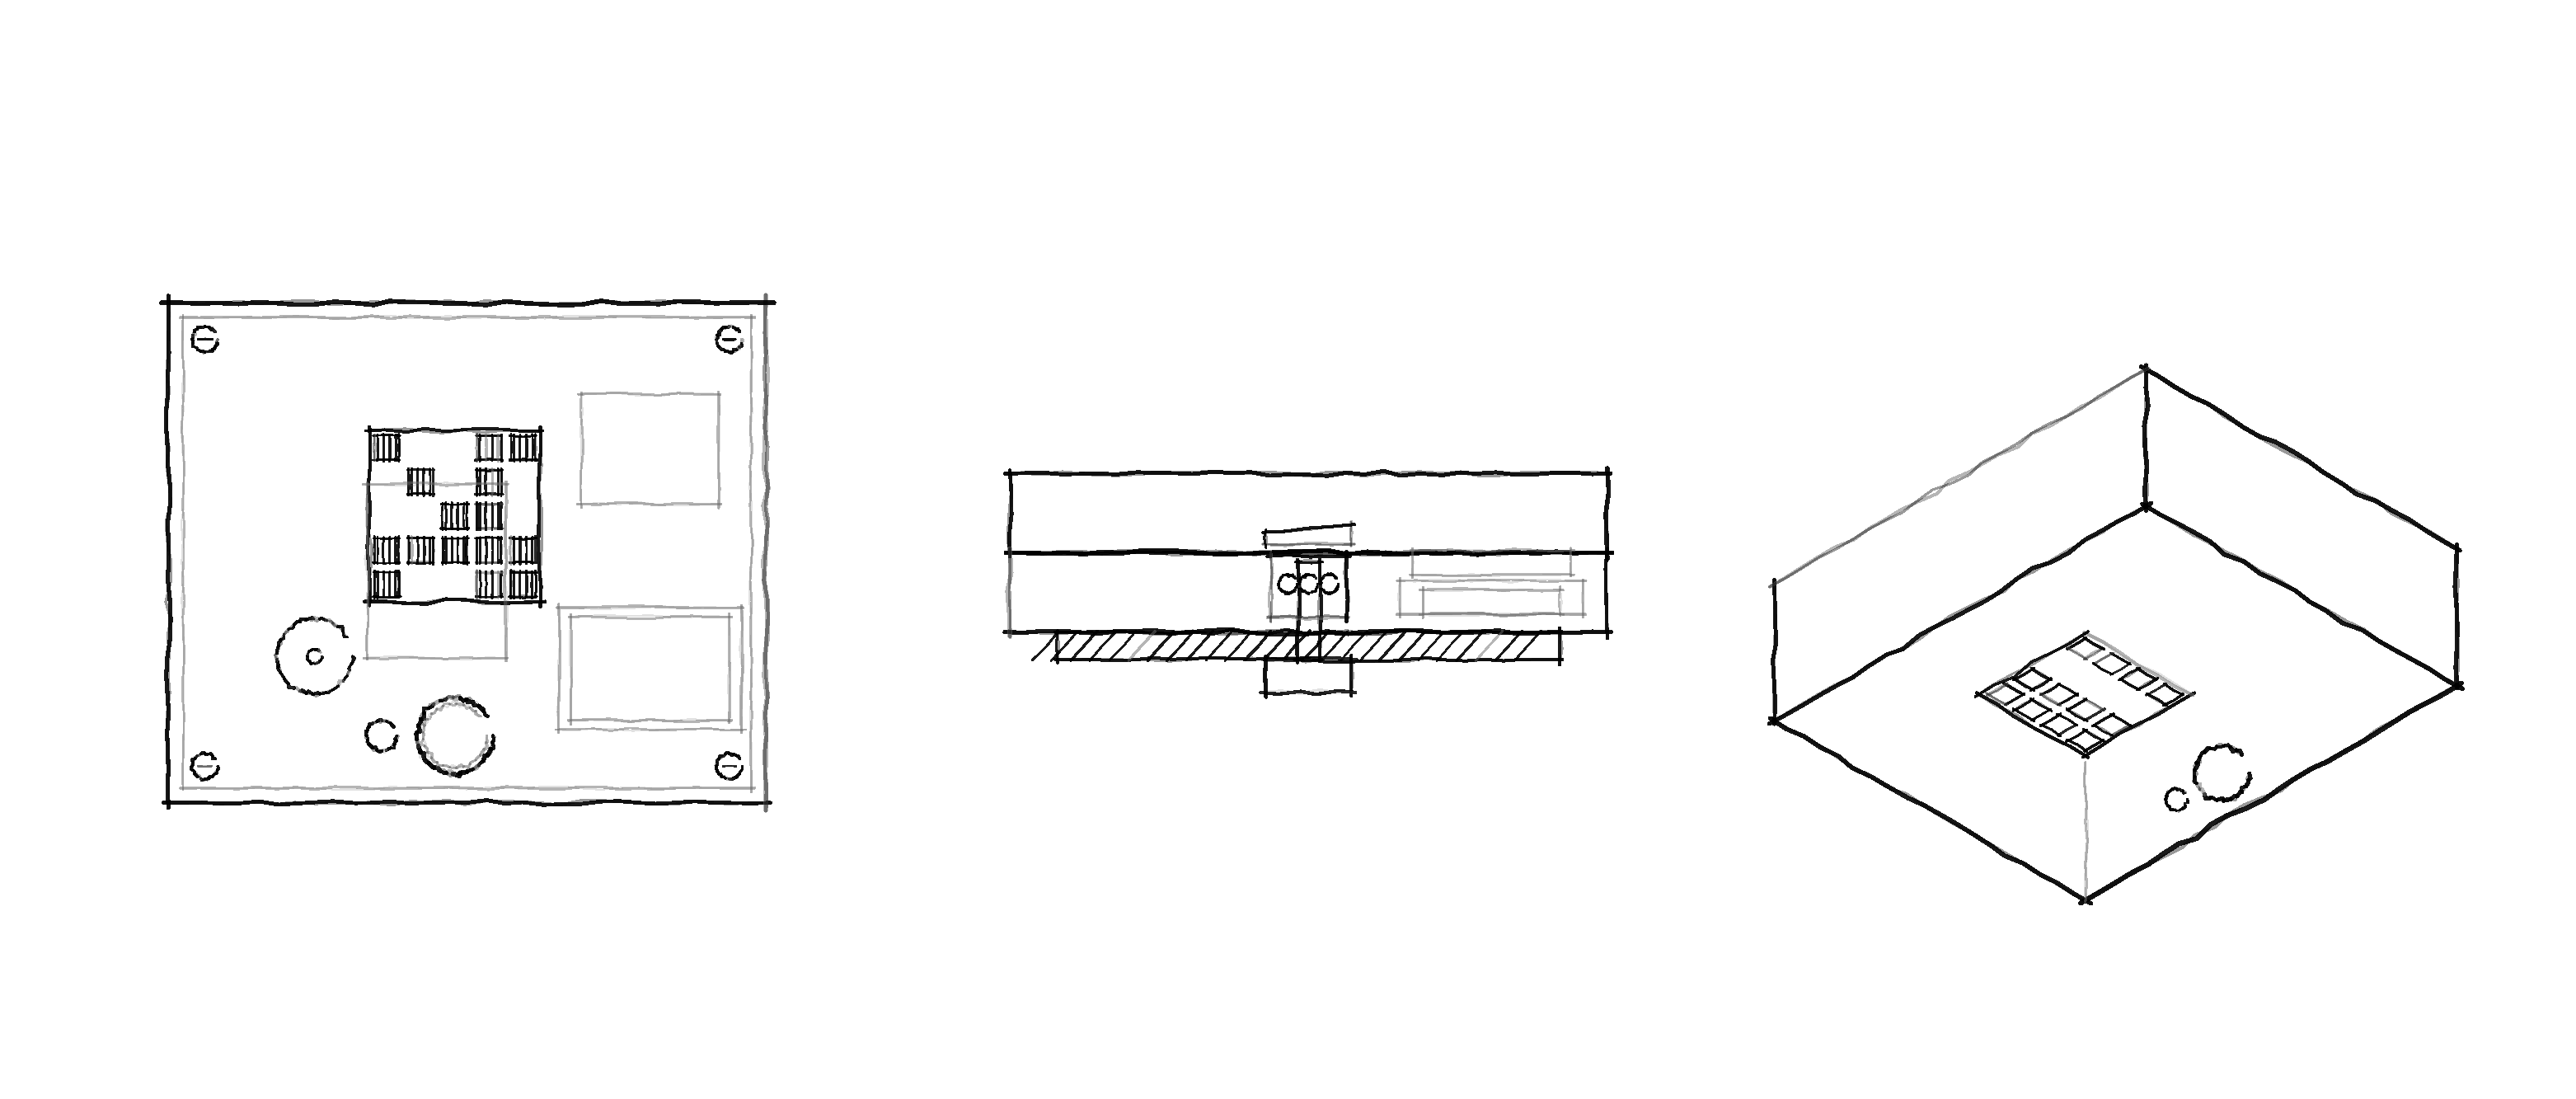
\includegraphics[width=\textwidth]{esboco/escaneado.pdf}
    \label{fig:esboco-mao-livre}
    \source{Elaborado pelos autores (2026).}
\end{figure}

O produto foi concebido como um dispositivo antifurto rígido, de 98\,mm por 82\,mm por 26\,mm, que será preso à peça de roupa da mesma maneira que as etiquetas hoje utilizadas no varejo. Sua face superior concentrará os três elementos de interação com o cliente: um código gráfico impresso, um indicador luminoso e um botão. As dimensões ficaram maiores que as de uma etiqueta convencional porque o dispositivo incorpora bateria, controle e mecanismo de acionamento, isto é, as funções que hoje cabem ao operador do caixa.

\subsection{Funcionamento}
\label{subsec:funcionamento}

A peça de roupa ficará presa por uma haste metálica que atravessa o tecido e penetra o corpo do dispositivo, onde é retida por um mecanismo de garra. O tecido permanece prensado entre a face inferior do dispositivo e o disco da haste, sem perfuração adicional, adesivo ou costura. Como esse é o mesmo princípio das etiquetas convencionais, a compatibilidade com a operação de loja existente fica preservada.

A retenção funciona como uma embreagem de esferas, detalhada na Figura~\ref{fig:esboco-detalhe}. Três esferas de aço são comprimidas contra a haste por um copo cônico, e quanto maior a força aplicada para extraí-la, mais firme fica a retenção. Para liberar a haste, é preciso deslocar o carretel contra a mola que o sustenta. Nas etiquetas convencionais, quem faz isso é o destravador magnético do caixa; no dispositivo proposto, um atuador interno moverá um cursor com rampa, que converte seu deslocamento horizontal em 1,2\,mm de deslocamento vertical aplicado ao carretel.

\begin{figure}[H]
    \centering
    \caption{Detalhe do mecanismo de liberação}
    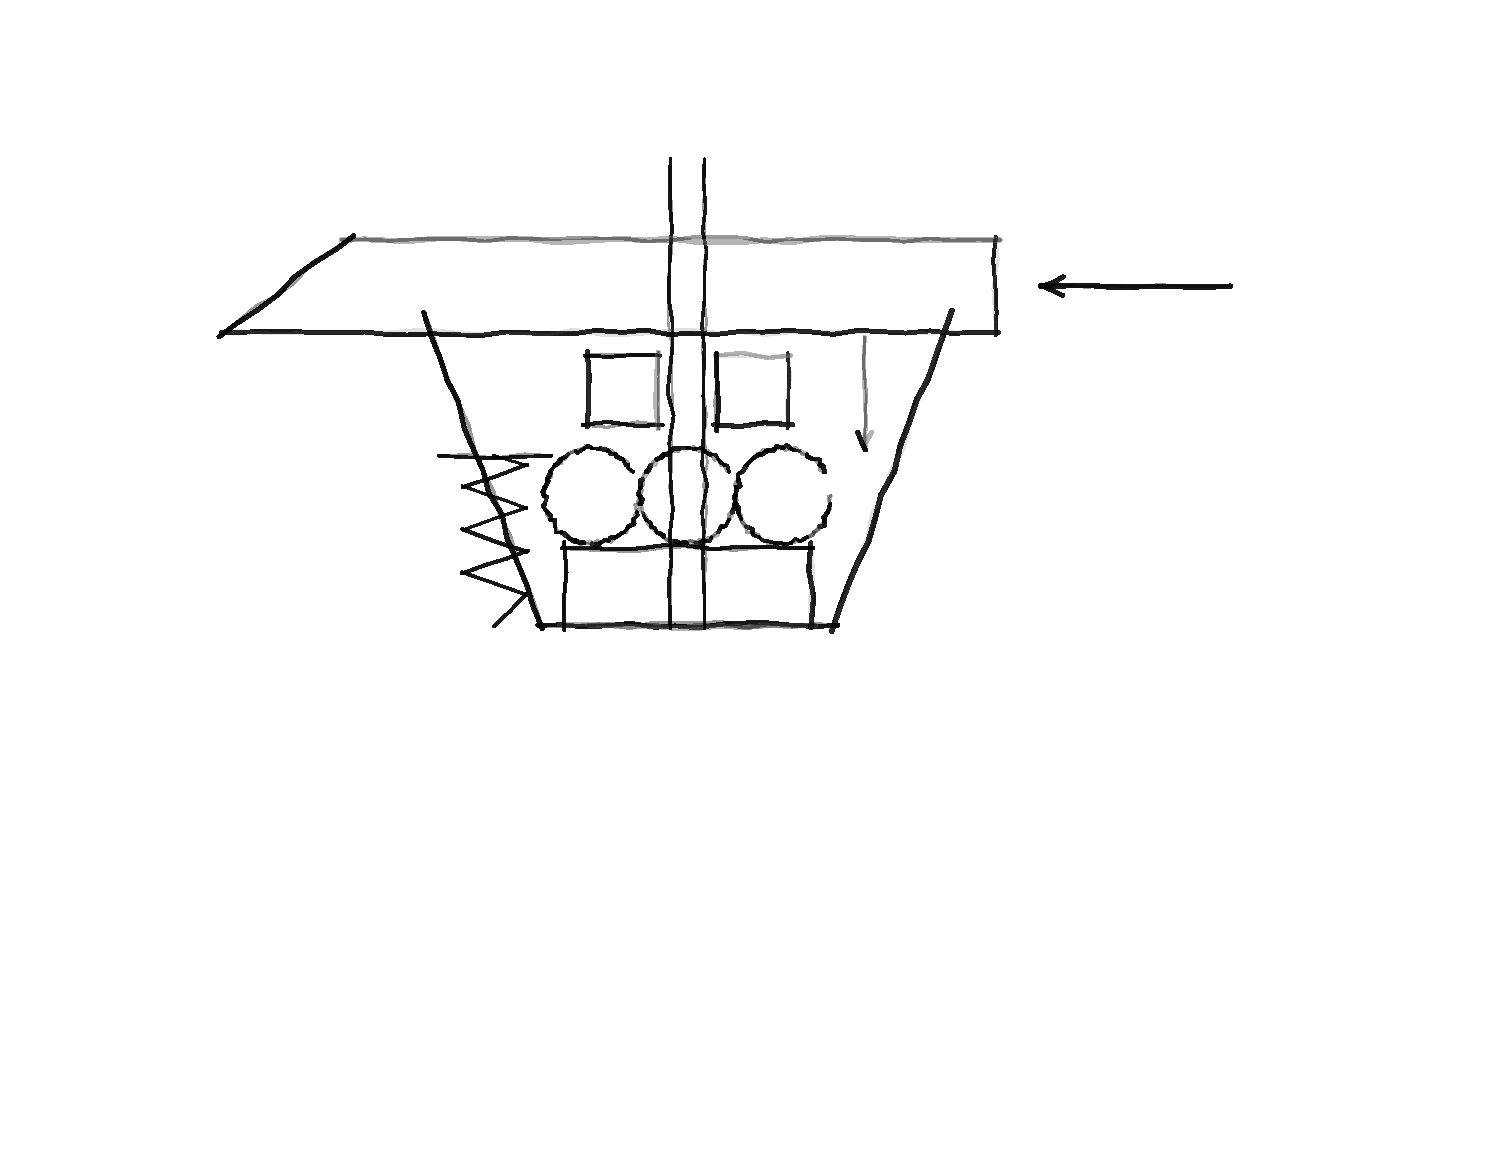
\includegraphics[width=0.8\textwidth]{esboco/escaneado-detalhe.pdf}
    \label{fig:esboco-detalhe}
    \source{Elaborado pelos autores (2026).}
\end{figure}

Com o acionamento passando a ser mecânico, abre-se a possibilidade de tornar o dispositivo imune ao destravador magnético comercial, hoje vendido livremente. Isso dependerá de substituir o carretel por uma peça não ferromagnética, alteração ainda em avaliação.

\subsection{Processo de uso}
\label{subsec:processo_uso}

O consumidor lerá o código impresso com o celular, fará o pagamento no aplicativo e levará a peça ao dispositivo, que receberá a autorização diretamente do aparelho. O indicador passará de vermelho a verde, e o botão liberará a peça. Como a autorização trafega entre o celular e o dispositivo, sem passar pela rede da loja no momento da liberação, uma eventual queda de conexão após o pagamento não impedirá a conclusão da compra.

As dimensões do mecanismo de garra e a escolha do atuador ainda dependem de medições em exemplares comerciais e serão consolidadas na etapa de prototipagem.

\newpage\section{CONSIDERAÇÕES FINAIS}
\textit{[Texto de exemplo --- substituir pelo conteúdo real desta seção.]}
\newpage\section*{REFERÊNCIAS}
\addcontentsline{toc}{section}{REFERÊNCIAS}
\bibliography{bibliografia}

\newpage% =============================================================================
% Anexo A: instrumento completo das entrevistas individuais semiestruturadas
% (projeto Riachuelo, PRO3474).
%
% Documenta o roteiro na ordem em que as perguntas sao feitas ao entrevistado.
% Nao organiza as perguntas em blocos tematicos, nao discute objetivos ou
% hipoteses (isso esta na Secao 6.1, subsec:entrevistas) e nao analisa
% respostas. E apenas o instrumento.
% =============================================================================

\section{Roteiro de entrevista individual semiestruturada}
\label{anexo:roteiro_entrevistas}

Este é o Anexo A do relatório. Documenta o instrumento utilizado nas entrevistas individuais semiestruturadas descritas na Seção~\ref{subsec:entrevistas}. As perguntas aparecem na ordem em que são feitas ao entrevistado, numa sequência única, sem divisão em blocos temáticos. Perguntas de aprofundamento (\textit{probes}) aparecem em itálico, logo após a pergunta principal a que se referem, e o entrevistador as usa apenas quando fizerem sentido na conversa, não como lista fixa. Trechos entre colchetes são instruções de condução, não perguntas a fazer em voz alta. Este anexo apresenta somente o instrumento; a análise das respostas não faz parte deste documento.

\begin{enumerate}
    \item ``Para começar, me conta um pouco sobre como é a sua relação com compra de roupa. Você gosta de comprar, é mais por necessidade, funciona como um passeio?''
    \item ``Com que frequência você compra roupa em loja física, e qual unidade ou região você mais frequenta?''
    \item ``Você costuma comprar mais sozinho(a) ou acompanhado(a)?'' \textit{(Aprofundamento: ``Isso mudou nos últimos anos?'')}
    \item ``Pensa na última vez que você comprou uma peça de roupa numa loja física. Me conta essa história do início ao fim: o que te fez ir à loja, o que aconteceu lá dentro, até você sair.''
    \item ``Nesse momento, você já sabia o que estava procurando, ou foi mais explorando?''
    \item ``Como foi o momento de escolher e experimentar a peça?''
    \item ``E o pagamento, como aconteceu?'' \textit{(Aprofundamento: ``Teve algum momento que você hesitou ou quase desistiu?''; ``Alguma parte demorou mais do que você esperava?''; ``Isso é parecido com o que normalmente acontece pra você, ou foi diferente dessa vez?'')}
    \item ``Quando você está procurando alguma coisa específica numa loja, como você faz para encontrar?''
    \item ``Já aconteceu de você não encontrar o tamanho, a cor ou o modelo que queria?''
    \item ``Você pesquisa em algum canal (site, aplicativo, redes sociais) antes de ir à loja?'' \textit{(Aprofundamento: ``O que você faz quando isso acontece: pede ajuda, procura sozinho por mais tempo, desiste?''; ``Isso te faz sair da loja de mãos vazias com que frequência?''; ``Se você soubesse, antes de sair de casa, que a loja tem o que você quer, isso mudaria alguma coisa em como você compra?'')}
    \item ``Voltando à sua última compra: em algum momento um vendedor te ajudou? Como foi isso?''
    \item ``Tem alguma parte da compra em que você prefere não falar com ninguém e resolver sozinho(a)?''
    \item ``O que um vendedor resolve para você que você não resolveria sozinho?''
    \item ``Já teve uma situação em que a ajuda de um vendedor atrapalhou mais do que ajudou, ou o contrário: sentiu falta de um vendedor e não tinha ninguém por perto?'' \textit{(Aprofundamento: ``Isso muda dependendo do tipo de peça ou do valor?''; ``Isso mudou com o tempo: você busca mais ou menos ajuda hoje do que buscava antes?''; ``Se não tivesse nenhum vendedor disponível na loja inteira, o que você faria diferente?'')}
    \item ``Como foi o momento de pagar na sua última compra? Teve fila?''
    \item ``De modo geral, o que você acha do processo entre decidir que vai levar uma peça e efetivamente sair da loja com ela?''
    \item ``Já desistiu de comprar algo por causa da fila ou da demora no caixa?''
    \item ``O que acontece, na prática, entre você decidir `vou levar isso' e você sair da loja com a peça em mãos?'' \textit{(Aprofundamento: ``Isso acontece com frequência ou foi uma exceção?''; ``O que você faz quando a fila está muito grande: espera, desiste, volta depois?''; ``Alguma vez você sentiu que já tinha `decidido comprar' bem antes de conseguir efetivamente sair da loja com o produto? O que aconteceu nesse meio-tempo?'')}
    \item ``Você já usou algum tipo de autoatendimento (supermercado, farmácia, cinema) sem passar por um funcionário? Como foi?''
    \item ``Você confiaria em pagar por uma peça de roupa pelo celular, sem precisar falar com ninguém na loja?''
    \item ``Como você se sente ao sair de uma loja com uma compra? Já teve alguma experiência desconfortável com alarme, checagem de nota ou verificação na saída?'' \textit{(Aprofundamento: ``O que faria você confiar mais, ou menos, num processo assim?''; ``Isso muda dependendo do valor da peça?'')}
    \item ``Tem alguma coisa sobre comprar roupa em loja física que a gente não conversou e que você acha importante?''
    \item ``Se você pudesse mudar uma única coisa em como as lojas funcionam hoje, o que seria?''
    \item ``Já viu, em outra loja, outro país ou outro tipo de serviço, alguma coisa que resolvesse um problema parecido com os que você mencionou?''
    \item [Retomar, sem repetir de forma idêntica, a pergunta anterior sobre o que o entrevistado mudaria no processo discutido.]
    \item [Descrever o conceito de forma neutra:] ``a Riachuelo está estudando uma etiqueta de segurança na peça que passa a se comunicar com o aplicativo da loja. Ela sabe se a peça foi paga e, quando o pagamento é confirmado pelo aplicativo, ela se destrava sozinha, sem precisar passar pelo caixa.''
    \item [Perguntar a reação livre do entrevistado antes de detalhar qualquer aspecto técnico ou de segurança. Só depois, e apenas se o entrevistado não tocar no assunto espontaneamente, seguir com as perguntas de confiança e segurança abaixo.]
    \item ``O que chama sua atenção nisso, para o bem ou para o mal?''
    \item ``Em que situação você usaria isso, e em que situação não usaria?''
    \item ``Isso resolve algum dos problemas que você mencionou antes, ou resolve outra coisa?''
    \item ``O que precisaria existir, ou o que teria que te garantir, para você confiar nesse processo?''
    \item ``Você entende isso como uma mudança só na trava da peça, ou como algo que muda a experiência de compra como um todo?'' \textit{(Aprofundamento: ``Isso mudaria a forma como você usa o vendedor hoje?''; ``O que te preocuparia mais: a tecnologia falhar, ou perder contato com alguém que te ajuda quando precisa?''; ``Você imagina algum problema com uma peça `saber' que foi manuseada ou onde está dentro da loja?'')}
\end{enumerate}

\newpage% Anexo: Entrevistas individuais completas (PRO3474)
% Transcricao integral das 11 entrevistas semiestruturadas, sem cortes.
% Pressupoe pacote inputenc/utf8 e fontenc T1 no preambulo do documento principal.

\section{Entrevista 1}

\textbf{Danilo:} Para começar, me conta um pouco sobre como é a sua relação com compra de roupa, você gosta de comprar, é mais por necessidade, funciona como um passeio?

\textbf{Marisa:} Ai, eu gosto, viu. Não é só necessidade não. Eu trabalho com venda de doce, fico em casa boa parte do dia, então quando eu saio pra comprar roupa já é tipo um respiro. Gosto de olhar tudo, mexer nas peças, mesmo que eu não vá levar nada... antigamente eu ia mais só pra passear mesmo, hoje em dia geralmente já vou com uma necessidade, tipo repor uma calça do meu marido ou ver alguma coisa pros meus enteados.

\textbf{Danilo:} Com que frequência você compra roupa em loja física, e qual unidade ou região você mais frequenta?

\textbf{Marisa:} Olha, umas duas vezes por mês eu entro numa loja, mas comprar mesmo, levar alguma coisa, é mais tipo uma vez por mês. Eu vou na Renner do Shopping Aricanduva, aqui perto de casa, na Zona Leste. É a que fica mais na mão, porque eu não gosto de pegar muito trânsito, viu.

\textbf{Danilo:} Você costuma comprar mais sozinha ou acompanhada?

\textbf{Marisa:} Ah, quase sempre com minha filha ou com minha sobrinha. Sozinha eu vou mais pra resolver rapidinho, tipo repor uma coisa básica. Mas quando é pra escolher com calma eu gosto de ir acompanhada, elas me ajuda a decidir.

\textbf{Danilo:} Isso mudou nos últimos anos?

\textbf{Marisa:} Mudou sim. Eu ia muito mais antes, quase toda semana dava uma olhada. Hoje eu tô ajudando a cuidar do meu neto, então o tempo ficou mais curto e eu preciso ser mais objetiva quando vou, né.

\textbf{Danilo:} Pensa na última vez que você comprou uma peça de roupa numa loja física. Me conta essa história do início ao fim, o que te fez ir à loja, o que aconteceu lá dentro, até você sair.

\textbf{Marisa:} Foi semana passada. Eu fui porque a calça do meu marido rasgou e ele precisava de uma pra trabalhar ainda naquela semana... deixa eu ver, foi numa terça, acho, ou quarta, não lembro direito. Cheguei lá, a loja tava bem cheia, tinha promoção de inverno. Fiquei um tempo procurando sozinha, não achei o tamanho dele na cor que eu queria, aí chamei uma moça que trabalha lá, ela é bem atenciosa, sabe, já me atendeu outras vezes. Ela foi no estoque e trouxe em outra cor, serviu bem. Aí de passagem eu vi uma blusa bonita pra mim, acabei provando também, gostei e levei. Paguei no cartão de débito e fui embora.

\textbf{Danilo:} Nesse momento, você já sabia o que estava procurando, ou foi mais explorando?

\textbf{Marisa:} Da calça eu sabia certinho, o número, a cor que ele gosta. Mas a blusa foi mais porque eu vi passando mesmo, não tava nos meus planos não.

\textbf{Danilo:} Como foi o momento de escolher e experimentar a peça?

\textbf{Marisa:} A calça eu nem provei, é dele, eu só confio no tamanho. Já a blusa eu experimentei no provador, mas tava com fila, tive que esperar um pouco pra vagar uma cabine.

\textbf{Danilo:} E o pagamento, como aconteceu?

\textbf{Marisa:} No caixa, cartão de débito, rapidinho, mas antes de chegar lá teve uma filazinha, coisa de uns dez minutos.

\textbf{Danilo:} Teve algum momento que você hesitou ou quase desistiu?

\textbf{Marisa:} Hesitei no preço da calça, tava mais caro do que eu lembrava. Mas como ele precisava mesmo, levei assim.

\textbf{Danilo:} Alguma parte demorou mais do que você esperava?

\textbf{Marisa:} O provador. Tinha só duas cabine abertas e uma fila de umas quatro pessoas.

\textbf{Danilo:} Isso é parecido com o que normalmente acontece pra você, ou foi diferente dessa vez?

\textbf{Marisa:} É bem parecido, viu. Quase sempre que eu vou tem fila de provador, principalmente fim de semana.

\textbf{Danilo:} Quando você está procurando alguma coisa específica numa loja, como você faz para encontrar?

\textbf{Marisa:} Eu ando pelos corredor olhando, mas confesso que às vezes eu fico meio perdida, a loja é grande e muda os produto de lugar. Se eu não acho rápido, eu já chamo alguém pra me ajudar, não fico procurando muito tempo sozinha não.

\textbf{Danilo:} Já aconteceu de você não encontrar o tamanho, a cor ou o modelo que queria?

\textbf{Marisa:} Demais. Principalmente pra mim mesma, que eu uso um tamanho que sempre falta. Isso é bem frequente, viu.

\textbf{Danilo:} Você pesquisa em algum canal, site, aplicativo, redes sociais, antes de ir à loja?

\textbf{Marisa:} Não, quase nunca. Eu não sou muito boa com essas aplicativo, prefiro ir direto e ver pessoalmente.

\textbf{Danilo:} O que você faz quando isso acontece, pede ajuda, procura sozinha por mais tempo, desiste?

\textbf{Marisa:} Peço ajuda quase sempre. Se não tem ninguém disponível, aí eu deixo pra outro dia.

\textbf{Danilo:} Isso te faz sair da loja de mãos vazias com que frequência?

\textbf{Marisa:} De vez em quando acontece, não é toda vez, mas acontece.

\textbf{Danilo:} Se você soubesse, antes de sair de casa, que a loja tem o que você quer, isso mudaria alguma coisa em como você compra?

\textbf{Marisa:} Mudaria bastante, viu. Eu ia direto sem ficar rodando à toa, porque às vezes eu vou, não acho, e tenho que ir embora sem nada, e isso é um saco.

\textbf{Danilo:} Voltando à sua última compra, em algum momento um vendedor te ajudou? Como foi isso?

\textbf{Marisa:} Ajudou, sim, já contei, a moça foi buscar a calça no estoque pra mim. Se não fosse ela eu tinha saído sem levar.

\textbf{Danilo:} Tem alguma parte da compra em que você prefere não falar com ninguém e resolver sozinha?

\textbf{Marisa:} Na hora de experimentar eu prefiro ficar sozinha no provedor, não gosto que fiquem esperando do lado, me sinto pressionada.

\textbf{Danilo:} O que um vendedor resolve para você que você não resolveria sozinha?

\textbf{Marisa:} Achar tamanho que não tá na araque, e também dar uma opinião se ficou bom em mim, porque às vezes eu mesma não confio no meu julgamento não.

\textbf{Danilo:} Já teve uma situação em que a ajuda de um vendedor atrapalhou mais do que ajudou, ou o contrário, sentiu falta de um vendedor e não tinha ninguém por perto?

\textbf{Marisa:} Já teve vez de eu precisar e não achar ninguém, aí eu esperei um bom tempo parada num corredor até alguém passar. Isso me deixou incomodada, viu.

\textbf{Danilo:} Isso muda dependendo do tipo de peça ou do valor?

\textbf{Marisa:} Muda. Pra coisa mais cara eu quero mais atenção, quero ter certeza que eu tô fazendo a escolha certa.

\textbf{Danilo:} Isso mudou com o tempo, você busca mais ou menos ajuda hoje do que buscava antes?

\textbf{Marisa:} Acho que busco mais hoje. Com a idade eu confio menos na minha vista pra ver se caiu bem, aí prefiro perguntar.

\textbf{Danilo:} Como foi o momento de pagar na sua última compra? Teve fila?

\textbf{Marisa:} Teve, uns dez minuto, não foi terrível mas também não foi rápido.

\textbf{Danilo:} De modo geral, o que você acha do processo entre decidir que vai levar uma peça e efetivamente sair da loja com ela?

\textbf{Marisa:} Acho meio demorado, mas eu já acostumei que é assim mesmo. Não é uma coisa que me revolta, entende, é mais uma coisa que eu já espero que aconteça.

\textbf{Danilo:} Já desistiu de comprar algo por causa da fila ou da demora no caixa?

\textbf{Marisa:} Uma vez, no fim de ano, a fila tava enorme e eu desisti, devolvi a peça na araque e fui embora.

\textbf{Danilo:} O que acontece, na prática, entre você decidir vou levar isso e você sair da loja com a peça em mãos?

\textbf{Marisa:} Eu ando até o caixa, geralmente tem fila, fico esperando, às vezes converso com quem tá do lado, e depois pago e vou.

\textbf{Danilo:} Isso acontece com frequência ou foi uma exceção?

\textbf{Marisa:} Mais em data de fim de ano e promoção. No dia a dia é mais tranquilo.

\textbf{Danilo:} Você já usou algum tipo de autoatendimento, supermercado, farmácia, cinema, sem passar por um funcionário? Como foi?

\textbf{Marisa:} Já usei o caixa de autoatendimento do mercado, mas não gosto muito não, prefiro caixa com pessoa. Fico com medo de errar alguma coisa na máquina e ninguém perceber.

\textbf{Danilo:} Você confiaria em pagar por uma peça de roupa pelo celular, sem precisar falar com ninguém na loja?

\textbf{Marisa:} Acho que não, não muito. Tenho medo de ser cobrada duas vez ou de dar algum erro e eu não saber resolver sozinha.

\textbf{Danilo:} Como você se sente ao sair de uma loja com uma compra, já teve alguma experiência desconfortável com alarme, checagem de nota ou verificação na saída?

\textbf{Marisa:} Já sim, uma vez o alarme disparou sem motivo, foi bem sem graça, todo mundo olhando. Eu tinha pago certinho mas fiquei super encabulada.

\textbf{Danilo:} O que faria você confiar mais, ou menos, num processo assim?

\textbf{Marisa:} Confiaria mais se soubesse que tem alguém pra me ajudar caso desse algum problema. Sozinha eu fico insegura.

\textbf{Danilo:} Tem alguma coisa sobre comprar roupa em loja física que a gente não conversou e que você acha importante?

\textbf{Marisa:} Acho que o provador é uma coisa que pesa bastante, viu. Poucas cabine, fila grande, isso atrapalha demais, principalmente em dia de promoção.

\textbf{Danilo:} Se você pudesse mudar uma única coisa em como as lojas funcionam hoje, o que seria?

\textbf{Marisa:} Colocaria mais vendedora e mais provador nos dias de promoção, que é quando mais precisa.

\textbf{Danilo:} Já viu, em outra loja, outro país ou outro tipo de serviço, alguma coisa que resolvesse um problema parecido com os que você mencionou?

\textbf{Marisa:} Não muito, não. Lembro de antigamente ter caderneta de fiado em loja pequena, mas isso é outra história, não tem nada a ver com isso que você tá perguntando.

\textbf{Danilo:} Voltando no que você comentou sobre faltar vendedora e provador nos dias cheios, a Riachuelo está estudando uma etiqueta de segurança na peça que passa a se comunicar com o aplicativo da loja. Ela sabe se a peça foi paga e, quando o pagamento é confirmado pelo aplicativo, ela se destrava sozinha, sem precisar passar pelo caixa. O que chama sua atenção nisso, para o bem ou para o mal?

\textbf{Marisa:} Olha, eu fico com um pé atrás, viu. Fico pensando, e se der algum erro e a etiqueta não destravar, ou pior, destravar errado e eu ser acusada de estar levando sem pagar? Isso me preocupa mais do que me anima, sinceramente.

\textbf{Danilo:} Em que situação você usaria isso, e em que situação não usaria?

\textbf{Marisa:} Acho que só usaria se tivesse uma vendedora por perto pra confirmar que deu certo. Sozinha, sem ninguém, eu não confiaria não.

\textbf{Danilo:} Isso resolve algum dos problemas que você mencionou antes, ou resolve outra coisa?

\textbf{Marisa:} Não resolve o que eu mais reclamei, que é falta de vendedora e de provador. Isso aqui é outra coisa, é mais sobre a fila do caixa, que pra mim nem é o que mais incomoda.

\textbf{Danilo:} O que precisaria existir, ou o que teria que te garantir, para você confiar nesse processo?

\textbf{Marisa:} Precisava ter uma garantia bem clara de que não vai dar problema, e alguém pra eu recorrer caso desse.

\textbf{Danilo:} O que te preocuparia mais, a tecnologia falhar, ou perder contato com alguém que te ajuda quando precisa?

\textbf{Marisa:} Perder o contato com quem ajuda, com certeza. Pra mim isso é mais importante que a tecnologia funcionar direitinho.


\section{Entrevista 2}

\textbf{Mateus:} Para começar, me conta um pouco sobre como é a sua relação com compra de roupa, você gosta de comprar, é mais por necessidade, funciona como um passeio?

\textbf{Joyce:} É mais necessidade mesmo, sinceramente. Trabalho o dia inteiro, tenho meu filho pequeno, então quando eu vou numa loja já é porque precisa mesmo, roupa dele que ficou pequena ou uma coisa minha que rasgou.

\textbf{Mateus:} Com que frequência você compra roupa em loja física, e qual unidade ou região você mais frequenta?

\textbf{Joyce:} Umas duas, três semana eu dou uma passada, sempre na Renner do Shopping Interlagos, aqui perto, na Zona Sul. É onde eu pego meu filho na escola, então já aproveito o caminho.

\textbf{Mateus:} Você costuma comprar mais sozinha ou acompanhada?

\textbf{Joyce:} Sozinha, na maioria das vezes. Às vezes levo meu filho junto, mas contando ele não como companhia, tipo, mais como responsabilidade extra.

\textbf{Mateus:} Isso mudou nos últimos anos?

\textbf{Joyce:} Mudou bastante depois que ele nasceu. Antes eu ia com mais calma, hoje é tudo correndo, entro, resolvo e saio.

\textbf{Mateus:} Pensa na última vez que você comprou uma peça de roupa numa loja física. Me conta essa história do início ao fim, o que te fez ir à loja, o que aconteceu lá dentro, até você sair.

\textbf{Joyce:} Foi tipo duas semana atrás. Fui comprar um casaco pro meu filho porque tava esfriando e ele não tinha nada quentinho. Cheguei, fui direto na seção infantil, já sabia mais ou menos o que queria, achei rápido, provei nele ali mesmo, coloquei o casaco e vi que servia, e fui pagar.

\textbf{Mateus:} Me dá um exemplo de como foi essa parte de achar o casaco, foi tranquilo mesmo?

\textbf{Joyce:} Foi, porque eu fui num dia de semana de manhã, loja meio vazia. Achei umas três opção de cor, escolhi a mais neutra, testei nele e já resolvi.

\textbf{Mateus:} Nesse momento, você já sabia o que estava procurando, ou foi mais explorando?

\textbf{Joyce:} Sabia certinho, casaco, tamanho dele, não tinha muito tempo pra ficar olhando outra coisa.

\textbf{Mateus:} Como foi o momento de escolher e experimentar a peça?

\textbf{Joyce:} Rápido, testei nele ali mesmo no corredor, nem fui no provador porque não tinha necessidade.

\textbf{Mateus:} E o pagamento, como aconteceu?

\textbf{Joyce:} Paguei no cartão, no aplicativo do banco mesmo, por aproximação. Não teve fila porque era horário fraco.

\textbf{Mateus:} Teve algum momento que você hesitou ou quase desistiu?

\textbf{Joyce:} Não, dessa vez não. Foi tranquilo.

\textbf{Mateus:} Alguma parte demorou mais do que você esperava?

\textbf{Joyce:} Não, foi rápido, uns quinze minuto do início ao fim.

\textbf{Mateus:} Isso é parecido com o que normalmente acontece pra você, ou foi diferente dessa vez?

\textbf{Joyce:} Foi mais tranquilo que o normal, porque geralmente eu vou fim de semana, que é quando dá pra eu ter mais tempo, e aí tem mais gente.

\textbf{Mateus:} Quando você está procurando alguma coisa específica numa loja, como você faz para encontrar?

\textbf{Joyce:} Eu ando pelas seção, já tenho noção de onde fica cada coisa porque eu vou sempre na mesma loja. Se não acho eu procuro alguém rapidinho, mas prefiro tentar sozinha primeiro.

\textbf{Mateus:} Já aconteceu de você não encontrar o tamanho, a cor ou o modelo que queria?

\textbf{Joyce:} Já, principalmente roupa de criança em tamanho específico, eles vende muito rápido.

\textbf{Mateus:} Você pesquisa em algum canal, site, aplicativo, redes sociais, antes de ir à loja?

\textbf{Joyce:} Às vezes eu dou uma olhada no site antes, mas não confio cem por cento que o que tá lá vai estar na loja de verdade. Aí eu vou mesmo assim conferir pessoalmente.

\textbf{Mateus:} Conta mais sobre isso, por que você não confia que o que tá no site vai estar na loja?

\textbf{Joyce:} Porque já aconteceu de eu ver uma coisa disponível no site e chegar lá e não achar, aí acabei desconfiando, sabe. Prefiro ir olhar com meus próprios olho.

\textbf{Mateus:} O que você faz quando isso acontece, pede ajuda, procura sozinha por mais tempo, desiste?

\textbf{Joyce:} Pergunto pra alguém, se não tiver ninguém e eu tiver com pressa, que é o mais comum, eu desisto e vou embora, não tenho tempo de ficar esperando não.

\textbf{Mateus:} Isso te faz sair da loja de mãos vazias com que frequência?

\textbf{Joyce:} De vez em quando, tipo uma vez por mês isso acontece.

\textbf{Mateus:} Se você soubesse, antes de sair de casa, que a loja tem o que você quer, isso mudaria alguma coisa em como você compra?

\textbf{Joyce:} Mudaria muito, porque eu tenho pouco tempo, se eu já soubesse que tem, eu ia direto sem perder tempo procurando.

\textbf{Mateus:} Voltando à sua última compra, em algum momento um vendedor te ajudou? Como foi isso?

\textbf{Joyce:} Não precisei dessa vez, resolvi tudo sozinha.

\textbf{Mateus:} Tem alguma parte da compra em que você prefere não falar com ninguém e resolver sozinha?

\textbf{Joyce:} Praticamente tudo, na verdade. Eu gosto de resolver rápido sem precisar ficar explicando o que eu quero pra alguém.

\textbf{Mateus:} O que um vendedor resolve para você que você não resolveria sozinha?

\textbf{Joyce:} Quando não acho um tamanho na araque, aí eu preciso perguntar se tem no estoque.

\textbf{Mateus:} Já teve uma situação em que a ajuda de um vendedor atrapalhou mais do que ajudou, ou o contrário, sentiu falta de um vendedor e não tinha ninguém por perto?

\textbf{Joyce:} Já senti falta sim, uma vez eu precisava de um tamanho e não achei ninguém por dez minuto, isso me irritou porque eu tava com pressa.

\textbf{Mateus:} Isso muda dependendo do tipo de peça ou do valor?

\textbf{Joyce:} Um pouco. Pra roupa de criança eu me importo mais em achar rápido, pra roupa minha eu até gosto de olhar mais com calma quando dá tempo.

\textbf{Mateus:} Como foi o momento de pagar na sua última compra? Teve fila?

\textbf{Joyce:} Não teve fila dessa vez, mas geralmente tem, principalmente fim de semana.

\textbf{Mateus:} De modo geral, o que você acha do processo entre decidir que vai levar uma peça e efetivamente sair da loja com ela?

\textbf{Joyce:} Acho que podia ser mais rápido. Pra quem tem pouco tempo como eu, cada minuto de fila pesa.

\textbf{Mateus:} Já desistiu de comprar algo por causa da fila ou da demora no caixa?

\textbf{Joyce:} Já, mais de uma vez. Se a fila tá enorme e eu tenho hora pra buscar meu filho, eu devolvo a peça e vou embora.

\textbf{Mateus:} Me conta de uma vez específica que isso aconteceu.

\textbf{Joyce:} Foi num sábado, eu tava com uma blusa escolhida, vi a fila do caixa enorme, olhei no relógio, vi que ia atrasar, e simplesmente deixei a peça numa araque perto e saí.

\textbf{Mateus:} O que acontece, na prática, entre você decidir vou levar isso e você sair da loja com a peça em mãos?

\textbf{Joyce:} Eu ando até o caixa, olho o tamanho da fila, se for rápido eu fico, se não for eu já penso duas vez.

\textbf{Mateus:} Isso acontece com frequência ou foi uma exceção?

\textbf{Joyce:} Acontece bastante, principalmente fim de semana e data comemorativa.

\textbf{Mateus:} Você já usou algum tipo de autoatendimento, supermercado, farmácia, cinema, sem passar por um funcionário? Como foi?

\textbf{Joyce:} Uso direto no mercado, autoatendimento, acho ótimo, bem mais rápido.

\textbf{Mateus:} Você confiaria em pagar por uma peça de roupa pelo celular, sem precisar falar com ninguém na loja?

\textbf{Joyce:} Confiaria, eu já uso pix e cartão pelo celular pra tudo, não vejo muito problema nisso não.

\textbf{Mateus:} Como você se sente ao sair de uma loja com uma compra, já teve alguma experiência desconfortável com alarme, checagem de nota ou verificação na saída?

\textbf{Joyce:} Nunca tive problema com alarme, mas às vezes acho chato ter que mostrar a nota na saída, parece que estão desconfiando de mim.

\textbf{Mateus:} O que faria você confiar mais, ou menos, num processo assim?

\textbf{Joyce:} Confiaria mais se fosse rápido e não desse trabalho, tipo, se eu não precisasse ficar mostrando nada pra ninguém.

\textbf{Mateus:} Tem alguma coisa sobre comprar roupa em loja física que a gente não conversou e que você acha importante?

\textbf{Joyce:} Acho que falta mais opção de horário com loja mais vazia. Eu queria poder ir de manhã cedo sempre, mas nem sempre dá.

\textbf{Mateus:} Se você pudesse mudar uma única coisa em como as lojas funcionam hoje, o que seria?

\textbf{Joyce:} Deixaria o caixa mais rápido, com menos gente na frente.

\textbf{Mateus:} Já viu, em outra loja, outro país ou outro tipo de serviço, alguma coisa que resolvesse um problema parecido com os que você mencionou?

\textbf{Joyce:} Vi um mercado aqui perto que tem uns totem de autoatendimento bem rápido, gostaria que loja de roupa tivesse algo assim também.

\textbf{Mateus:} Você comentou que gostaria de um jeito mais rápido de pagar, sem tanta fila. A Riachuelo está estudando uma etiqueta de segurança na peça que passa a se comunicar com o aplicativo da loja. Ela sabe se a peça foi paga e, quando o pagamento é confirmado pelo aplicativo, ela se destrava sozinha, sem precisar passar pelo caixa. O que chama sua atenção nisso, para o bem ou para o mal?

\textbf{Joyce:} Achei interessante, principalmente pra quando eu tô com pressa. Se funcionar direito, resolveria bastante coisa pra mim.

\textbf{Mateus:} Em que situação você usaria isso, e em que situação não usaria?

\textbf{Joyce:} Usaria em qualquer compra rápida, tipo roupa básica. Talvez não usasse se fosse alguma coisa mais cara, aí eu ia querer ter certeza de que deu tudo certo antes de sair.

\textbf{Mateus:} Isso resolve algum dos problemas que você mencionou antes, ou resolve outra coisa?

\textbf{Joyce:} Resolve bem o problema da fila, que é o que mais me incomoda. Não resolve o problema de achar tamanho, mas pelo menos essa parte ajudaria.

\textbf{Mateus:} O que precisaria existir, ou o que teria que te garantir, para você confiar nesse processo?

\textbf{Joyce:} Precisava mostrar bem claro no aplicativo que o pagamento foi confirmado, algum aviso, tipo pode sair, tá tudo certo.

\textbf{Mateus:} Você entende isso como uma mudança só na trava da peça, ou como algo que muda a experiência de compra como um todo?

\textbf{Joyce:} Acho que muda mais a parte de sair rápido da loja. O resto, achar produto, provar, continua igual.

\textbf{Mateus:} Isso mudaria a forma como você usa o vendedor hoje?

\textbf{Joyce:} Não muito, eu já uso pouco vendedor mesmo, então continuaria mais ou menos igual.


\section{Entrevista 3}

\textbf{Lucas:} E aí, Robério, bora começar. Me conta um pouco, como é a sua relação com compra de roupa? Você gosta, é mais por necessidade, é tipo um passeio?

\textbf{Robério:} Ah, é mais necessidade mesmo. Eu não sou muito de sair pra comprar roupa por diversão não. Quando eu vou é porque precisa.

\textbf{Lucas:} Com que frequência você compra, e onde costuma ir?

\textbf{Robério:} Poucas vez, viu. Umas três, quatro vez por ano. Vou na C\&A do Shopping Cidade Sorocaba mesmo, perto de casa.

\textbf{Lucas:} E costuma ir sozinho ou acompanhado?

\textbf{Robério:} Geralmente com minha esposa. Ela que me ajuda a escolher, porque sozinho eu me perco um pouco.

\textbf{Lucas:} Isso mudou nos últimos anos?

\textbf{Robério:} Mudou. Antes eu ia mais, trabalhava, precisava de roupa pra semana toda. Aposentei, aí ficou bem mais raro.

\textbf{Lucas:} Beleza. Agora pensa na última vez que você comprou uma roupa numa loja física. Me conta essa história inteira, desde o que te fez ir até você sair de lá.

\textbf{Robério:} Foi acho que uns dois mês atrás. Minha esposa que me levou, precisava de uma camisa pra um casamento. A gente foi, ela que escolheu umas opção, eu só fui provando o que ela trazia.

\textbf{Lucas:} E você já sabia o que queria, ou foi mais ela que foi guiando?

\textbf{Robério:} Foi ela que guiou, eu não entendo muito dessas coisa de moda não.

\textbf{Lucas:} Como foi a parte de experimentar?

\textbf{Robério:} Fui no provador, ela ficava esperando do lado de fora, ia passando as opção.

\textbf{Lucas:} E o pagamento, como foi?

\textbf{Robério:} No caixa, no cartão. Teve uma filazinha, mas nada absurdo.

\textbf{Lucas:} Teve algum momento que você hesitou ou quase desistiu?

\textbf{Robério:} Hesitei no preço, achei meio caro, mas como era pra ocasião especial, levei.

\textbf{Lucas:} Alguma parte demorou mais do que esperava?

\textbf{Robério:} Não, foi tranquilo, uns quarenta minuto no total.

\textbf{Lucas:} E isso é parecido com o que normalmente rola, ou foi diferente?

\textbf{Robério:} É parecido. Eu não vou com muita frequência, mas quando vou é sempre assim, minha esposa na frente decidindo e eu ajudando pouco, viu.

\textbf{Lucas:} Quando você procura alguma coisa específica, como você faz pra achar?

\textbf{Robério:} Eu mesmo não procuro muito não, prefiro perguntar pra alguém da loja logo de cara.

\textbf{Lucas:} Já aconteceu de não achar o tamanho ou modelo que queria?

\textbf{Robério:} Já, sim. Às vezes o tamanho que eu uso já tinha acabado.

\textbf{Lucas:} Você pesquisa em site ou aplicativo antes de ir?

\textbf{Robério:} Não, isso eu não mexo. Nem tenho muita paciência pra essas coisa de celular, viu.

\textbf{Lucas:} E quando não acha o que quer, o que você faz? Pede ajuda, procura mais, desiste?

\textbf{Robério:} Peço ajuda pra minha esposa primeiro, e se ela não resolver a gente chama alguém da loja.

\textbf{Lucas:} Isso faz você sair de mãos vazias com que frequência?

\textbf{Robério:} De vez em quando acontece, mas não é o mais comum não.

\textbf{Lucas:} Se você soubesse antes que a loja tem o que você quer, isso mudaria alguma coisa?

\textbf{Robério:} Mudaria, porque eu não gosto de ir à toa. Se eu soubesse que não tem, nem ia.

\textbf{Lucas:} Voltando pra última compra, um vendedor te ajudou em algum momento?

\textbf{Robério:} Ajudou sim, minha esposa chamou uma moça pra trazer outro tamanho.

\textbf{Lucas:} Tem alguma parte que você prefere resolver sozinho, sem falar com ninguém?

\textbf{Robério:} Olha, eu prefiro que tenha sempre alguém por perto, viu. Não gosto muito de ficar resolvendo essas coisa sozinho.

\textbf{Lucas:} O que um vendedor resolve pra você que você não resolveria sozinho?

\textbf{Robério:} Quase tudo, sinceramente. Escolher, saber se ficou bom, achar tamanho. Eu confio mais neles do que em mim mesmo nessas hora.

\textbf{Lucas:} Já teve alguma vez que a ajuda atrapalhou, ou o contrário, sentiu falta e não tinha ninguém?

\textbf{Robério:} Já senti falta, uma vez fiquei um tempo esperando alguém aparecer e fiquei sem graça de ficar ali parado.

\textbf{Lucas:} Isso muda dependendo da peça ou do valor?

\textbf{Robério:} Acho que não muda muito não, eu sempre prefiro ter ajuda, seja coisa cara ou barata.

\textbf{Lucas:} E mudou com o tempo? Você busca mais ou menos ajuda hoje?

\textbf{Robério:} Acho que sempre busquei bastante, não mudou muito não.

\textbf{Lucas:} Se não tivesse nenhum vendedor na loja inteira, o que você faria diferente?

\textbf{Robério:} Acho que eu ia embora sem comprar, viu. Não ia me sentir seguro de escolher sozinho não.

\textbf{Lucas:} Como foi o pagamento na sua última compra? Teve fila?

\textbf{Robério:} Teve uma filazinha pequena, nada demorado.

\textbf{Lucas:} De modo geral, o que você acha desse processo entre decidir levar a peça e sair da loja?

\textbf{Robério:} Acho normal, não me incomoda muito não. Pra mim o que mais demora é a escolha mesmo, não o pagamento.

\textbf{Lucas:} Já desistiu de comprar algo por causa da fila?

\textbf{Robério:} Não, nunca desisti por causa disso.

\textbf{Lucas:} O que acontece, na prática, entre você decidir vou levar isso e sair da loja com a peça?

\textbf{Robério:} Vou até o caixa, espero a vez, pago e saio. É bem direto pra mim.

\textbf{Lucas:} Você já usou algum tipo de autoatendimento, tipo mercado ou farmácia, sem passar por funcionário?

\textbf{Robério:} Já vi tendo em mercado, mas eu mesmo prefiro sempre o caixa com pessoa. Não confio muito nessas máquina não.

\textbf{Lucas:} Você confiaria em pagar por uma roupa pelo celular, sem falar com ninguém na loja?

\textbf{Robério:} Não, isso eu não confiaria muito não. Prefiro ter uma pessoa por perto pra garantir que tá tudo certo.

\textbf{Lucas:} Já teve alguma experiência desconfortável com alarme ou checagem na saída?

\textbf{Robério:} Não, nunca tive problema desse tipo.

\textbf{Lucas:} O que faria você confiar mais, ou menos, num processo assim?

\textbf{Robério:} Confiaria mais se tivesse sempre alguém que eu pudesse perguntar se desse algum problema.

\textbf{Lucas:} Tem alguma coisa sobre comprar roupa que a gente não conversou e você acha importante?

\textbf{Robério:} Acho que já falamos do principal, que é eu gostar de ter gente que ajude.

\textbf{Lucas:} Se pudesse mudar uma coisa só nas lojas hoje, o que seria?

\textbf{Robério:} Colocaria mais gente pra atender, principalmente perto do provador.

\textbf{Lucas:} Já viu em outro lugar alguma coisa parecida que resolvesse algum desses problemas?

\textbf{Robério:} Não, não vi não. Eu não saio muito, nem presto muita atenção nessas coisa não.

\textbf{Lucas:} Legal. Deixa eu te falar de uma ideia que a Riachuelo tá estudando, uma etiqueta de segurança na peça que se comunica com o aplicativo da loja. Ela sabe se a peça foi paga, e quando o pagamento é confirmado pelo aplicativo, ela se destrava sozinha, sem precisar passar pelo caixa. O que você acha disso, pra bem ou pra mal?

\textbf{Robério:} Ah, isso me deixa bem inseguro, viu. Eu nem uso muito celular pra essas coisa, imagina pagar sozinho e confiar que vai destravar certo.

\textbf{Lucas:} Em que situação você usaria isso, e em que não usaria?

\textbf{Robério:} Acho que eu não usaria em quase nenhuma, sinceramente. Prefiro sempre o jeito de sempre, com pessoa ajudando.

\textbf{Lucas:} Isso resolve algum dos problemas que você comentou, ou é outra coisa?

\textbf{Robério:} Não resolve o meu problema, que é precisar de ajuda pra escolher e confiar na decisão. Isso aí é sobre pagar, e pagar nunca foi o que mais me incomodou.

\textbf{Lucas:} O que precisaria pra você confiar nesse processo?

\textbf{Robério:} Ter alguém do lado pra me ajudar a usar, pelo menos as primeira vez.

\textbf{Lucas:} O que te preocuparia mais, a tecnologia falhar, ou perder o contato com quem te ajuda?

\textbf{Robério:} Perder o contato com quem ajuda, com certeza. Isso pra mim é o mais importante.


\section{Entrevista 4}

\textbf{Mateus:} Vamos começar. Como é sua relação com compra de roupa? Gosta de comprar, é mais necessidade, ou é tipo um passeio?

\textbf{Felipe:} É bem prático pra mim. Eu não curto muito ficar rodando loja, vou quando preciso repor alguma coisa, camisa social, meia, essas coisa básica.

\textbf{Mateus:} Com que frequência você compra, e onde costuma ir?

\textbf{Felipe:} Umas seis, sete vez por ano eu acho. Vou na Zara do Shopping Eldorado, em Pinheiros, perto do trabalho.

\textbf{Mateus:} Sozinho ou acompanhado, geralmente?

\textbf{Felipe:} Sozinho, sempre. Costumo ir no horário de almoço mesmo, rapidinho.

\textbf{Mateus:} Isso mudou nos últimos anos?

\textbf{Felipe:} Um pouco. Antes eu comprava mais pelo site, mas desisti porque errava tamanho direto. Hoje prefiro ir na loja mesmo, mais certeiro.

\textbf{Mateus:} Interessante isso, me conta mais sobre esse período que você comprava pelo site e desistiu.

\textbf{Felipe:} Ah, comprei umas três vez calça e camisa, duas vez veio errado o caimento, tive que trocar. Depois disso achei mais garantido ir na loja e já sair com a certeza.

\textbf{Mateus:} Pensa na última vez que você comprou uma peça numa loja física. Me conta essa história do início ao fim.

\textbf{Felipe:} Foi semana passada. Precisava de umas camisa social pra trabalho. Entrei, fui direto na seção masculina, já sabia o tamanho, peguei três modelo, fui no provador rapidinho, três minuto, escolhi duas, e fui pagar.

\textbf{Mateus:} Você já sabia o que estava procurando, ou foi mais explorando?

\textbf{Felipe:} Sabia certinho. Não tenho paciência de ficar explorando à toa.

\textbf{Mateus:} Como foi o momento de escolher e experimentar?

\textbf{Felipe:} Rápido. Provei as três, vi qual caía melhor, decidi na hora.

\textbf{Mateus:} E o pagamento, como aconteceu?

\textbf{Felipe:} Cartão de crédito, sem fila, dia de semana de tarde é mais vazio.

\textbf{Mateus:} Teve algum momento que você hesitou ou quase desistiu?

\textbf{Felipe:} Não, foi bem direto dessa vez.

\textbf{Mateus:} Alguma parte demorou mais do que esperava?

\textbf{Felipe:} Não, foi rápido, uns quinze minuto.

\textbf{Mateus:} Isso é parecido com o normal pra você, ou foi diferente?

\textbf{Felipe:} É bem parecido, eu sempre tento ser rápido, vou com objetivo claro.

\textbf{Mateus:} Quando você procura alguma coisa específica, como você faz pra achar?

\textbf{Felipe:} Eu já sei mais ou menos onde fica cada seção, ando direto pra lá. Se não acho de primeira, procuro sozinho mais um pouco antes de pedir ajuda.

\textbf{Mateus:} Já aconteceu de não achar o tamanho ou modelo que queria?

\textbf{Felipe:} Já, às vezes acaba o tamanho P ou GG, que são os que mais saem.

\textbf{Mateus:} Você pesquisa em site ou aplicativo antes de ir?

\textbf{Felipe:} Olho às vezes, mas o app eu acho meio bagunçado pra navegar, prefiro ir direto na loja ver.

\textbf{Mateus:} Conta mais sobre isso, o que exatamente te incomoda no app?

\textbf{Felipe:} Acho a navegação confusa, demora pra carregar, às vezes eu nem sei se o filtro que eu apliquei realmente reflete o que tem na loja física perto de mim. Aí eu já nem uso mais.

\textbf{Mateus:} O que você faz quando não acha o que quer na loja, pede ajuda, procura mais, desiste?

\textbf{Felipe:} Procuro mais um pouco, e se realmente não achar eu só vou embora, não fico insistindo.

\textbf{Mateus:} Isso te faz sair de mãos vazias com que frequência?

\textbf{Felipe:} De vez em quando, talvez uma em cada cinco vez que eu vou.

\textbf{Mateus:} Se você soubesse antes que a loja tem o que você quer, isso mudaria alguma coisa?

\textbf{Felipe:} Mudaria bastante, eu economizaria tempo, que é o que eu mais valorizo nessa parada.

\textbf{Mateus:} Voltando à sua última compra, um vendedor te ajudou em algum momento?

\textbf{Felipe:} Não precisei dessa vez.

\textbf{Mateus:} Tem alguma parte que você prefere resolver sozinho?

\textbf{Felipe:} Praticamente tudo. Não gosto muito de ficar sendo abordado toda hora que eu entro numa loja.

\textbf{Mateus:} O que um vendedor resolve pra você que você não resolveria sozinho?

\textbf{Felipe:} Às vezes eu peço opinião sobre caimento, tipo se uma calça social ficou boa ou não, porque eu mesmo tenho dificuldade de julgar isso no espelho.

\textbf{Mateus:} Interessante, então mesmo preferindo resolver sozinho, tem uma parte que você recorre a alguém?

\textbf{Felipe:} É, exatamente. Pra coisa mais formal, tipo terno, calça social, eu gosto de ouvir uma segunda opinião. Pra básico, camiseta, cueca, eu resolvo tudo sozinho.

\textbf{Mateus:} Já teve uma situação em que a ajuda de um vendedor atrapalhou mais do que ajudou, ou sentiu falta e não tinha ninguém?

\textbf{Felipe:} Já tive vendedor meio insistente demais, ficando do lado sugerindo coisa que eu não pedi, isso me incomoda.

\textbf{Mateus:} Isso muda dependendo do tipo de peça ou do valor?

\textbf{Felipe:} Muda, como falei, pra roupa social eu quero mais opinião, pro resto eu já sei o que quero.

\textbf{Mateus:} Isso mudou com o tempo?

\textbf{Felipe:} Acho que sim, hoje eu sei melhor o que quero, então preciso de menos ajuda do que quando era mais novo.

\textbf{Mateus:} Como foi o pagamento na sua última compra? Teve fila?

\textbf{Felipe:} Não teve, mas normalmente tem sim, principalmente no almoço, que é quando eu costumo ir.

\textbf{Mateus:} De modo geral, o que você acha do processo entre decidir levar a peça e sair da loja?

\textbf{Felipe:} Acho que é onde mais se perde tempo. Se eu já escolhi, eu queria só pagar e sair, mas às vezes a fila estraga isso.

\textbf{Mateus:} Já desistiu de comprar algo por causa da fila ou demora no caixa?

\textbf{Felipe:} Já sim, mais de uma vez. Se eu vejo fila grande na hora do almoço eu simplesmente deixo a peça e volto outro dia, ou nem volto mais.

\textbf{Mateus:} Me conta de uma vez específica.

\textbf{Felipe:} Foi um dia que eu só tinha meia hora de almoço, escolhi uma camisa rapidinho, cheguei no caixa e tinha uns oito na fila. Calculei que não ia dar tempo, devolvi e fui embora sem comprar.

\textbf{Mateus:} O que acontece, na prática, entre você decidir vou levar isso e sair da loja com a peça?

\textbf{Felipe:} Eu meço mentalmente quanto tempo tenho, olho o tamanho da fila, e decido na hora se vale a pena esperar ou não.

\textbf{Mateus:} Isso acontece com frequência ou foi uma exceção?

\textbf{Felipe:} Acontece bastante, porque eu sempre vou com pouco tempo disponível.

\textbf{Mateus:} Você já usou algum tipo de autoatendimento, tipo mercado ou farmácia?

\textbf{Felipe:} Uso direto, prefiro até, é mais rápido que fila com atendente.

\textbf{Mateus:} Você confiaria em pagar por uma roupa pelo celular, sem falar com ninguém na loja?

\textbf{Felipe:} Confiaria numa boa, eu já uso pagamento por aproximação e pix pra tudo, não vejo problema nenhum.

\textbf{Mateus:} Já teve alguma experiência desconfortável com alarme ou checagem na saída?

\textbf{Felipe:} Nunca tive problema não.

\textbf{Mateus:} O que faria você confiar mais, ou menos, num processo assim?

\textbf{Felipe:} Confiaria mais se fosse rápido e sem burocracia. Menos se desse algum erro técnico que eu não soubesse resolver sozinho.

\textbf{Mateus:} Tem alguma coisa sobre comprar roupa que a gente não conversou e você acha importante?

\textbf{Felipe:} Acho que já cobrimos o principal pra mim, que é tempo. Tudo que eu reclamo tem a ver com perder tempo à toa.

\textbf{Mateus:} Se pudesse mudar uma coisa só nas lojas hoje, o que seria?

\textbf{Felipe:} Um caixa mais rápido, ou algum jeito de pagar sem precisar entrar na fila normal.

\textbf{Mateus:} Já viu em outro lugar alguma coisa parecida que resolvesse esse tipo de problema?

\textbf{Felipe:} Vi em loja de tecnologia lá fora que tem um totem de autopagamento, achei bem mais prático que fila comum.

\textbf{Mateus:} Você falou bastante sobre querer resolver o problema da fila. A Riachuelo está estudando justamente uma etiqueta de segurança na peça que se comunica com o aplicativo da loja. Ela sabe se a peça foi paga, e quando o pagamento é confirmado pelo aplicativo, ela se destrava sozinha, sem precisar passar pelo caixa. O que chama sua atenção nisso, pra bem ou pra mal?

\textbf{Felipe:} Achei muito bom, sinceramente, resolve exatamente o que mais me incomoda, que é perder tempo esperando pra pagar.

\textbf{Mateus:} Em que situação você usaria isso, e em que não usaria?

\textbf{Felipe:} Usaria sempre que possível, principalmente em compras rápidas tipo a que eu fiz semana passada.

\textbf{Mateus:} Isso resolve algum dos problemas que você mencionou antes, ou resolve outra coisa?

\textbf{Felipe:} Resolve exatamente o meu problema, que é fila. Não resolve a questão do app ser confuso, mas isso é outra parada.

\textbf{Mateus:} O que precisaria existir, ou o que teria que te garantir, para você confiar nesse processo?

\textbf{Felipe:} Precisava ser bem confiável tecnicamente, não travar, não dar erro de leitura. Se falhar uma vez já me deixa com pé atrás.

\textbf{Mateus:} Você entende isso como uma mudança só na trava da peça, ou como algo que muda a experiência de compra como um todo?

\textbf{Felipe:} Acho que muda bastante coisa, na verdade, porque se a peça já sabe que foi paga, dá pra imaginar até integrar com outras coisa, tipo avisar estoque em tempo real. Mas isso é só uma ideia minha.

\textbf{Mateus:} Isso mudaria a forma como você usa o vendedor hoje?

\textbf{Felipe:} Não muito, eu já uso pouco, então continuaria só recorrendo quando preciso de opinião sobre caimento.


\section{Entrevista 5}

\textbf{Danilo:} Como é sua relação com compra de roupa? Gosta, é necessidade, ou é um passeio?

\textbf{Nivaldo:} É mais por necessidade pontual. Eu não saio comprando roupa por lazer, mas também não é um sacrifício, eu até gosto de examinar o tecido, ver a qualidade, isso eu presto atenção.

\textbf{Danilo:} Com que frequência você compra, e onde costuma ir?

\textbf{Nivaldo:} Não é regular, depende da ocasião. Se tenho uma viagem ou um evento marcado, aí eu vou. Costumo ir na Zara do Iguatemi Campinas.

\textbf{Danilo:} Sozinho ou acompanhado?

\textbf{Nivaldo:} Geralmente sozinho. Já sou aposentado, tenho tempo, prefiro ir com calma no meu ritmo.

\textbf{Danilo:} Isso mudou nos últimos anos?

\textbf{Nivaldo:} Sim, desde que me aposentei tenho mais tempo, então quando vou, vou com mais calma do que quando trabalhava.

\textbf{Danilo:} Pensa na última vez que você comprou uma roupa numa loja física. Me conta essa história do início ao fim.

\textbf{Nivaldo:} Foi há uns dois mês, eu tinha uma viagem pro Nordeste marcada e precisava de roupa mais leve. Fui à loja, andei bastante pelos corredor, examinando os tecido, mexendo nas peças. Encontrei umas camisa de linho, experimentei, gostei do caimento de duas, e levei.

\textbf{Danilo:} Você já sabia o que estava procurando, ou foi mais explorando?

\textbf{Nivaldo:} Tinha uma ideia geral, camisa leve, mas fui bastante explorando até decidir qual exatamente.

\textbf{Danilo:} Como foi o momento de escolher e experimentar?

\textbf{Nivaldo:} Levei um tempo bom nisso, gosto de examinar bem antes de decidir, ver o tecido, sentir a textura.

\textbf{Danilo:} E o pagamento, como aconteceu?

\textbf{Nivaldo:} No cartão físico, no caixa. Não gosto muito de pagar pelo celular, prefiro o cartão na mão.

\textbf{Danilo:} Teve algum momento que você hesitou ou quase desistiu?

\textbf{Nivaldo:} Hesitei entre duas cor, mas não foi nada grave, decidi rápido.

\textbf{Danilo:} Alguma parte demorou mais do que você esperava?

\textbf{Nivaldo:} Não, achei o tempo todo dentro do esperado, porque eu já vou disposto a demorar um pouco.

\textbf{Danilo:} Isso é parecido com o normal pra você, ou foi diferente?

\textbf{Nivaldo:} É parecido. Eu costumo examinar bem antes de decidir, isso é característico de como eu compro.

\textbf{Danilo:} Quando você procura alguma coisa específica, como você faz pra achar?

\textbf{Nivaldo:} Ando pela loja com calma, olhando as seção. Não tenho pressa, então acabo encontrando por conta própria na maioria das vez.

\textbf{Danilo:} Já aconteceu de não encontrar o tamanho, a cor ou o modelo que queria?

\textbf{Nivaldo:} Já aconteceu algumas vez, principalmente tamanho, eu sou um pouco mais alto que a média.

\textbf{Danilo:} Você pesquisa em site ou aplicativo antes de ir à loja?

\textbf{Nivaldo:} Às vezes olho, mas confesso que não confio muito na precisão, prefiro conferir pessoalmente antes de decidir.

\textbf{Danilo:} O que você faz quando não acha o que quer, pede ajuda, procura mais, desiste?

\textbf{Nivaldo:} Procuro mais um pouco sozinho, e se realmente não encontrar, peço a um vendedor pra verificar no estoque.

\textbf{Danilo:} Isso te faz sair de mãos vazias com que frequência?

\textbf{Nivaldo:} Não é muito frequente, talvez uma vez a cada bom tempo.

\textbf{Danilo:} Se você soubesse, antes de sair de casa, que a loja tem o que você quer, isso mudaria alguma coisa?

\textbf{Nivaldo:} Ajudaria, sim, principalmente quando é uma peça específica que eu já sei que quero, evitaria uma ida à toa.

\textbf{Danilo:} Voltando à sua última compra, um vendedor te ajudou em algum momento?

\textbf{Nivaldo:} Ajudou no final, quando eu fui buscar um tamanho que não achei na araque.

\textbf{Danilo:} Tem alguma parte que você prefere resolver sozinho, sem falar com ninguém?

\textbf{Nivaldo:} A parte de escolher e examinar eu prefiro sozinho, gosto de decidir no meu tempo, sem alguém interferindo no meio.

\textbf{Danilo:} O que um vendedor resolve para você que você não resolveria sozinho?

\textbf{Nivaldo:} Buscar tamanho no estoque, principalmente, já que meu tamanho às vezes não está exposto.

\textbf{Danilo:} Já teve uma situação em que a ajuda de um vendedor atrapalhou mais do que ajudou, ou sentiu falta e não tinha ninguém?

\textbf{Nivaldo:} Já tive vendedor insistindo em me mostrar outras peça quando eu só queria olhar sozinho, isso me incomoda um pouco.

\textbf{Danilo:} Isso muda dependendo do tipo de peça ou do valor?

\textbf{Nivaldo:} Um pouco. Para peça mais cara eu até aceito mais uma segunda opinião, mas gosto de pedir eu mesmo, não que venham me abordar.

\textbf{Danilo:} Isso mudou com o tempo, você busca mais ou menos ajuda hoje?

\textbf{Nivaldo:} Acho que busco menos hoje, já tenho bastante experiência de comprar sozinho ao longo dos ano.

\textbf{Danilo:} Como foi o pagamento na sua última compra? Teve fila?

\textbf{Nivaldo:} Teve uma fila pequena, mas nada que me incomodasse muito.

\textbf{Danilo:} De modo geral, o que você acha do processo entre decidir levar a peça e sair da loja?

\textbf{Nivaldo:} Acho razoável. Não é algo que me tira do sério, desde que não seja excessivo.

\textbf{Danilo:} Já desistiu de comprar algo por causa da fila ou demora no caixa?

\textbf{Nivaldo:} Não me recordo de ter desistido por isso especificamente.

\textbf{Danilo:} O que acontece, na prática, entre você decidir vou levar isso e sair da loja com a peça?

\textbf{Nivaldo:} Eu levo a peça até o caixa, aguardo minha vez com tranquilidade, pago e saio.

\textbf{Danilo:} Isso acontece com frequência ou foi uma exceção?

\textbf{Nivaldo:} É basicamente sempre assim pra mim, não varia muito.

\textbf{Danilo:} Você já usou algum tipo de autoatendimento, tipo mercado ou farmácia?

\textbf{Nivaldo:} Já usei em supermercado algumas vez, funciona bem, embora eu ainda prefira o atendente em certas ocasião.

\textbf{Danilo:} Você confiaria em pagar por uma roupa pelo celular, sem falar com ninguém na loja?

\textbf{Nivaldo:} Tenho uma certa resistência, confesso. Prefiro o cartão físico, sinto mais controle sobre a transação.

\textbf{Danilo:} Já teve alguma experiência desconfortável com alarme ou checagem na saída?

\textbf{Nivaldo:} Não, nunca tive esse tipo de problema.

\textbf{Danilo:} O que faria você confiar mais, ou menos, num processo assim?

\textbf{Nivaldo:} Confiaria mais se houvesse um comprovante claro e imediato, e algum canal de contato caso algo desse errado.

\textbf{Danilo:} Tem alguma coisa sobre comprar roupa que a gente não conversou e você acha importante?

\textbf{Nivaldo:} Acho que a qualidade do tecido é algo que pouca gente valoriza hoje em dia, e pra mim isso pesa bastante na decisão.

\textbf{Danilo:} Se pudesse mudar uma coisa só nas lojas hoje, o que seria?

\textbf{Nivaldo:} Melhoraria a disponibilidade de tamanhos maiores, que é algo que sempre me limita.

\textbf{Danilo:} Já viu em outro lugar alguma coisa parecida que resolvesse esse tipo de problema?

\textbf{Nivaldo:} Não que eu me lembre agora.

\textbf{Danilo:} A Riachuelo está estudando uma etiqueta de segurança na peça que se comunica com o aplicativo da loja. Ela sabe se a peça foi paga, e quando o pagamento é confirmado pelo aplicativo, ela se destrava sozinha, sem precisar passar pelo caixa. O que chama sua atenção nisso, para o bem ou para o mal?

\textbf{Nivaldo:} Acho uma ideia interessante em termos de agilidade, mas tenho ressalvas quanto à segurança da transação e à minha própria resistência a pagar por celular.

\textbf{Danilo:} Em que situação você usaria isso, e em que situação não usaria?

\textbf{Nivaldo:} Talvez usasse para uma compra simples e de valor baixo. Para algo mais caro, ainda prefiro o processo tradicional, com um funcionário confirmando.

\textbf{Danilo:} Isso resolve algum dos problemas que você mencionou antes, ou resolve outra coisa?

\textbf{Nivaldo:} Não resolve minha questão principal, que é disponibilidade de tamanho. Resolve uma questão de agilidade no pagamento, que para mim não era prioridade.

\textbf{Danilo:} O que precisaria existir, ou o que teria que te garantir, para você confiar nesse processo?

\textbf{Nivaldo:} Um comprovante bem claro, e a certeza de que, em caso de erro, existe alguém disponível para resolver rapidamente.

\textbf{Danilo:} O que te preocuparia mais, a tecnologia falhar, ou perder contato com alguém que te ajuda quando precisa?

\textbf{Nivaldo:} As duas coisa me preocupam de forma parecida, mas se eu tivesse que escolher, diria que é a tecnologia falhar sem eu ter a quem recorrer.


\section{Entrevista 6}

\textbf{Lucas:} Bora, Thiago. Me conta, como é sua relação com compra de roupa? Curte comprar, é necessidade, ou rola mais como um passeio?

\textbf{Thiago:} Ah, eu curto sim, mas não fico enrolando não. Vou, olho rápido, se achar algo bom eu já levo.

\textbf{Lucas:} Com que frequência você compra, e onde costuma ir?

\textbf{Thiago:} Umas duas vez por mês eu dou uma olhada. Vou na Renner do Shopping Metrô Tatuapé, aqui perto de casa.

\textbf{Lucas:} Sozinho ou acompanhado, geralmente?

\textbf{Thiago:} Sozinho na maioria, às vezes com um amigo, mas cada um vê o seu, não fico esperando ele escolher.

\textbf{Lucas:} Isso mudou nos últimos anos?

\textbf{Thiago:} Mudou um pouco, hoje eu tenho menos tempo porque trabalho com aplicativo de carro e ainda faço faculdade, então quando eu vou é rapidinho mesmo.

\textbf{Lucas:} Boa. Pensa na última vez que você comprou uma roupa numa loja física. Conta essa história inteira, desde o que te fez ir até você sair.

\textbf{Thiago:} Foi semana passada. Precisava de uma camisa pra trabalhar, entrei, vi umas três opção, escolhi uma bem rápido, provei, servia, paguei e saí. Total, uns dez minuto.

\textbf{Lucas:} Você já sabia o que queria ou foi mais explorando?

\textbf{Thiago:} Sabia mais ou menos, mas acabei achando outra coisa que eu nem tinha pensado e gostei mais.

\textbf{Lucas:} Como foi a escolha e a experimentação?

\textbf{Thiago:} Rápido, testei ali mesmo, nem fui no provador, só na frente do espelho da araque mesmo.

\textbf{Lucas:} E o pagamento?

\textbf{Thiago:} No pix, pelo celular, sem fila, tranquilo.

\textbf{Lucas:} Teve algum momento que você hesitou ou quase desistiu?

\textbf{Thiago:} Não, nada disso, foi direto.

\textbf{Lucas:} Alguma parte demorou mais do que esperava?

\textbf{Thiago:} Não, foi tudo rápido mesmo.

\textbf{Lucas:} Isso é parecido com o normal pra você, ou foi diferente?

\textbf{Thiago:} É bem parecido, eu sempre vou rápido assim.

\textbf{Lucas:} Quando você procura alguma coisa específica, como você faz pra achar?

\textbf{Thiago:} Eu mesmo procuro, não gosto muito de ficar chamando vendedor toda hora.

\textbf{Lucas:} Já aconteceu de não achar o tamanho ou modelo que queria?

\textbf{Thiago:} Já, várias vez, principalmente tênis, que eu também compro lá às vezes.

\textbf{Lucas:} Você pesquisa em site ou aplicativo antes de ir?

\textbf{Thiago:} Às vezes vejo no Instagram da loja ou no site, mas geralmente vou direto mesmo ver pessoalmente.

\textbf{Lucas:} O que você faz quando não acha o que quer, pede ajuda, procura mais, desiste?

\textbf{Thiago:} Procuro um pouco, se não achar eu já vou embora, não fico esperando vendedor.

\textbf{Lucas:} Isso te faz sair de mãos vazias com que frequência?

\textbf{Thiago:} Direto, uma vez sim outra não.

\textbf{Lucas:} Se você soubesse antes que a loja tem o que você quer, isso mudaria alguma coisa?

\textbf{Thiago:} Mudaria total, eu ia direto sem perder tempo indo à toa.

\textbf{Lucas:} Voltando à sua última compra, um vendedor te ajudou em algum momento?

\textbf{Thiago:} Não, nem precisei, resolvi tudo sozinho.

\textbf{Lucas:} Tem alguma parte que você prefere resolver sozinho?

\textbf{Thiago:} Praticamente tudo. Não curto muito vendedor em cima ficando insistindo pra eu levar mais coisa.

\textbf{Lucas:} O que um vendedor resolve pra você que você não resolveria sozinho?

\textbf{Thiago:} Só quando realmente não acho um tamanho, aí eu pergunto se tem no estoque.

\textbf{Lucas:} Já teve uma situação em que a ajuda de um vendedor atrapalhou mais do que ajudou, ou sentiu falta e não tinha ninguém?

\textbf{Thiago:} Já tive vendedor muito em cima, ficando falando de promoção o tempo todo, isso me irrita, eu só quero olhar em paz.

\textbf{Lucas:} Isso muda dependendo do tipo de peça ou do valor?

\textbf{Thiago:} Não muito não, eu sou sempre do jeito que sou, gosto de resolver rápido e sozinho.

\textbf{Lucas:} Isso mudou com o tempo?

\textbf{Thiago:} Acho que não mudou muito, sempre fui assim, direto ao ponto.

\textbf{Lucas:} Como foi o pagamento na sua última compra? Teve fila?

\textbf{Thiago:} Não teve, mas quando tem eu já fico impaciente, confesso.

\textbf{Lucas:} De modo geral, o que você acha do processo entre decidir levar a peça e sair da loja?

\textbf{Thiago:} Acho que é a parte mais chata quando tem fila. Já escolhi, já decidi, só quero ir embora.

\textbf{Lucas:} Já desistiu de comprar algo por causa da fila ou demora no caixa?

\textbf{Thiago:} Já, com certeza. Se a fila tá grande eu simplesmente não compro, deixo pra lá.

\textbf{Lucas:} Me conta de uma vez que isso aconteceu.

\textbf{Thiago:} Foi numa Black Friday, a fila do caixa dava volta na loja, eu só olhei e virei as costa, nem tentei.

\textbf{Lucas:} O que acontece, na prática, entre você decidir vou levar isso e sair da loja com a peça?

\textbf{Thiago:} Eu olho o tamanho da fila antes até de ir pro caixa, se for grande eu já penso se vale a pena.

\textbf{Lucas:} Isso acontece com frequência ou foi uma exceção?

\textbf{Thiago:} Acontece bastante, principalmente em promoção e final de semana.

\textbf{Lucas:} Você já usou algum tipo de autoatendimento, tipo mercado ou farmácia?

\textbf{Thiago:} Uso direto, acho muito melhor que ficar esperando atendente.

\textbf{Lucas:} Você confiaria em pagar por uma roupa pelo celular, sem falar com ninguém na loja?

\textbf{Thiago:} Com certeza, eu já pago tudo assim no dia a dia, pix, cartão no celular, essas coisa.

\textbf{Lucas:} Já teve alguma experiência desconfortável com alarme ou checagem na saída?

\textbf{Thiago:} Uma vez o alarme tocou sem motivo, mas o segurança já nem ligou muito, deixou eu passar.

\textbf{Lucas:} O que faria você confiar mais, ou menos, num processo assim?

\textbf{Thiago:} Confiaria mais se fosse rápido, sem burocracia nenhuma.

\textbf{Lucas:} Tem alguma coisa sobre comprar roupa que a gente não conversou e você acha importante?

\textbf{Thiago:} Acho que já falei o principal, que é eu odiar perder tempo à toa numa loja.

\textbf{Lucas:} Se pudesse mudar uma coisa só nas lojas hoje, o que seria?

\textbf{Thiago:} Tiraria a fila do caixa, ou pelo menos deixaria mais rápida.

\textbf{Lucas:} Já viu em outro lugar alguma coisa parecida que resolvesse esse tipo de problema?

\textbf{Thiago:} Já vi loja de tênis que tem um totem de autopagamento, achei bem mais rápido que fila normal.

\textbf{Lucas:} Você já comprou pelo site alguma vez?

\textbf{Thiago:} Já, uso bastante inclusive, mas às vezes prefiro loja física quando quero levar na hora.

\textbf{Lucas:} Legal. Olha só, a Riachuelo está estudando uma etiqueta de segurança na peça que se comunica com o aplicativo da loja. Ela sabe se a peça foi paga, e quando o pagamento é confirmado pelo aplicativo, ela se destrava sozinha, sem precisar passar pelo caixa. O que você acha disso, pra bem ou pra mal?

\textbf{Thiago:} Achei sensacional, sinceramente. Resolve exatamente o que eu mais odeio, que é fila.

\textbf{Lucas:} Em que situação você usaria isso, e em que não usaria?

\textbf{Thiago:} Usaria sempre, não vejo motivo pra não usar, seria bem mais rápido pra mim.

\textbf{Lucas:} Isso resolve algum dos problemas que você mencionou antes, ou resolve outra coisa?

\textbf{Thiago:} Resolve o problema da fila com certeza, que é o que mais me incomoda.

\textbf{Lucas:} O que precisaria existir, ou o que teria que te garantir, para você confiar nesse processo?

\textbf{Thiago:} Só precisa funcionar direito, não travar, não dar erro. Se funcionar eu confio numa boa.

\textbf{Lucas:} Você imagina algum problema com uma peça saber que foi manuseada ou onde está dentro da loja?

\textbf{Thiago:} Não vejo problema não, pra mim é só tecnologia funcionando, não ligo muito pra esse tipo de coisa.


\section{Entrevista 7}

\textbf{Lucas:} E aí, Renata, vamos começar. Me conta, como é a sua relação com compra de roupa? Você gosta de comprar, é mais necessidade, ou é tipo um passeio?

\textbf{Renata:} Eu gosto bastante, viu. Pra mim é quase um momento de cuidar de mim mesma. Eu costumo chegar na loja já com uma referência na cabeça, às vezes uma foto que eu salvei, um look que eu vi em alguém, e vou atrás daquilo.

\textbf{Lucas:} Com que frequência você compra, e onde costuma ir?

\textbf{Renata:} Umas três, quatro semana eu dou uma passada. Vou na Zara do Iguatemi São Paulo, na Faria Lima.

\textbf{Lucas:} Sozinha ou acompanhada, geralmente?

\textbf{Renata:} Depende. Às vezes sozinha, às vezes com uma amiga que também gosta de moda, a gente troca ideia.

\textbf{Lucas:} Isso mudou nos últimos anos?

\textbf{Renata:} Um pouco. Hoje eu chego mais preparada, com referência de Instagram e Pinterest, antes eu ia mais no impulso.

\textbf{Lucas:} Legal. Pensa na última vez que você comprou uma roupa numa loja física. Me conta essa história do início ao fim.

\textbf{Renata:} Foi há umas duas semana. Eu tinha visto um look no Instagram de uma blogueira, um conjunto meio alfaiataria, e fui atrás de algo parecido. Cheguei na loja, expliquei pra vendedora o que eu queria, ela é uma consultora que já me atende há um tempo, ela foi trazendo opção, eu fui provando, ela dava opinião do caimento, e a gente foi ajustando até achar a combinação certa.

\textbf{Lucas:} Você já sabia exatamente o que estava procurando, ou foi mais explorando com a ajuda dela?

\textbf{Renata:} Uma mistura das duas coisa. Eu tinha a referência, mas ela foi essencial pra traduzir aquilo pro que a loja realmente tinha disponível.

\textbf{Lucas:} Como foi o momento de escolher e experimentar?

\textbf{Renata:} Foi bem prazeroso, na verdade. Passei bastante tempo no provador, ela ficava do lado de fora trazendo variação, e eu ia dando meu feedback.

\textbf{Lucas:} E o pagamento, como aconteceu?

\textbf{Renata:} No cartão, sem fila, porque essa loja é menor e mais tranquila que as de shopping popular.

\textbf{Lucas:} Teve algum momento que você hesitou ou quase desistiu?

\textbf{Renata:} Hesitei entre duas blazer, mas a vendedora ajudou a decidir, mostrando qual combinava melhor com o resto do look.

\textbf{Lucas:} Alguma parte demorou mais do que você esperava?

\textbf{Renata:} Demorou mais que o normal, mas porque eu quis, gostei de dedicar tempo pra isso.

\textbf{Lucas:} Isso é parecido com o que normalmente acontece pra você, ou foi diferente?

\textbf{Renata:} É bem parecido, eu sempre gosto de dedicar tempo e ter uma consultora ajudando.

\textbf{Lucas:} Quando você procura alguma coisa específica, como você faz pra achar?

\textbf{Renata:} Eu já vou direto falar com a vendedora que me conhece, explico o que eu quero, às vezes mostro a foto de referência no celular.

\textbf{Lucas:} Já aconteceu de não encontrar o tamanho, a cor ou o modelo que queria?

\textbf{Renata:} Já, mais de uma vez. Às vezes o modelo que eu vi na rede social nem chegou a essa loja específica.

\textbf{Lucas:} Você pesquisa em algum canal antes de ir à loja?

\textbf{Renata:} Sim, sempre. Redes sociais principalmente, às vezes o site pra ver se a peça existe antes de ir.

\textbf{Lucas:} O que você faz quando não acha o que quer, pede ajuda, procura mais, desiste?

\textbf{Renata:} Peço ajuda direto pra vendedora, ela costuma saber se tem em outra loja ou se pode pedir transferência.

\textbf{Lucas:} Isso te faz sair de mãos vazias com que frequência?

\textbf{Renata:} Acontece, talvez uma em cada quatro vez que eu vou atrás de algo específico.

\textbf{Lucas:} Se você soubesse, antes de sair de casa, que a loja tem o que você quer, isso mudaria alguma coisa?

\textbf{Renata:} Mudaria, com certeza. Eu economizaria idas frustradas, principalmente quando é algo que eu vi numa rede social e fiquei animada.

\textbf{Lucas:} Voltando à sua última compra, em algum momento a vendedora te ajudou de um jeito que você considera essencial?

\textbf{Renata:} Sim, o tempo todo, na verdade. Pra mim ela é praticamente uma consultora de estilo, não só alguém que me atende.

\textbf{Lucas:} Tem alguma parte da compra em que você prefere não falar com ninguém e resolver sozinha?

\textbf{Renata:} Olha, sinceramente, não muito. Eu gosto da companhia dela durante quase todo o processo. Talvez só na hora de decidir o pagamento em si, isso eu resolvo sozinha.

\textbf{Lucas:} O que uma vendedora resolve pra você que você não resolveria sozinha?

\textbf{Renata:} Ela tem uma visão de conjunto que eu não tenho, sabe combinar peça, sugerir algo que eu nem tinha pensado.

\textbf{Lucas:} Já teve uma situação em que a ajuda de uma vendedora atrapalhou mais do que ajudou, ou sentiu falta e não tinha ninguém?

\textbf{Renata:} Já tive vendedora que não tinha muito preparo, ficava só dizendo que tudo ficava bom, sem critério nenhum, isso me frustra porque eu quero uma opinião de verdade.

\textbf{Lucas:} Isso muda dependendo do tipo de peça ou do valor?

\textbf{Renata:} Muda um pouco, pra peça de valor mais alto eu quero ainda mais essa consultoria, pra básico eu resolvo mais rápido.

\textbf{Lucas:} Isso mudou com o tempo, você busca mais ou menos ajuda hoje do que buscava antes?

\textbf{Renata:} Acho que busco mais hoje, porque eu encontrei essa vendedora específica que entende meu gosto, isso fez eu confiar mais em pedir ajuda.

\textbf{Lucas:} Como foi o momento de pagar na sua última compra? Teve fila?

\textbf{Renata:} Não teve, essa loja é mais tranquila nesse sentido.

\textbf{Lucas:} De modo geral, o que você acha do processo entre decidir que vai levar uma peça e efetivamente sair da loja com ela?

\textbf{Renata:} Pra mim não é algo que pesa muito, porque raramente eu enfrento fila grande nessa loja que frequento.

\textbf{Lucas:} Já desistiu de comprar algo por causa da fila ou da demora no caixa?

\textbf{Renata:} Já, mas foi numa loja diferente, mais popular, onde eu fui uma vez num evento promocional e a fila estava enorme.

\textbf{Lucas:} O que acontece, na prática, entre você decidir vou levar isso e você sair da loja com a peça em mãos?

\textbf{Renata:} Normalmente é rápido pra mim, a vendedora já embrulha, eu pago, e saio tranquila.

\textbf{Lucas:} Você já usou algum tipo de autoatendimento, supermercado, farmácia, cinema, sem passar por um funcionário?

\textbf{Renata:} Uso sim, em cinema principalmente, acho prático.

\textbf{Lucas:} Você confiaria em pagar por uma peça de roupa pelo celular, sem precisar falar com ninguém na loja?

\textbf{Renata:} Confiaria em termos técnicos, eu uso bastante tecnologia no dia a dia. Mas confesso que sentiria falta da interação, não é só uma questão de confiança na segurança.

\textbf{Lucas:} Como você se sente ao sair de uma loja com uma compra, já teve alguma experiência desconfortável com alarme, checagem de nota ou verificação na saída?

\textbf{Renata:} Nunca tive problema, mas imagino que seria bem desconfortável, principalmente numa loja onde as pessoas te conhecem.

\textbf{Lucas:} O que faria você confiar mais, ou menos, num processo assim?

\textbf{Renata:} Confiaria mais se fosse algo opcional, que não substituísse a possibilidade de ter uma pessoa por perto quando eu quiser.

\textbf{Lucas:} Tem alguma coisa sobre comprar roupa em loja física que a gente não conversou e que você acha importante?

\textbf{Renata:} Acho que vale falar da questão de achar peça que eu vi online. Às vezes é frustrante ir atrás de algo específico e a loja física simplesmente não ter, mesmo que apareça na rede social da marca.

\textbf{Lucas:} Se você pudesse mudar uma única coisa em como as lojas funcionam hoje, o que seria?

\textbf{Renata:} Melhoraria essa integração entre o que aparece nas redes e o que realmente tem disponível fisicamente.

\textbf{Lucas:} Já viu, em outra loja, outro país ou outro tipo de serviço, alguma coisa que resolvesse um problema parecido?

\textbf{Renata:} Já vi loja lá fora que tinha uma tela mostrando o estoque em tempo real da unidade, achei bem interessante.

\textbf{Lucas:} Voltando no que você comentou sobre integrar o digital com o que tem na loja, a Riachuelo está estudando uma etiqueta de segurança na peça que passa a se comunicar com o aplicativo da loja. Ela sabe se a peça foi paga e, quando o pagamento é confirmado pelo aplicativo, ela se destrava sozinha, sem precisar passar pelo caixa. O que chama sua atenção nisso, para o bem ou para o mal?

\textbf{Renata:} Achei curioso. Pra bem, é interessante pensar que a peça passa a ter uma espécie de identidade, isso pode abrir portas pra outras coisa, tipo saber estoque em tempo real, que é o que eu comentei. Pra mal, fico pensando se isso não vai deixar a experiência mais fria, menos humana.

\textbf{Lucas:} Em que situação você usaria isso, e em que situação não usaria?

\textbf{Renata:} Usaria talvez pra uma reposição rápida, algo que eu já sei que quero. Não usaria numa compra como a que descrevi, que envolve toda uma consultoria, ali eu quero a vendedora do meu lado até o fim.

\textbf{Lucas:} Isso resolve algum dos problemas que você mencionou antes, ou resolve outra coisa?

\textbf{Renata:} Não resolve meu problema principal, que é achar a peça certa e ter uma boa consultoria. Resolve uma questão de agilidade que, sinceramente, não é minha maior dor.

\textbf{Lucas:} O que precisaria existir, ou o que teria que te garantir, para você confiar nesse processo?

\textbf{Renata:} Precisaria continuar tendo a opção de ter alguém por perto, mesmo usando essa tecnologia. Não queria que isso substituísse a vendedora, e sim que fosse um complemento.

\textbf{Lucas:} Você entende isso como uma mudança só na trava da peça, ou como algo que muda a experiência de compra como um todo?

\textbf{Renata:} Acho que pode mudar mais coisa, principalmente se der pra usar essa identidade da peça pra outras coisa, tipo saber se tem estoque, mas isso depende de como implementarem.

\textbf{Lucas:} Isso mudaria a forma como você usa a vendedora hoje?

\textbf{Renata:} Não, eu continuaria usando do mesmo jeito, isso resolveria uma parte técnica, mas não a parte que eu mais valorizo, que é a relação com ela.


\section{Entrevista 8}

\textbf{Danilo:} Como é sua relação com compra de roupa? Gosta de comprar, é necessidade, ou é um passeio?

\textbf{Camila:} É bem um passeio pra mim. Costumo ir com uma amiga no fim de semana, a gente fica horas andando, provando roupa, é mais um programa do que uma obrigação.

\textbf{Danilo:} Com que frequência você compra, e onde costuma ir?

\textbf{Camila:} Vou umas duas vezes por mês, mas nem sempre compro, às vezes é só pra passear mesmo. Vou na Renner do Shopping Villa-Lobos, aqui perto de casa.

\textbf{Danilo:} Sozinha ou acompanhada, geralmente?

\textbf{Camila:} Quase sempre com essa amiga. Sozinha eu vou mais raramente, só quando é algo urgente.

\textbf{Danilo:} Isso mudou nos últimos anos?

\textbf{Camila:} Não mudou muito, sempre gostei desse programa de ir passear em loja, isso é bem constante pra mim.

\textbf{Danilo:} Pensa na última vez que você comprou uma roupa numa loja física. Me conta essa história do início ao fim.

\textbf{Camila:} Foi um sábado, fui com minha amiga, a gente ficou tipo duas horas na loja. Eu não tinha nada específico em mente, fui vendo o que tinha, experimentando várias coisa só pra ver como ficava, sem compromisso de levar. No final acabei levando um vestido que eu nem tinha visto de cara, achei olhando com calma numa araque mais no fundo da loja.

\textbf{Danilo:} Você já sabia o que estava procurando, ou foi mais explorando?

\textbf{Camila:} Foi bem explorando, eu nem tinha ido com objetivo nenhum, só queria dar uma olhada.

\textbf{Danilo:} Como foi o momento de escolher e experimentar?

\textbf{Camila:} Provei umas seis, sete peça, foi bem demorado, mas eu gosto disso, faz parte da diversão.

\textbf{Danilo:} E o pagamento, como aconteceu?

\textbf{Camila:} No cartão, teve uma filinha pequena, mas nada que me incomodasse, a gente ainda ficou conversando na fila.

\textbf{Danilo:} Teve algum momento que você hesitou ou quase desistiu?

\textbf{Camila:} Hesitei entre o vestido e uma saia, mas no fim decidi pelo vestido.

\textbf{Danilo:} Alguma parte demorou mais do que você esperava?

\textbf{Camila:} Não, pra mim demorar faz parte, eu não vou com pressa então não incomoda.

\textbf{Danilo:} Isso é parecido com o que normalmente acontece pra você, ou foi diferente?

\textbf{Camila:} É bem parecido, eu sempre curto esse tempo de explorar a loja com calma.

\textbf{Danilo:} Quando você está procurando alguma coisa específica, como você faz para encontrar?

\textbf{Camila:} Eu ando por toda a loja, gosto de ver tudo, às vezes acho coisa legal em lugar que eu nem esperava.

\textbf{Danilo:} Já aconteceu de você não encontrar o tamanho, a cor ou o modelo que queria?

\textbf{Camila:} Já, às vezes o meu tamanho falta, principalmente em peça mais na moda.

\textbf{Danilo:} Você pesquisa em algum canal, site, aplicativo, redes sociais, antes de ir à loja?

\textbf{Camila:} Às vezes vejo alguma coisa no Instagram que me chama atenção, mas geralmente não é o motivo de eu ir, vou mais pela experiência mesmo.

\textbf{Danilo:} O que você faz quando isso acontece, pede ajuda, procura sozinha por mais tempo, desiste?

\textbf{Camila:} Procuro mais um pouco, e se não achar eu deixo pra lá, não é o fim do mundo, sempre tem outra coisa que eu gosto.

\textbf{Danilo:} Isso te faz sair da loja de mãos vazias com que frequência?

\textbf{Camila:} Às vezes eu saio sem comprar, mas não é porque não achei, às vezes é só porque não tinha nada que eu quisesse levar mesmo.

\textbf{Danilo:} Se você soubesse, antes de sair de casa, que a loja tem o que você quer, isso mudaria alguma coisa em como você compra?

\textbf{Camila:} Um pouco, mas pra mim a graça é justamente não saber, ir descobrir. Se eu já soubesse tudo antes, perderia a parte de surpresa.

\textbf{Danilo:} Voltando à sua última compra, em algum momento um vendedor te ajudou? Como foi isso?

\textbf{Camila:} Só no final, quando eu fui pagar, uma moça perguntou se eu queria ajuda com o tamanho de uma peça que eu tinha deixado de lado, mas eu já tinha decidido sozinha.

\textbf{Danilo:} Tem alguma parte da compra em que você prefere não falar com ninguém e resolver sozinha?

\textbf{Camila:} A parte de escolher e experimentar, com certeza. Gosto de fazer isso no meu ritmo, sem ninguém em cima.

\textbf{Danilo:} O que um vendedor resolve para você que você não resolveria sozinha?

\textbf{Camila:} Achar tamanho que sumiu da araque, isso sim eu peço ajuda.

\textbf{Danilo:} Já teve uma situação em que a ajuda de um vendedor atrapalhou mais do que ajudou, ou o contrário?

\textbf{Camila:} Já tive vendedor meio em cima demais, perguntando toda hora se eu precisava de algo, isso atrapalha o clima de passear com calma.

\textbf{Danilo:} Isso muda dependendo do tipo de peça ou do valor?

\textbf{Camila:} Não muito, eu sou sempre parecida, gosto de explorar sozinha independente do valor da peça.

\textbf{Danilo:} Isso mudou com o tempo, você busca mais ou menos ajuda hoje do que buscava antes?

\textbf{Camila:} Acho que sempre fui assim, não mudou muito não.

\textbf{Danilo:} Como foi o momento de pagar na sua última compra? Teve fila?

\textbf{Camila:} Teve uma filinha, mas rápida, uns cinco minuto.

\textbf{Danilo:} De modo geral, o que você acha do processo entre decidir que vai levar uma peça e efetivamente sair da loja com ela?

\textbf{Camila:} Normalmente não me incomoda, só fica chato mesmo em datas especiais, tipo Black Friday, aí sim vira um problema.

\textbf{Danilo:} Já desistiu de comprar algo por causa da fila ou da demora no caixa?

\textbf{Camila:} Já, uma vez na Black Friday, a fila tava gigante, desisti e fui embora sem levar nada.

\textbf{Danilo:} O que acontece, na prática, entre você decidir vou levar isso e você sair da loja com a peça em mãos?

\textbf{Camila:} Normalmente é tranquilo, eu vou até o caixa, espero um pouco, pago e saio conversando com minha amiga.

\textbf{Danilo:} Isso acontece com frequência ou foi uma exceção?

\textbf{Camila:} A fila grande é mais exceção, coisa de data especial mesmo.

\textbf{Danilo:} Você já usou algum tipo de autoatendimento, supermercado, farmácia, cinema, sem passar por um funcionário?

\textbf{Camila:} Já usei em cinema e em algumas loja de roupa que já têm isso, achei bem prático quando funciona direito.

\textbf{Danilo:} Você confiaria em pagar por uma peça de roupa pelo celular, sem precisar falar com ninguém na loja?

\textbf{Camila:} Confiaria, eu já uso bastante esse tipo de coisa no dia a dia, não vejo grande problema.

\textbf{Danilo:} Como você se sente ao sair de uma loja com uma compra, já teve alguma experiência desconfortável com alarme, checagem de nota ou verificação na saída?

\textbf{Camila:} Nunca tive problema, mas imagino que seria bem chato passar por isso.

\textbf{Danilo:} O que faria você confiar mais, ou menos, num processo assim?

\textbf{Camila:} Confiaria mais se fosse simples de usar e não desse trabalho nenhum extra.

\textbf{Danilo:} Tem alguma coisa sobre comprar roupa em loja física que a gente não conversou e que você acha importante?

\textbf{Camila:} Acho que a ambientação da loja importa bastante pra mim, música, iluminação, isso faz parte da experiência de passear.

\textbf{Danilo:} Se você pudesse mudar uma única coisa em como as lojas funcionam hoje, o que seria?

\textbf{Camila:} Deixaria os provador mais confortável, com espelho melhor e mais espaço.

\textbf{Danilo:} Já viu, em outra loja, outro país ou outro tipo de serviço, alguma coisa que resolvesse um problema parecido com os que você mencionou?

\textbf{Camila:} Já vi loja com provador que tira foto e mostra numa tela como ficou de frente e de costas, achei bem legal.

\textbf{Danilo:} A Riachuelo está estudando uma etiqueta de segurança na peça que se comunica com o aplicativo da loja. Ela sabe se a peça foi paga e, quando o pagamento é confirmado pelo aplicativo, ela se destrava sozinha, sem precisar passar pelo caixa. O que chama sua atenção nisso, para o bem ou para o mal?

\textbf{Camila:} Achei legal a ideia, principalmente pra quando eu já sei o que quero e não preciso ficar na fila. Mas confesso que não é meu maior problema hoje.

\textbf{Danilo:} Em que situação você usaria isso, e em que situação não usaria?

\textbf{Camila:} Usaria numa compra rápida, tipo reposição de básico. Não usaria quando eu tô no clima de passear, ali eu nem me importo com a fila.

\textbf{Danilo:} Isso resolve algum dos problemas que você mencionou antes, ou resolve outra coisa?

\textbf{Camila:} Resolve a questão da fila em data especial, que é a única vez que isso realmente me incomoda.

\textbf{Danilo:} O que precisaria existir, ou o que teria que te garantir, para você confiar nesse processo?

\textbf{Camila:} Precisava ser simples de usar, sem burocracia, e ter algum aviso claro confirmando que deu tudo certo.

\textbf{Danilo:} O que te preocuparia mais, a tecnologia falhar, ou perder contato com alguém que te ajuda quando precisa?

\textbf{Camila:} Acho que nenhuma das duas me preocupa muito, porque eu já uso pouco vendedor mesmo. Talvez a tecnologia falhar seja um pouco mais chato.


\section{Entrevista 9}

\textbf{Mateus:} Como é a sua relação com compra de roupa? Gosta de comprar, é necessidade, ou funciona como um passeio?

\textbf{Débora:} Um pouco das duas coisa. Eu tenho um salão de beleza, então preciso estar sempre bem apresentada, é meio profissional isso pra mim, mas também gosto do momento de comprar, não é só obrigação.

\textbf{Mateus:} Com que frequência você compra, e onde costuma ir?

\textbf{Débora:} Vou umas três semana, sempre na Renner do Shopping Metrô Santa Cruz, na Vila Mariana, perto do meu salão.

\textbf{Mateus:} Sozinha ou acompanhada, geralmente?

\textbf{Débora:} Sozinha na maioria das vezes, meu tempo é curto, não dá pra combinar com ninguém.

\textbf{Mateus:} Isso mudou nos últimos anos?

\textbf{Débora:} Mudou, desde que o salão cresceu eu tenho menos tempo, então preciso ser mais objetiva quando vou comprar.

\textbf{Mateus:} Pensa na última vez que você comprou uma roupa numa loja física. Me conta essa história do início ao fim.

\textbf{Débora:} Foi há uns dez dia. Eu precisava de uma roupa pra um evento do setor, fui na loja no meu horário de almoço. Já fui direto falar com a vendedora que sempre me atende, ela já sabe meu gosto, trouxe duas opção, eu experimentei rápido e decidi por uma.

\textbf{Mateus:} Me conta mais sobre essa vendedora que já te conhece, como foi que isso começou?

\textbf{Débora:} Ah, é a Cristiane, ela trabalha lá tem uns dois ano. Depois de umas três vez que ela me atendeu, ela começou a entender meu estilo, o que funciona pro meu corpo, e isso facilitou muito, hoje eu confio bastante no que ela sugere.

\textbf{Mateus:} Nesse dia, você já sabia o que estava procurando, ou foi mais ela que guiou?

\textbf{Débora:} Foi uma mistura. Eu disse que precisava de algo pra evento formal, ela que trouxe as opção específica.

\textbf{Mateus:} Como foi o momento de escolher e experimentar?

\textbf{Débora:} Rápido, porque ela já trouxe coisa que combinava comigo, eu não precisei ficar testando muita coisa.

\textbf{Mateus:} E o pagamento, como aconteceu?

\textbf{Débora:} No cartão, sem fila, porque eu fui num horário mais vazio de propósito.

\textbf{Mateus:} Teve algum momento que você hesitou ou quase desistiu?

\textbf{Débora:} Não, dessa vez foi bem tranquilo.

\textbf{Mateus:} Alguma parte demorou mais do que você esperava?

\textbf{Débora:} Não, foi dentro do que eu esperava, uns vinte minuto.

\textbf{Mateus:} Isso é parecido com o que normalmente acontece pra você, ou foi diferente?

\textbf{Débora:} É bem parecido, eu sempre tento ir em horário vazio e já busco a Cristiane direto.

\textbf{Mateus:} Quando você está procurando alguma coisa específica, como você faz para encontrar?

\textbf{Débora:} Eu já vou direto falar com ela, não fico procurando sozinha, prefiro economizar tempo assim.

\textbf{Mateus:} Já aconteceu de você não encontrar o tamanho, a cor ou o modelo que queria?

\textbf{Débora:} Já, algumas vez, principalmente quando é uma peça mais nova, que ainda não chegou em quantidade.

\textbf{Mateus:} Você pesquisa em algum canal, site, aplicativo, redes sociais, antes de ir à loja?

\textbf{Débora:} Quase nunca, prefiro deixar pra Cristiane resolver, ela sabe melhor que eu o que tem disponível.

\textbf{Mateus:} O que você faz quando isso acontece, pede ajuda, procura sozinha por mais tempo, desiste?

\textbf{Débora:} Peço pra ela verificar em outra loja ou pedir transferência, quase nunca eu desisto de vez.

\textbf{Mateus:} Isso te faz sair da loja de mãos vazias com que frequência?

\textbf{Débora:} Raramente, porque ela geralmente resolve de algum jeito.

\textbf{Mateus:} Se você soubesse, antes de sair de casa, que a loja tem o que você quer, isso mudaria alguma coisa em como você compra?

\textbf{Débora:} Mudaria um pouco o planejamento, mas hoje eu já confio tanto na Cristiane que isso pesa menos pra mim.

\textbf{Mateus:} Voltando à sua última compra, em algum momento um vendedor te ajudou? Como foi isso?

\textbf{Débora:} O tempo todo, como eu já falei, pra mim ela é essencial no processo.

\textbf{Mateus:} Tem alguma parte da compra em que você prefere não falar com ninguém e resolver sozinha?

\textbf{Débora:} Só a decisão final de pagar mesmo, o resto eu gosto de fazer com ela do lado.

\textbf{Mateus:} O que um vendedor resolve para você que você não resolveria sozinha?

\textbf{Débora:} Ela filtra as opção pra mim, eu tenho pouco tempo, então isso é essencial, evita eu perder tempo vendo coisa que não combina.

\textbf{Mateus:} Já teve uma situação em que a ajuda de um vendedor atrapalhou mais do que ajudou, ou o contrário?

\textbf{Débora:} Já senti falta uma vez que ela estava de férias e outra vendedora me atendeu, não foi a mesma coisa, ela não conhecia meu gosto e sugeriu coisa que não combinava.

\textbf{Mateus:} Interessante, me conta mais sobre isso, como foi essa experiência?

\textbf{Débora:} Foi frustrante, sinceramente. Perdi mais tempo do que o normal porque eu tive que explicar tudo de novo pra alguém que não me conhecia, e ainda assim as sugestão não foram tão boas.

\textbf{Mateus:} Isso muda dependendo do tipo de peça ou do valor?

\textbf{Débora:} Um pouco, pra peça mais cara eu quero ainda mais certeza, então dependo mais dela nesses caso.

\textbf{Mateus:} Isso mudou com o tempo, você busca mais ou menos ajuda hoje do que buscava antes?

\textbf{Débora:} Busco mais hoje, porque eu encontrei alguém de confiança, antes eu tentava resolver mais sozinha e errava bastante.

\textbf{Mateus:} Como foi o momento de pagar na sua última compra? Teve fila?

\textbf{Débora:} Não teve, mas geralmente tem uma filinha no horário de almoço.

\textbf{Mateus:} De modo geral, o que você acha do processo entre decidir que vai levar uma peça e efetivamente sair da loja com ela?

\textbf{Débora:} Pra mim o que mais pesa é o tempo total gasto, incluindo achar a peça certa, não só o pagamento em si.

\textbf{Mateus:} Já desistiu de comprar algo por causa da fila ou da demora no caixa?

\textbf{Débora:} Já, uma vez o tempo de almoço tava acabando e eu tinha que voltar pro salão, deixei a peça e saí.

\textbf{Mateus:} O que acontece, na prática, entre você decidir vou levar isso e você sair da loja com a peça em mãos?

\textbf{Débora:} Normalmente é rápido, porque como eu falei, eu já vou direto com a Cristiane e ela agiliza tudo.

\textbf{Mateus:} Isso acontece com frequência ou foi uma exceção?

\textbf{Débora:} A fila grande é mais exceção, o normal é ser rápido pra mim.

\textbf{Mateus:} Você já usou algum tipo de autoatendimento, supermercado, farmácia, cinema, sem passar por um funcionário?

\textbf{Débora:} Já usei em farmácia, funciona bem pra coisa simples.

\textbf{Mateus:} Você confiaria em pagar por uma peça de roupa pelo celular, sem precisar falar com ninguém na loja?

\textbf{Débora:} Confiaria na parte técnica, mas sinceramente prefiro que a Cristiane esteja envolvida, confio mais na palavra dela do que num aplicativo.

\textbf{Mateus:} Como você se sente ao sair de uma loja com uma compra, já teve alguma experiência desconfortável com alarme, checagem de nota ou verificação na saída?

\textbf{Débora:} Nunca tive problema, mas confesso que ficaria incomodada se acontecesse, principalmente numa loja onde as pessoas me conhecem.

\textbf{Mateus:} O que faria você confiar mais, ou menos, num processo assim?

\textbf{Débora:} Confiaria mais se ainda envolvesse a Cristiane de alguma forma, tipo ela confirmando que deu tudo certo.

\textbf{Mateus:} Tem alguma coisa sobre comprar roupa em loja física que a gente não conversou e que você acha importante?

\textbf{Débora:} Acho que a relação de confiança com quem atende é a coisa mais importante pra mim, mais do que qualquer outra coisa que a gente conversou.

\textbf{Mateus:} Se você pudesse mudar uma única coisa em como as lojas funcionam hoje, o que seria?

\textbf{Débora:} Garantiria que meu horário de almoço sempre coincidisse com a Cristiane estar na loja, isso resolveria praticamente tudo pra mim.

\textbf{Mateus:} Já viu, em outra loja, outro país ou outro tipo de serviço, alguma coisa que resolvesse um problema parecido?

\textbf{Débora:} Não muito, não. Minha solução seria mais simples, tipo saber a escala dela com antecedência.

\textbf{Mateus:} Você comentou bastante sobre a importância da Cristiane no processo. A Riachuelo está estudando uma etiqueta de segurança na peça que se comunica com o aplicativo da loja. Ela sabe se a peça foi paga, e quando o pagamento é confirmado pelo aplicativo, ela se destrava sozinha, sem precisar passar pelo caixa. O que chama sua atenção nisso, para o bem ou para o mal?

\textbf{Débora:} Fico com um pé atrás, viu, porque isso parece tirar justamente a parte que eu mais valorizo, que é a pessoa envolvida no processo.

\textbf{Mateus:} Em que situação você usaria isso, e em que situação não usaria?

\textbf{Débora:} Talvez usasse pra uma reposição bem simples, tipo uma peça básica que eu já sei que quero. Pra roupa de evento, como a que comprei, eu ia querer a Cristiane do mesmo jeito.

\textbf{Mateus:} Isso resolve algum dos problemas que você mencionou antes, ou resolve outra coisa?

\textbf{Débora:} Não resolve meu problema principal, que é ter alguém de confiança disponível. Resolve uma questão de agilidade que não é minha prioridade.

\textbf{Mateus:} O que precisaria existir, ou o que teria que te garantir, para você confiar nesse processo?

\textbf{Débora:} Precisaria de alguma forma manter a vendedora envolvida, nem que fosse ela confirmando pelo sistema dela que está tudo certo.

\textbf{Mateus:} Você entende isso como uma mudança só na trava da peça, ou como algo que muda a experiência de compra como um todo?

\textbf{Débora:} Acho que, do jeito que você descreveu, parece mudar mais a parte final, o pagamento e a saída. O resto, escolher com a Cristiane, continuaria igual pra mim.


\section{Entrevista 10}

\textbf{Lucas:} E aí, Wagner, vamos começar. Me conta, como é sua relação com compra de roupa? Gosta de comprar, é necessidade, ou é tipo um passeio?

\textbf{Wagner:} É necessidade, com certeza. Eu quase nunca compro pra mim, é sempre pros meus filho, então já vou com aquela missão na cabeça.

\textbf{Lucas:} Com que frequência você compra, e onde costuma ir?

\textbf{Wagner:} Umas duas vezes por mês eu acabo indo, tenho três filho, sempre alguém precisa de alguma coisa. Vou na C\&A do Shopping Center Norte, aqui da Zona Norte.

\textbf{Lucas:} Sozinho ou acompanhado, geralmente?

\textbf{Wagner:} Sozinho na maioria das vezes, porque eu vou nos meus horário de folga, e nem sempre dá pra levar as criança.

\textbf{Lucas:} Isso mudou nos últimos anos?

\textbf{Wagner:} Mudou bastante, desde que nasceu o mais novo ficou mais corrido, e comprar roupa de criança é sempre correndo atrás do tamanho que eles cresce rápido.

\textbf{Lucas:} Pensa na última vez que você comprou uma roupa numa loja física. Me conta essa história do início ao fim.

\textbf{Wagner:} Foi semana passada, precisava comprar uma calça pro meu filho do meio, que tá numa fase de crescimento, acho que uns dois número por ano. Fui sozinho, sem ele, então tive que tentar adivinhar o tamanho, olhei uma calça que ele tinha usado recentemente pra comparar antes de sair de casa. Cheguei lá, procurei o tamanho, comparei com outras peça pra ver se batia, levei duas opção pra garantir.

\textbf{Lucas:} Você já sabia exatamente o que estava procurando, ou foi mais tentando adivinhar mesmo?

\textbf{Wagner:} Foi bem tentando adivinhar, sinceramente. Eu tirei uma foto da etiqueta de uma calça dele em casa antes de sair, mas mesmo assim eu fico inseguro porque cada marca tem um tamanho diferente.

\textbf{Lucas:} Como foi o momento de escolher?

\textbf{Wagner:} Comparei bastante, fiquei um tempo ali medindo com as mão mesmo, tentando ver se batia com o que eu lembrava dele.

\textbf{Lucas:} E o pagamento, como aconteceu?

\textbf{Wagner:} No cartão, teve uma filazinha, mas nada muito longo.

\textbf{Lucas:} Teve algum momento que você hesitou ou quase desistiu?

\textbf{Wagner:} Hesitei bastante entre dois tamanho, cheguei a levar os dois pra depois trocar se precisasse.

\textbf{Lucas:} Alguma parte demorou mais do que você esperava?

\textbf{Wagner:} Sim, a parte de decidir o tamanho, isso sempre demora mais pra mim do que eu queria.

\textbf{Lucas:} Isso é parecido com o que normalmente acontece pra você, ou foi diferente?

\textbf{Wagner:} É bem parecido, toda vez que eu vou comprar pros meus filho sem eles é essa insegurança do tamanho.

\textbf{Lucas:} Quando você está procurando alguma coisa específica, como você faz para encontrar?

\textbf{Wagner:} Eu ando procurando sozinho primeiro, comparando os número, e se eu fico muito em dúvida chamo alguém da loja pra confirmar.

\textbf{Lucas:} Já aconteceu de você não encontrar o tamanho, a cor ou o modelo que queria?

\textbf{Wagner:} Já, bastante, principalmente tamanho de criança que varia muito entre uma coleção e outra.

\textbf{Lucas:} Você pesquisa em algum canal, site, aplicativo, redes sociais, antes de ir à loja?

\textbf{Wagner:} Às vezes eu olho no site pra ver se tem o tamanho, mas confesso que eu não confio cem por cento, prefiro conferir na loja mesmo.

\textbf{Lucas:} O que você faz quando isso acontece, pede ajuda, procura sozinho por mais tempo, desiste?

\textbf{Wagner:} Peço ajuda pra vendedora, geralmente elas têm mais prática com tamanho de criança do que eu.

\textbf{Lucas:} Isso te faz sair da loja de mãos vazias com que frequência?

\textbf{Wagner:} De vez em quando, principalmente quando eu não confio em nenhum dos tamanho disponível e prefiro levar meu filho depois pra ele mesmo provar.

\textbf{Lucas:} Se você soubesse, antes de sair de casa, que a loja tem o que você quer, isso mudaria alguma coisa em como você compra?

\textbf{Wagner:} Mudaria bastante, eu ia com mais confiança, sem ficar com medo de comprar errado.

\textbf{Lucas:} Voltando à sua última compra, em algum momento um vendedor te ajudou? Como foi isso?

\textbf{Wagner:} Ajudou, sim, uma moça me deu uma dica de comparar com o comprimento do braço dele pra estimar melhor o tamanho, achei útil.

\textbf{Lucas:} Tem alguma parte da compra em que você prefere não falar com ninguém e resolver sozinho?

\textbf{Wagner:} A parte de escolher a cor e o modelo eu resolvo sozinho, sei bem o gosto dele. É só tamanho mesmo que eu preciso de ajuda.

\textbf{Lucas:} O que um vendedor resolve para você que você não resolveria sozinho?

\textbf{Wagner:} A questão do tamanho, com certeza, é onde eu mais erro sozinho.

\textbf{Lucas:} Já teve uma situação em que a ajuda de um vendedor atrapalhou mais do que ajudou, ou o contrário?

\textbf{Wagner:} Já precisei de ajuda e não tinha ninguém disponível, fiquei bom tempo esperando, isso é chato quando eu tô com pouco tempo de folga.

\textbf{Lucas:} Isso muda dependendo do tipo de peça ou do valor?

\textbf{Wagner:} Muda um pouco, pra tênis, por exemplo, eu sempre peço ajuda porque eu erro muito o número.

\textbf{Lucas:} Isso mudou com o tempo, você busca mais ou menos ajuda hoje do que buscava antes?

\textbf{Wagner:} Busco mais hoje, já aprendi que sozinho eu erro bastante e depois tenho que voltar pra trocar, o que dá mais trabalho ainda.

\textbf{Lucas:} Como foi o pagamento na sua última compra? Teve fila?

\textbf{Wagner:} Teve uma filinha pequena, nada muito demorado.

\textbf{Lucas:} De modo geral, o que você acha do processo entre decidir levar a peça e sair da loja?

\textbf{Wagner:} Pra mim o que mais pesa não é bem essa parte, é antes, é a insegurança de saber se o tamanho tá certo.

\textbf{Lucas:} Já desistiu de comprar algo por causa da fila ou demora no caixa?

\textbf{Wagner:} Não me lembro de ter desistido por isso especificamente, meu problema é mais outro.

\textbf{Lucas:} O que acontece, na prática, entre você decidir vou levar isso e sair da loja com a peça?

\textbf{Wagner:} Eu levo as duas opção que eu separei, vou até o caixa, pago as duas, com a intenção de trocar depois se precisar.

\textbf{Lucas:} Isso acontece com frequência ou foi uma exceção?

\textbf{Wagner:} Acontece direto, é praticamente sempre assim quando eu compro sem meus filho.

\textbf{Lucas:} Você já usou algum tipo de autoatendimento, supermercado, farmácia, cinema, sem passar por um funcionário?

\textbf{Wagner:} Já usei no mercado, funciona bem pra coisa simples que eu já sei o que é.

\textbf{Lucas:} Você confiaria em pagar por uma peça de roupa pelo celular, sem precisar falar com ninguém na loja?

\textbf{Wagner:} Confiaria na parte de pagar, isso não me preocupa. O que me preocupa mesmo é sempre a questão do tamanho, isso nenhum aplicativo resolve pra mim.

\textbf{Lucas:} Como você se sente ao sair de uma loja com uma compra, já teve alguma experiência desconfortável com alarme, checagem de nota ou verificação na saída?

\textbf{Wagner:} Nunca tive problema não.

\textbf{Lucas:} O que faria você confiar mais, ou menos, num processo assim?

\textbf{Wagner:} Confiaria mais se fosse simples e rápido, eu não vejo muito problema nessa parte.

\textbf{Lucas:} Tem alguma coisa sobre comprar roupa em loja física que a gente não conversou e que você acha importante?

\textbf{Wagner:} Acho que devia ter algum jeito melhor de saber o tamanho certo sem precisar levar a criança junto toda vez.

\textbf{Lucas:} Se você pudesse mudar uma única coisa em como as lojas funcionam hoje, o que seria?

\textbf{Wagner:} Um jeito de comparar tamanho de forma mais fácil, tipo alguma tabela melhor ou algo que me ajudasse a acertar de primeira.

\textbf{Lucas:} Já viu, em outra loja, outro país ou outro tipo de serviço, alguma coisa que resolvesse um problema parecido com os que você mencionou?

\textbf{Wagner:} Não, não vi nada assim não.

\textbf{Lucas:} A Riachuelo está estudando uma etiqueta de segurança na peça que se comunica com o aplicativo da loja. Ela sabe se a peça foi paga, e quando o pagamento é confirmado pelo aplicativo, ela se destrava sozinha, sem precisar passar pelo caixa. O que chama sua atenção nisso, para o bem ou para o mal?

\textbf{Wagner:} Achei ok, mas sinceramente não é isso que resolveria meu maior problema, que é acertar o tamanho.

\textbf{Lucas:} Em que situação você usaria isso, e em que situação não usaria?

\textbf{Wagner:} Usaria pra qualquer compra, eu não vejo desvantagem, mas também não vejo como uma solução pro que mais me incomoda.

\textbf{Lucas:} Isso resolve algum dos problemas que você mencionou antes, ou resolve outra coisa?

\textbf{Wagner:} Resolve uma coisa que nem era meu problema principal. Meu problema é tamanho, isso aqui resolve fila e pagamento.

\textbf{Lucas:} O que precisaria existir, ou o que teria que te garantir, para você confiar nesse processo?

\textbf{Wagner:} Só precisaria funcionar direito, sem complicação, aí eu uso numa boa.

\textbf{Lucas:} O que te preocuparia mais, a tecnologia falhar, ou perder contato com alguém que te ajuda quando precisa?

\textbf{Wagner:} Perder contato com quem ajuda, porque é dessa ajuda que eu mais preciso, mais do que da tecnologia em si.


\section{Entrevista 11}

\textbf{Danilo:} Como é sua relação com compra de roupa? Gosta de comprar, é necessidade, ou é um passeio?

\textbf{Luana:} É complicado responder isso de forma simples. Eu estudo moda, então entrar numa loja pra mim é quase um trabalho de observação, eu vou mais pra ver o que estão fazendo, tendência, do que necessariamente pra comprar.

\textbf{Danilo:} Com que frequência você compra, e onde costuma ir?

\textbf{Luana:} Comprar mesmo, pouquíssimas vezes, talvez a cada dois, três mês. Mas entrar numa loja pra olhar, isso eu faço toda semana, várias loja diferente, tipo a Zara do Shopping Pátio Higienópolis, mas não só ela.

\textbf{Danilo:} Sozinha ou acompanhada, geralmente?

\textbf{Luana:} Sozinha, sempre. Gosto de prestar atenção sem ninguém puxando papo do lado.

\textbf{Danilo:} Isso mudou nos últimos anos?

\textbf{Luana:} Mudou desde que eu entrei na faculdade. Antes eu comprava mais por impulso, hoje eu observo muito mais do que compro.

\textbf{Danilo:} Pensa na última vez que você comprou uma roupa numa loja física. Me conta essa história do início ao fim.

\textbf{Luana:} Foi há uns três mês, acho. Eu tava andando pela loja sem intenção nenhuma de comprar, só olhando as peça nova da coleção, e vi uma jaqueta com um corte diferente que me chamou atenção. Fui no provador mais por curiosidade de ver como ficava do que já pensando em levar, gostei, e levei.

\textbf{Danilo:} Você já sabia o que estava procurando, ou foi mais explorando?

\textbf{Luana:} Totalmente explorando, eu nem tinha ido com intenção de comprar aquele dia.

\textbf{Danilo:} Como foi o momento de escolher e experimentar?

\textbf{Luana:} Rápido, na real, porque quando eu já sei que gostei do corte, eu não fico enrolando muito.

\textbf{Danilo:} E o pagamento, como aconteceu?

\textbf{Luana:} No pix, sem fila, porque eu fui num horário bem vazio de manhã.

\textbf{Danilo:} Teve algum momento que você hesitou ou quase desistiu?

\textbf{Luana:} Hesitei um pouco pelo preço, porque geralmente eu prefiro comprar em brechó, que é bem mais em conta e mais sustentável, mas como era uma peça diferente, decidi levar mesmo assim.

\textbf{Danilo:} Alguma parte demorou mais do que você esperava?

\textbf{Luana:} Não, foi tudo rápido.

\textbf{Danilo:} Isso é parecido com o que normalmente acontece pra você, ou foi diferente?

\textbf{Luana:} Foi diferente, porque normalmente eu nem compro, só observo. Comprar de fato é raro.

\textbf{Danilo:} Quando você está procurando alguma coisa específica, como você faz para encontrar?

\textbf{Luana:} Raramente eu vou atrás de algo específico, mas quando vou, eu prefiro procurar sozinha, gosto de tocar o tecido, ver a qualidade antes de qualquer coisa.

\textbf{Danilo:} Já aconteceu de você não encontrar o tamanho, a cor ou o modelo que queria?

\textbf{Luana:} Já, mas como eu compro pouco, isso não me incomoda tanto quanto eu acho que incomodaria outra pessoa.

\textbf{Danilo:} Você pesquisa em algum canal, site, aplicativo, redes sociais, antes de ir à loja?

\textbf{Luana:} Sigo bastante conta de moda e tendência, mas isso é mais pesquisa acadêmica minha do que pesquisa de compra propriamente.

\textbf{Danilo:} O que você faz quando isso acontece, pede ajuda, procura sozinha por mais tempo, desiste?

\textbf{Luana:} Se eu não acho, eu simplesmente sigo olhando outras coisa, não é uma frustração grande pra mim.

\textbf{Danilo:} Isso te faz sair da loja de mãos vazias com que frequência?

\textbf{Luana:} Quase sempre, na verdade, porque eu vou mais pra olhar do que pra comprar.

\textbf{Danilo:} Se você soubesse, antes de sair de casa, que a loja tem o que você quer, isso mudaria alguma coisa em como você compra?

\textbf{Luana:} Não mudaria muito pra mim, porque raramente eu vou com um objetivo de compra definido.

\textbf{Danilo:} Voltando à sua última compra, em algum momento um vendedor te ajudou? Como foi isso?

\textbf{Luana:} Não, resolvi tudo sozinha, nem cheguei a interagir com ninguém da loja.

\textbf{Danilo:} Tem alguma parte da compra em que você prefere não falar com ninguém e resolver sozinha?

\textbf{Luana:} Praticamente tudo, eu realmente prefiro observar e decidir sozinha, sem interferência.

\textbf{Danilo:} O que um vendedor resolve para você que você não resolveria sozinha?

\textbf{Luana:} Sinceramente, quase nada, eu quase nunca preciso de ajuda de vendedor.

\textbf{Danilo:} Já teve uma situação em que a ajuda de um vendedor atrapalhou mais do que ajudou, ou o contrário?

\textbf{Luana:} Já tive vendedor vindo falar comigo assim que eu entrei, isso me incomoda porque eu gosto de observar em paz antes de qualquer interação.

\textbf{Danilo:} Isso muda dependendo do tipo de peça ou do valor?

\textbf{Luana:} Não muito, eu sou sempre assim, independente do valor.

\textbf{Danilo:} Isso mudou com o tempo, você busca mais ou menos ajuda hoje do que buscava antes?

\textbf{Luana:} Busco menos, desde que eu comecei a estudar moda eu me sinto mais segura pra decidir sozinha.

\textbf{Danilo:} Como foi o momento de pagar na sua última compra? Teve fila?

\textbf{Luana:} Não teve, mas mesmo se tivesse eu acho que não me incomodaria muito, não é algo que eu preste muita atenção.

\textbf{Danilo:} De modo geral, o que você acha do processo entre decidir que vai levar uma peça e efetivamente sair da loja com ela?

\textbf{Luana:} Nunca parei muito pra pensar nisso, sinceramente, porque eu compro tão pouco que isso não é uma dor pra mim.

\textbf{Danilo:} Já desistiu de comprar algo por causa da fila ou da demora no caixa?

\textbf{Luana:} Não me lembro de isso ter acontecido.

\textbf{Danilo:} O que acontece, na prática, entre você decidir vou levar isso e você sair da loja com a peça em mãos?

\textbf{Luana:} É bem direto pra mim, vou até o caixa, pago e saio, não é algo que eu penso muito.

\textbf{Danilo:} Isso acontece com frequência ou foi uma exceção?

\textbf{Luana:} Como eu compro raramente, não dá pra dizer que é frequente nem exceção, é só como sempre foi as poucas vezes que aconteceu.

\textbf{Danilo:} Você já usou algum tipo de autoatendimento, supermercado, farmácia, cinema, sem passar por um funcionário?

\textbf{Luana:} Uso bastante, eu sou bem à vontade com esse tipo de coisa.

\textbf{Danilo:} Você confiaria em pagar por uma peça de roupa pelo celular, sem precisar falar com ninguém na loja?

\textbf{Luana:} Confiaria tecnicamente, sim, eu uso tecnologia sem problema. Mas eu ia sentir falta do ritual de pagar olhando a peça, sei lá, é bobagem talvez, mas faz parte da experiência pra mim.

\textbf{Danilo:} Como você se sente ao sair de uma loja com uma compra, já teve alguma experiência desconfortável com alarme, checagem de nota ou verificação na saída?

\textbf{Luana:} Nunca tive problema, mas confesso que eu já me senti desconfortável vendo outras pessoas passando por isso na minha frente, parece meio constrangedor.

\textbf{Danilo:} O que faria você confiar mais, ou menos, num processo assim?

\textbf{Luana:} Confiaria mais se fosse discreto, sem chamar atenção de quem tá por perto.

\textbf{Danilo:} Tem alguma coisa sobre comprar roupa em loja física que a gente não conversou e que você acha importante?

\textbf{Luana:} Acho que vale falar que hoje eu penso muito em sustentabilidade, prefiro brechó, e às vezes eu fico incomodada com o volume de roupa nova que essas loja grande produz. Sei que não é bem o foco da nossa conversa, mas é algo que pesa pra mim.

\textbf{Danilo:} Se você pudesse mudar uma única coisa em como as lojas funcionam hoje, o que seria?

\textbf{Luana:} Talvez trazer mais transparência sobre a origem das peça, mas eu entendo que isso foge um pouco do que vocês estão perguntando.

\textbf{Danilo:} Já viu, em outra loja, outro país ou outro tipo de serviço, alguma coisa que resolvesse um problema parecido com os que você mencionou?

\textbf{Luana:} Vi loja lá fora que tinha um espelho digital que mostrava outras combinação de look sem precisar trocar de roupa toda hora, achei bem inteligente.

\textbf{Danilo:} A Riachuelo está estudando uma etiqueta de segurança na peça que se comunica com o aplicativo da loja. Ela sabe se a peça foi paga e, quando o pagamento é confirmado pelo aplicativo, ela se destrava sozinha, sem precisar passar pelo caixa. O que chama sua atenção nisso, para o bem ou para o mal?

\textbf{Luana:} Achei tecnicamente interessante, mas sinceramente não é algo que resolve alguma dor que eu tenha, porque eu quase não compro e quando compro não é o pagamento que me incomoda.

\textbf{Danilo:} Em que situação você usaria isso, e em que situação não usaria?

\textbf{Luana:} Talvez eu usasse só por curiosidade, pra testar como funciona, mais do que por necessidade real.

\textbf{Danilo:} Isso resolve algum dos problemas que você mencionou antes, ou resolve outra coisa?

\textbf{Luana:} Não resolve nada do que eu mencionei, resolve um problema que eu acho que é mais de outro tipo de cliente, não o meu caso.

\textbf{Danilo:} O que precisaria existir, ou o que teria que te garantir, para você confiar nesse processo?

\textbf{Luana:} Não sei se eu chegaria a me importar o suficiente pra pensar nisso a fundo, sinceramente.

\textbf{Danilo:} Você imagina algum problema com uma peça saber que foi manuseada ou onde está dentro da loja?

\textbf{Luana:} Isso me deixa um pouco desconfortável, eu penso em quanto dado estão coletando sobre isso, mas eu não tenho uma opinião muito formada, é mais uma sensação.


\end{document}
